% Options for packages loaded elsewhere
\PassOptionsToPackage{unicode}{hyperref}
\PassOptionsToPackage{hyphens}{url}
\PassOptionsToPackage{dvipsnames,svgnames,x11names}{xcolor}
%
\documentclass[
  letterpaper,
  DIV=11,
  numbers=noendperiod]{scrartcl}

\usepackage{amsmath,amssymb}
\usepackage{iftex}
\ifPDFTeX
  \usepackage[T1]{fontenc}
  \usepackage[utf8]{inputenc}
  \usepackage{textcomp} % provide euro and other symbols
\else % if luatex or xetex
  \usepackage{unicode-math}
  \defaultfontfeatures{Scale=MatchLowercase}
  \defaultfontfeatures[\rmfamily]{Ligatures=TeX,Scale=1}
\fi
\usepackage{lmodern}
\ifPDFTeX\else  
    % xetex/luatex font selection
\fi
% Use upquote if available, for straight quotes in verbatim environments
\IfFileExists{upquote.sty}{\usepackage{upquote}}{}
\IfFileExists{microtype.sty}{% use microtype if available
  \usepackage[]{microtype}
  \UseMicrotypeSet[protrusion]{basicmath} % disable protrusion for tt fonts
}{}
\makeatletter
\@ifundefined{KOMAClassName}{% if non-KOMA class
  \IfFileExists{parskip.sty}{%
    \usepackage{parskip}
  }{% else
    \setlength{\parindent}{0pt}
    \setlength{\parskip}{6pt plus 2pt minus 1pt}}
}{% if KOMA class
  \KOMAoptions{parskip=half}}
\makeatother
\usepackage{xcolor}
\setlength{\emergencystretch}{3em} % prevent overfull lines
\setcounter{secnumdepth}{-\maxdimen} % remove section numbering
% Make \paragraph and \subparagraph free-standing
\makeatletter
\ifx\paragraph\undefined\else
  \let\oldparagraph\paragraph
  \renewcommand{\paragraph}{
    \@ifstar
      \xxxParagraphStar
      \xxxParagraphNoStar
  }
  \newcommand{\xxxParagraphStar}[1]{\oldparagraph*{#1}\mbox{}}
  \newcommand{\xxxParagraphNoStar}[1]{\oldparagraph{#1}\mbox{}}
\fi
\ifx\subparagraph\undefined\else
  \let\oldsubparagraph\subparagraph
  \renewcommand{\subparagraph}{
    \@ifstar
      \xxxSubParagraphStar
      \xxxSubParagraphNoStar
  }
  \newcommand{\xxxSubParagraphStar}[1]{\oldsubparagraph*{#1}\mbox{}}
  \newcommand{\xxxSubParagraphNoStar}[1]{\oldsubparagraph{#1}\mbox{}}
\fi
\makeatother

\usepackage{color}
\usepackage{fancyvrb}
\newcommand{\VerbBar}{|}
\newcommand{\VERB}{\Verb[commandchars=\\\{\}]}
\DefineVerbatimEnvironment{Highlighting}{Verbatim}{commandchars=\\\{\}}
% Add ',fontsize=\small' for more characters per line
\usepackage{framed}
\definecolor{shadecolor}{RGB}{241,243,245}
\newenvironment{Shaded}{\begin{snugshade}}{\end{snugshade}}
\newcommand{\AlertTok}[1]{\textcolor[rgb]{0.68,0.00,0.00}{#1}}
\newcommand{\AnnotationTok}[1]{\textcolor[rgb]{0.37,0.37,0.37}{#1}}
\newcommand{\AttributeTok}[1]{\textcolor[rgb]{0.40,0.45,0.13}{#1}}
\newcommand{\BaseNTok}[1]{\textcolor[rgb]{0.68,0.00,0.00}{#1}}
\newcommand{\BuiltInTok}[1]{\textcolor[rgb]{0.00,0.23,0.31}{#1}}
\newcommand{\CharTok}[1]{\textcolor[rgb]{0.13,0.47,0.30}{#1}}
\newcommand{\CommentTok}[1]{\textcolor[rgb]{0.37,0.37,0.37}{#1}}
\newcommand{\CommentVarTok}[1]{\textcolor[rgb]{0.37,0.37,0.37}{\textit{#1}}}
\newcommand{\ConstantTok}[1]{\textcolor[rgb]{0.56,0.35,0.01}{#1}}
\newcommand{\ControlFlowTok}[1]{\textcolor[rgb]{0.00,0.23,0.31}{\textbf{#1}}}
\newcommand{\DataTypeTok}[1]{\textcolor[rgb]{0.68,0.00,0.00}{#1}}
\newcommand{\DecValTok}[1]{\textcolor[rgb]{0.68,0.00,0.00}{#1}}
\newcommand{\DocumentationTok}[1]{\textcolor[rgb]{0.37,0.37,0.37}{\textit{#1}}}
\newcommand{\ErrorTok}[1]{\textcolor[rgb]{0.68,0.00,0.00}{#1}}
\newcommand{\ExtensionTok}[1]{\textcolor[rgb]{0.00,0.23,0.31}{#1}}
\newcommand{\FloatTok}[1]{\textcolor[rgb]{0.68,0.00,0.00}{#1}}
\newcommand{\FunctionTok}[1]{\textcolor[rgb]{0.28,0.35,0.67}{#1}}
\newcommand{\ImportTok}[1]{\textcolor[rgb]{0.00,0.46,0.62}{#1}}
\newcommand{\InformationTok}[1]{\textcolor[rgb]{0.37,0.37,0.37}{#1}}
\newcommand{\KeywordTok}[1]{\textcolor[rgb]{0.00,0.23,0.31}{\textbf{#1}}}
\newcommand{\NormalTok}[1]{\textcolor[rgb]{0.00,0.23,0.31}{#1}}
\newcommand{\OperatorTok}[1]{\textcolor[rgb]{0.37,0.37,0.37}{#1}}
\newcommand{\OtherTok}[1]{\textcolor[rgb]{0.00,0.23,0.31}{#1}}
\newcommand{\PreprocessorTok}[1]{\textcolor[rgb]{0.68,0.00,0.00}{#1}}
\newcommand{\RegionMarkerTok}[1]{\textcolor[rgb]{0.00,0.23,0.31}{#1}}
\newcommand{\SpecialCharTok}[1]{\textcolor[rgb]{0.37,0.37,0.37}{#1}}
\newcommand{\SpecialStringTok}[1]{\textcolor[rgb]{0.13,0.47,0.30}{#1}}
\newcommand{\StringTok}[1]{\textcolor[rgb]{0.13,0.47,0.30}{#1}}
\newcommand{\VariableTok}[1]{\textcolor[rgb]{0.07,0.07,0.07}{#1}}
\newcommand{\VerbatimStringTok}[1]{\textcolor[rgb]{0.13,0.47,0.30}{#1}}
\newcommand{\WarningTok}[1]{\textcolor[rgb]{0.37,0.37,0.37}{\textit{#1}}}

\providecommand{\tightlist}{%
  \setlength{\itemsep}{0pt}\setlength{\parskip}{0pt}}\usepackage{longtable,booktabs,array}
\usepackage{calc} % for calculating minipage widths
% Correct order of tables after \paragraph or \subparagraph
\usepackage{etoolbox}
\makeatletter
\patchcmd\longtable{\par}{\if@noskipsec\mbox{}\fi\par}{}{}
\makeatother
% Allow footnotes in longtable head/foot
\IfFileExists{footnotehyper.sty}{\usepackage{footnotehyper}}{\usepackage{footnote}}
\makesavenoteenv{longtable}
\usepackage{graphicx}
\makeatletter
\def\maxwidth{\ifdim\Gin@nat@width>\linewidth\linewidth\else\Gin@nat@width\fi}
\def\maxheight{\ifdim\Gin@nat@height>\textheight\textheight\else\Gin@nat@height\fi}
\makeatother
% Scale images if necessary, so that they will not overflow the page
% margins by default, and it is still possible to overwrite the defaults
% using explicit options in \includegraphics[width, height, ...]{}
\setkeys{Gin}{width=\maxwidth,height=\maxheight,keepaspectratio}
% Set default figure placement to htbp
\makeatletter
\def\fps@figure{htbp}
\makeatother
% definitions for citeproc citations
\NewDocumentCommand\citeproctext{}{}
\NewDocumentCommand\citeproc{mm}{%
  \begingroup\def\citeproctext{#2}\cite{#1}\endgroup}
\makeatletter
 % allow citations to break across lines
 \let\@cite@ofmt\@firstofone
 % avoid brackets around text for \cite:
 \def\@biblabel#1{}
 \def\@cite#1#2{{#1\if@tempswa , #2\fi}}
\makeatother
\newlength{\cslhangindent}
\setlength{\cslhangindent}{1.5em}
\newlength{\csllabelwidth}
\setlength{\csllabelwidth}{3em}
\newenvironment{CSLReferences}[2] % #1 hanging-indent, #2 entry-spacing
 {\begin{list}{}{%
  \setlength{\itemindent}{0pt}
  \setlength{\leftmargin}{0pt}
  \setlength{\parsep}{0pt}
  % turn on hanging indent if param 1 is 1
  \ifodd #1
   \setlength{\leftmargin}{\cslhangindent}
   \setlength{\itemindent}{-1\cslhangindent}
  \fi
  % set entry spacing
  \setlength{\itemsep}{#2\baselineskip}}}
 {\end{list}}
\usepackage{calc}
\newcommand{\CSLBlock}[1]{\hfill\break\parbox[t]{\linewidth}{\strut\ignorespaces#1\strut}}
\newcommand{\CSLLeftMargin}[1]{\parbox[t]{\csllabelwidth}{\strut#1\strut}}
\newcommand{\CSLRightInline}[1]{\parbox[t]{\linewidth - \csllabelwidth}{\strut#1\strut}}
\newcommand{\CSLIndent}[1]{\hspace{\cslhangindent}#1}

\KOMAoption{captions}{tableheading}
\makeatletter
\@ifpackageloaded{tcolorbox}{}{\usepackage[skins,breakable]{tcolorbox}}
\@ifpackageloaded{fontawesome5}{}{\usepackage{fontawesome5}}
\definecolor{quarto-callout-color}{HTML}{909090}
\definecolor{quarto-callout-note-color}{HTML}{0758E5}
\definecolor{quarto-callout-important-color}{HTML}{CC1914}
\definecolor{quarto-callout-warning-color}{HTML}{EB9113}
\definecolor{quarto-callout-tip-color}{HTML}{00A047}
\definecolor{quarto-callout-caution-color}{HTML}{FC5300}
\definecolor{quarto-callout-color-frame}{HTML}{acacac}
\definecolor{quarto-callout-note-color-frame}{HTML}{4582ec}
\definecolor{quarto-callout-important-color-frame}{HTML}{d9534f}
\definecolor{quarto-callout-warning-color-frame}{HTML}{f0ad4e}
\definecolor{quarto-callout-tip-color-frame}{HTML}{02b875}
\definecolor{quarto-callout-caution-color-frame}{HTML}{fd7e14}
\makeatother
\makeatletter
\@ifpackageloaded{caption}{}{\usepackage{caption}}
\AtBeginDocument{%
\ifdefined\contentsname
  \renewcommand*\contentsname{Table of contents}
\else
  \newcommand\contentsname{Table of contents}
\fi
\ifdefined\listfigurename
  \renewcommand*\listfigurename{List of Figures}
\else
  \newcommand\listfigurename{List of Figures}
\fi
\ifdefined\listtablename
  \renewcommand*\listtablename{List of Tables}
\else
  \newcommand\listtablename{List of Tables}
\fi
\ifdefined\figurename
  \renewcommand*\figurename{Figure}
\else
  \newcommand\figurename{Figure}
\fi
\ifdefined\tablename
  \renewcommand*\tablename{Table}
\else
  \newcommand\tablename{Table}
\fi
}
\@ifpackageloaded{float}{}{\usepackage{float}}
\floatstyle{ruled}
\@ifundefined{c@chapter}{\newfloat{codelisting}{h}{lop}}{\newfloat{codelisting}{h}{lop}[chapter]}
\floatname{codelisting}{Listing}
\newcommand*\listoflistings{\listof{codelisting}{List of Listings}}
\makeatother
\makeatletter
\makeatother
\makeatletter
\@ifpackageloaded{caption}{}{\usepackage{caption}}
\@ifpackageloaded{subcaption}{}{\usepackage{subcaption}}
\makeatother
\ifLuaTeX
  \usepackage{selnolig}  % disable illegal ligatures
\fi
\usepackage{bookmark}

\IfFileExists{xurl.sty}{\usepackage{xurl}}{} % add URL line breaks if available
\urlstyle{same} % disable monospaced font for URLs
\hypersetup{
  pdftitle={Power Simulations for Registered Report},
  pdfauthor={Emmanuel Guizar Rosales},
  colorlinks=true,
  linkcolor={blue},
  filecolor={Maroon},
  citecolor={Blue},
  urlcolor={Blue},
  pdfcreator={LaTeX via pandoc}}

\title{Power Simulations for Registered Report}
\author{Emmanuel Guizar Rosales}
\date{last rendered on: Aug 16, 2024}

\begin{document}
\maketitle

\begin{tcolorbox}[enhanced jigsaw, arc=.35mm, colbacktitle=quarto-callout-note-color!10!white, toptitle=1mm, colframe=quarto-callout-note-color-frame, bottomrule=.15mm, colback=white, titlerule=0mm, leftrule=.75mm, opacityback=0, coltitle=black, breakable, bottomtitle=1mm, title=\textcolor{quarto-callout-note-color}{\faInfo}\hspace{0.5em}{Summary}, toprule=.15mm, left=2mm, rightrule=.15mm, opacitybacktitle=0.6]

\begin{itemize}
\item
  \emph{Sample-size determination} analysis suggests that a sample size
  of N = 600 would result in high statistical power (≥ 95\%) to detect a
  smallest effect size of interest (SESOI) of 0.1143 (see
  Figure~\ref{fig-powC-mainEffect}) for the effect of political
  affiliation on ΔDuration. Taking into account potential participant
  exclusions, we aim for a final sample size of \textbf{N = 950}.
\item
  \emph{Effect-size sensitivity} analysis suggests that a final sample
  size of N = 950 enables the detection of a two-way interaction effect
  of political affiliation with extreme weather exposure of
  \textbf{0.1619} with ≥ 95\% statistical power (see
  Figure~\ref{fig-powC-twoWayInt}).
\item
  \emph{Effect-size sensitivity} analysis suggests that a final sample
  size of N = 950 enables the detection of a three-way interaction
  effect of political affiliation with extreme weather exposure and
  subjective attribution of extreme weather events to climate change of
  \textbf{0.1890} with ≥ 95\% statistical power (see
  Figure~\ref{fig-powC-threeWayInt}).
\end{itemize}

\end{tcolorbox}

\section{Purpose \& Rationale}\label{purpose-rationale}

The primary goal of the present analyses is to determine the number of
participants required to achieve 95\% statistical power to detect a
Smallest Effect Size Of Interest (SESOI) for a main effect of political
affiliation (Democrat vs.~Republican) on attentional information search
behavior as assessed by ΔDuration. That is, we primarily aim for
conducting a power analysis for \emph{sample-size determination,} also
called \emph{a priori} power analysis (Giner-Sorolla et al. 2024). To
this end, we use power simulations with parameters informed by previous
studies to assess the statistical power for different sample sizes. This
will allow us to decide on a sample size that will provide high
statistical power to detect a true and theoretically relevant main
effect of political affiliation.

Given this sample size, our secondary goal is to then assess the
statistical power to detect different effect sizes for (1) the two-way
interaction between political affiliation and extreme weather exposure
and (2) the three-way interaction between political affiliation, extreme
weather exposure, and the subjective attribution of extreme weather
events to climate change. That is, we conduct power analyses for
assessing \emph{effect-size sensitivity} for these two- and three-way
interactions (Giner-Sorolla et al. 2024).

The present report is organized as follows:

\begin{enumerate}
\def\labelenumi{\arabic{enumi}.}
\item
  We describe all important variables of the planned study and how we
  will assess them.
\item
  We derive a SESOI for the main effect of political affiliation on
  ΔDuration.
\item
  We conduct power simulations for \emph{sample-size determination
  analysis} based on this political affiliation main effect SESOI.
\item
  We conduct power simulations for \emph{effect-size sensitivity
  analyses} for a two-way interaction effect between political
  affiliation and extreme weather exposure.
\item
  We conduct power simulations for \emph{effect-size sensitivity
  analyses} for a three-way interaction effect between political
  affiliation, extreme weather exposure, and subjective attribution of
  extreme weather events to climate change.
\end{enumerate}

\section{Important Variables}\label{important-variables}

\subsection{ΔDuration}\label{ux3b4duration}

Participants will complete 25 trials in a new variant of the Carbon
Emission Task (CET, Berger and Wyss 2021) optimized for online
process-tracing using MouselabWEB (Willemsen and Johnson 2019). An
example trial of the task is displayed and explained in
Figure~\ref{fig-decisionScreen}.

\begin{figure}

\centering{

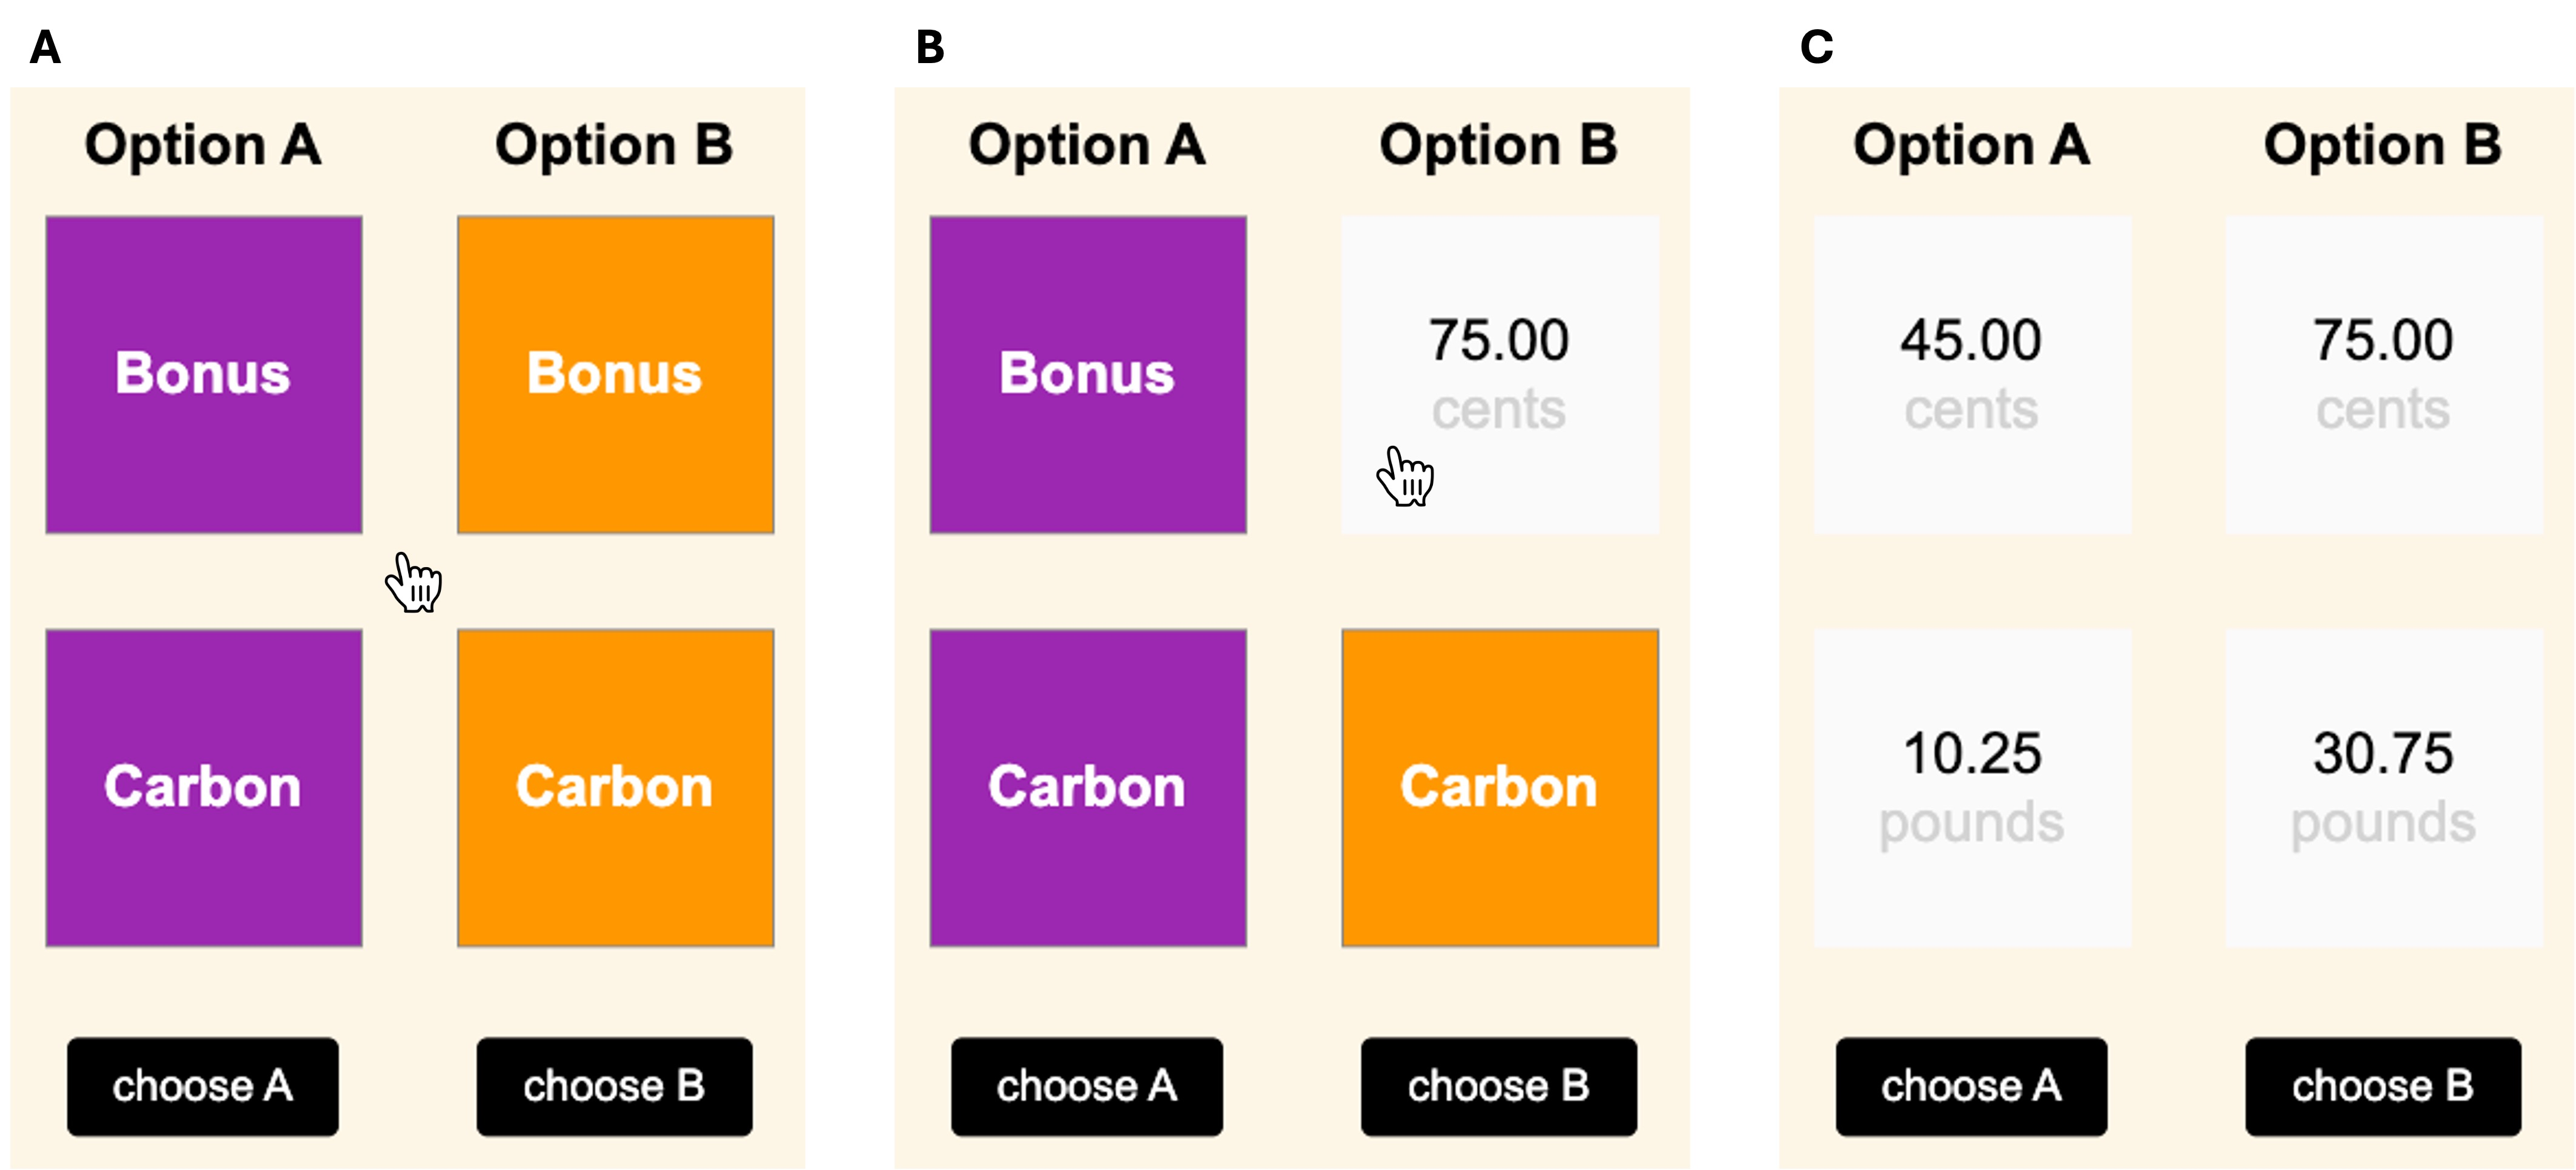
\includegraphics{../images/mouselabWEB_decisionScreen.jpg}

}

\caption{\label{fig-decisionScreen}An example trial of the new variant
of the CET. \textbf{(A)} Participants are presented with two options
which are associated with different bonus payment and carbon emission
consequences. \textbf{(B)} Participants inspect the exact consequences
regarding each attribute of each option by hovering their mouse over the
respective boxes. Moving the mouse outside of a box occludes the
information again. Note that whether the bonus or carbon attributes are
displayed in the top row is randomized across participants but held
constant within participants. \textbf{(C)} By visiting all boxes,
participants can acquire all available information in a trial (all boxes
opened simultaneously for demonstration purposes only). Note that
whether the option maximizing the bonus payment for participants is
presented in the left or right row is randomized within participants.}

\end{figure}%

In all analyses, the criterion (dependent variable) will be ΔDuration
(\texttt{deltaDuration}), which is calculated in each trial as:

\[
\Delta Duration = \frac{(t_{Carbon_{A}} + t_{Carbon_{B}}) - (t_{Bonus_{A}} + t_{Bonus_{B}})}{t_{Carbon_{A}} + t_{Carbon_{B}} + t_{Bonus_{A}} + t_{Bonus_{B}}}
\]

with \(t\) representing the summed up dwell time on \(Carbon/Bonus\)
boxes in Option \(A/B\). ΔDuration varies between -1 and 1 with:

\begin{itemize}
\tightlist
\item
  a value of -1 indicating that the entire dwell time was spent on
  gathering Bonus information
\item
  a value of 0 indicating that the dwell time was equally split between
  gathering Bonus and Carbon information
\item
  a value of 1 indication that the entire dwell time was spent on
  gathering Carbon information
\end{itemize}

\subsection{Political Affiliation}\label{political-affiliation}

We will assess political affiliation using the following question:

\emph{Generally speaking, do you think of yourself as a Democrat,
Republican or Independent?}

Participants will answer on the following 7-point Likert scale:

\emph{{[}1{]} Strong Republican, {[}2{]} Not strong Republican, {[}3{]}
Independent, close to Republican, {[}4{]} Independent, {[}5{]}
Independent, close to Democrat, {[}6{]} Not strong Democrat, {[}7{]}
Strong Democrat}

Additionally, if participants self-identify as {[}4{]} Independent, they
will be asked:

\emph{You said that you think of yourself as an Independent politically.
If you had to identify with one party of the two parties, which one
would you choose?}

Participants will answer on the following scale:

\emph{{[}1{]} Republican Party, {[}2{]} Democratic Party}

Based on these questions, we classify participants as either Republican
or Democrat as represented by the variable \texttt{polAff} that can take
on the following values:

\emph{{[}rep{]} Republican Party, {[}dem{]} Democratic Party}

\subsection{Extreme Weather Exposure}\label{extreme-weather-exposure}

For each participant, we will assess the number of extreme weather
episodes that occurred in the participants' county of residence in the
30 days prior to study completion. We then create a variable
\texttt{ewe} which equals to \emph{TRUE} if at least one extreme weather
episode occurred in the specified time interval, and \emph{FALSE}
otherwise.

\subsection{Subjective Attribution}\label{subjective-attribution}

We will assess the degree to which participants attribute extreme
weather events to climate change (see Ogunbode et al. 2019).
Participants will rate their agreement to the following three questions:

\begin{enumerate}
\def\labelenumi{\arabic{enumi}.}
\item
  \emph{Extreme weather events are caused in part by climate change.}
\item
  \emph{Extreme weather events are a sign that the impacts of climate
  change are happening now.}
\item
  \emph{Extreme weather events show us what we can expect from climate
  change in the future.}
\end{enumerate}

Participants will answer on the following 5-point Likert scale:

\emph{{[}1{]} Strongly disagree, {[}2{]} Somewhat disagree, {[}3{]}
Neither agree nor disagree, {[}4{]} Somewhat agree, {[}5{]} Strongly
agree}

Subjective attribution of EWE to climate change will be operationalised
as the mean agreement to these three statements. Note that Ogunbode et
al. (2019), who used the same questions, response options, and
aggregation, report a mean of 3.67 and a SD of 0.85 for this variable.

\section{SESOI}\label{sesoi}

As argued in the Registered Report, we hypothesize that
(H\textsubscript{1}) compared to Republicans, Democrats prioritize
searching for and attending to carbon over bonus information during
decision-making in the CET. That is, Democrats display higher ΔDuration
values compared to Republicans.

While H\textsubscript{1} describes the direction of the expected effect,
it does not specify the expected magnitude of the effect. This later
point is clarified by asking the question what would be the smallest
effect size that researchers would still consider theoretically
relevant, i.e., what is the smallest effect size of interest (SESOI)? We
argue for such a SESOI on theoretical grounds and based on previous
MouselabWEB research.

In mouselabWEB studies, it is standard practice to filter out any
information acquisition lasting less than 200 msec because such very
short (spurious) acquisitions are very unlikely to be consciously
processed (Willemsen and Johnson 2019). Therefore, we derive the SESOI
based on the consideration that for an effect to be meaningful, the
increase in ΔDuration from a Republican to a Democrat should be due to
an increase of the time spent gathering carbon (relative to bonus)
information of at least 200 msec. We need to translate these
considerations into the metric of ΔDuration.

Suppose that Republicans on average spend \(t_{Carbon}\) msec on
gathering carbon information and \(t_{Bonus}\) msec on gathering bonus
information in each trial, with a total time of gathering any
information \(t_{Total} = t_{Carbon} + t_{Bonus}\). Thus, for
Republicans, this results in:

\[
\Delta Duration_{Rep} = \frac{t_{Carbon} - t_{Bonus}}{t_{Total}}
\]

Suppose that Democrats have the same \(t_{Total}\) as Republicans, but
they spend 200 msec more on gathering carbon information and,
correspondingly, 200 msec less on gathering bonus information. Thus, for
Democrats, this results in:

\[
\Delta Duration_{Dem} = \frac{(t_{Carbon} + 200) - (t_{Bonus} - 200)}{t_{Total}} \\
                      = \frac{400 + t_{Carbon} - t_{Bonus}}{t_{Total}}
\]

Therefore, the difference in \(\Delta Duration\) for Democrats and
Republicans is:

\[
\begin{split}
\Delta Duration_{Dem} - \Delta Duration_{Rep} = \frac{400 + t_{Carbon} - t_{Bonus}}{t_{Total}} -  \frac{t_{Carbon} - t_{Bonus}}{t_{Total}} \\
  = \frac {(400 + t_{Carbon} - t_{Bonus}) - (t_{Carbon} - t_{Bonus})}{t_{Total}} \\
  = \frac {400}{t_{Total}}
\end{split}
\]

Thus, we define our SESOI as:

\[SESOI_{polAff} = \frac{400\ msec}{t_{Total}}\]

As this definition shows, the SESOI depends on our expectation regarding
\(t_{Total}\). We form these expectations based on previous research. In
our lab, we recently conducted another MouselabWEB study whose setup was
very similar to the one described in the Registered Report (Studler et
al., in preparation). In short, student participants completed a
behavioral task in which they searched for and attended to information
presented in a 2-by-2 decision matrix adapted from Reeck, Wall, and
Johnson (2017). The average time participants spent on acquiring
information in each trial (\(t_{Total}\)) was 3.3 seconds. In the
planned study we will assess a representative US sample. That is, the
average age of our sample will be higher than in a typical student
sample. As processing speed is known to decline with age (Salthouse
2000), we assume a slightly higher total information acquisition time in
our sample of \(t_{Total} = 3500\ msec\). Therefore, we define our SESOI
as:

\[
SESOI_{polAff} = \frac{400\ msec}{3500\ msec} = 0.1143
\]

To account for uncertainty in this estimation, we also provide
sample-size determination analysis results based on
\(t_{Total} = 4000\ msec\) and \(t_{Total} = 3000\ msec\). This results
in a high and low estimate of SESOI:

\[
\begin{split}
SESOI_{polAff_{high}} = \frac{400\ msec}{3000\ msec} = 0.1333 \\
SESOI_{polAff_{low}} = \frac{400\ msec}{4000\ msec} = 0.1000
\end{split}
\]

\section{Main Effect}\label{main-effect}

As argued in the Registered Report, we hypothesize:

\textbf{(H\textsubscript{1})} \emph{Compared to Republicans, Democrats
prioritize searching for and attending to carbon over bonus information
during decision-making in the CET. That is, Democrats display higher
ΔDuration values compared to Republicans.}

\begin{Shaded}
\begin{Highlighting}[]
\CommentTok{\# Create a data frame with predicted true effects}

\CommentTok{\# Smallest Effect Size Of Interest (SESOI)}
\NormalTok{SESOI }\OtherTok{\textless{}{-}} \FloatTok{0.4}\SpecialCharTok{/}\FloatTok{3.5}

\CommentTok{\# Betas}
\NormalTok{beta\_p }\OtherTok{\textless{}{-}}\NormalTok{ SESOI}

\CommentTok{\# Predicted "true" effects}
\NormalTok{polAff\_trueEffects }\OtherTok{\textless{}{-}} \FunctionTok{expand\_grid}\NormalTok{(}
  \AttributeTok{polAff =} \FunctionTok{factor}\NormalTok{(}\FunctionTok{c}\NormalTok{(}\StringTok{"rep"}\NormalTok{, }\StringTok{"dem"}\NormalTok{), }\AttributeTok{levels =} \FunctionTok{c}\NormalTok{(}\StringTok{"rep"}\NormalTok{, }\StringTok{"dem"}\NormalTok{))}
\NormalTok{) }\SpecialCharTok{\%\textgreater{}\%} 
  \FunctionTok{add\_contrast}\NormalTok{(}\StringTok{"polAff"}\NormalTok{, }\AttributeTok{contrast =} \StringTok{"anova"}\NormalTok{, }\AttributeTok{colnames =} \StringTok{"X\_p"}\NormalTok{) }\SpecialCharTok{\%\textgreater{}\%} 
  \FunctionTok{mutate}\NormalTok{(}
    \AttributeTok{trueDeltaDuration =}
      \DecValTok{0} \SpecialCharTok{+}         \CommentTok{\# intercept}
\NormalTok{      X\_p }\SpecialCharTok{*}\NormalTok{ beta\_p }\CommentTok{\# main effect polAff}
\NormalTok{  )}
\end{Highlighting}
\end{Shaded}

\subsection{Data Simulation Function}\label{data-simulation-function}

We first define a function that simulates data for the main effect of
political affiliation on ΔDuration: \texttt{FUN\_sim}. The function will
simulate data according to the following model, expressed in lme4-lingo:

\texttt{deltaDuration\ \textasciitilde{}\ polAff\ +\ (1\textbar{}subj)\ +\ (1\textbar{}trial)}

The function \texttt{FUN\_sim} takes, among others, the following
important arguments:

\begin{itemize}
\item
  \texttt{n\_subj}: \textbf{Number of subjects}. Chaning this parameter
  allows us to assess statistical power for different sample sizes.
\item
  \texttt{beta\_0}: \textbf{Fixed intercept (grand mean)}. We assume
  that the average participant (irrespective of political affiliation or
  any other predictor variable) spends about the same time on searching
  for and attending to carbon as to bonus information in the CET.
  Therefore, we set \texttt{beta\_0} to zero. The effects of predictor
  variables will be modeled as deviations from this grand mean.
\item
  \texttt{beta\_p}: \textbf{Fixed effect of political affiliation}. This
  value represents the average difference in ΔDuration between Democrats
  and Republicans (Democrats - Republicans). As discussed above, we set
  this value to 0.1143 by default, and we assess the effect of changing
  this variable on statistical power.
\item
  \texttt{subj\_0}: \textbf{By-subject random intercept SD}. We simulate
  that a participants' deviations from the grand mean for ΔDuration
  follows a normal distribution with a mean of 0 and a standard
  deviation of \texttt{subj\_0} = 0.29. We base our default value on a
  study by Reeck, Wall, and Johnson (2017). They investigated whether
  variability in information search behavior is driven predominantly by
  differences in the features of a choice (i.e., in our case: the
  relative differences between carbon and bonus outcomes in options A
  and B) or by individual differences. To this end, they predicted
  information acquisition using a intercept-only model that included
  random intercepts for subjects and items. They estimated the random
  intercept of subjects to be 0.29.
\item
  \texttt{trial\_0}: \textbf{By-trial random intercept SD}. We simulate
  that a items' deviations from the grand mean for ΔDuration follows a
  normal distribution with a mean of 0 and a standard deviation of
  \texttt{trial\_0} = 0.04. Again, we base our default value on the
  study by Reeck, Wall, and Johnson (2017), who estimated a random
  intercept for trials of 0.04.
\item
  \texttt{sigma}: \textbf{Trial-level noise (error) SD}. We model the
  error SD to be of the same size as the sum of the random intercept SDs
  = 0.29 + 0.04 = 0.33. We also report simulation results for an error
  SD that is twice the size of the random intercept SDs, i.e., 0.66.
\end{itemize}

The function \texttt{FUN\_sim} is defined below:

\begin{Shaded}
\begin{Highlighting}[]
\CommentTok{\# define data simulation function}
\NormalTok{FUN\_sim }\OtherTok{\textless{}{-}} \ControlFlowTok{function}\NormalTok{(}
  \AttributeTok{n\_subj       =}        \DecValTok{1000}\NormalTok{, }\CommentTok{\# number of subjects}
  \AttributeTok{n\_subj\_prop  =}   \FunctionTok{c}\NormalTok{(.}\DecValTok{5}\NormalTok{, .}\DecValTok{5}\NormalTok{), }\CommentTok{\# proportion of republican and democrat subjects}
  \AttributeTok{n\_trial      =}          \DecValTok{25}\NormalTok{, }\CommentTok{\# number of trials}
  \AttributeTok{beta\_0       =}           \DecValTok{0}\NormalTok{, }\CommentTok{\# intercept (grand mean) for deltaDuration}
  \AttributeTok{beta\_p       =}     \FloatTok{0.4}\SpecialCharTok{/}\FloatTok{3.5}\NormalTok{, }\CommentTok{\# effect of political affiliation on deltaDuration}
  \AttributeTok{subj\_0       =}\NormalTok{         .}\DecValTok{29}\NormalTok{, }\CommentTok{\# by{-}subject random intercept sd for dt carbon}
  \AttributeTok{trial\_0      =}\NormalTok{         .}\DecValTok{04}\NormalTok{, }\CommentTok{\# by{-}trial random intercept sd}
  \AttributeTok{sigma        =} \DecValTok{1}\SpecialCharTok{*}\NormalTok{(.}\DecValTok{29}\FloatTok{+.04}\NormalTok{), }\CommentTok{\# residual (error) sd}
  
  \AttributeTok{truncNums    =}        \ConstantTok{TRUE}\NormalTok{, }\CommentTok{\# should impossible deltaDuration values be truncuated?}
  \AttributeTok{setSeed      =}        \ConstantTok{NULL}  \CommentTok{\# seed number to achieve reproducible results. Set to NULL for simulations!}
\NormalTok{) \{}
  
  \CommentTok{\# set seed to achieve reproducible results for demonstration purposes}
  \FunctionTok{set.seed}\NormalTok{(setSeed)}
  
  \CommentTok{\# simulate data for dwell time on carbon information}
\NormalTok{  dataSim }\OtherTok{\textless{}{-}} 
    \CommentTok{\# add random factor subject}
    \FunctionTok{add\_random}\NormalTok{(}\AttributeTok{subj =}\NormalTok{ n\_subj) }\SpecialCharTok{\%\textgreater{}\%} 
    \CommentTok{\# add random factor trial}
    \FunctionTok{add\_random}\NormalTok{(}\AttributeTok{trial =}\NormalTok{ n\_trial) }\SpecialCharTok{\%\textgreater{}\%} 
    \CommentTok{\# add between{-}subject factor political affiliation (with anova contrast)}
    \FunctionTok{add\_between}\NormalTok{(}\StringTok{"subj"}\NormalTok{, }\AttributeTok{polAff =} \FunctionTok{c}\NormalTok{(}\StringTok{"rep"}\NormalTok{, }\StringTok{"dem"}\NormalTok{), }\AttributeTok{.prob =}\NormalTok{ n\_subj\_prop}\SpecialCharTok{*}\NormalTok{n\_subj, }\AttributeTok{.shuffle =} \ConstantTok{FALSE}\NormalTok{) }\SpecialCharTok{\%\textgreater{}\%} 
    \FunctionTok{add\_contrast}\NormalTok{(}\StringTok{"polAff"}\NormalTok{, }\AttributeTok{colnames =} \StringTok{"X\_p"}\NormalTok{, }\AttributeTok{contrast =} \StringTok{"anova"}\NormalTok{) }\SpecialCharTok{\%\textgreater{}\%} 
    \CommentTok{\# add by{-}subject random intercept}
    \FunctionTok{add\_ranef}\NormalTok{(}\StringTok{"subj"}\NormalTok{, }\AttributeTok{S\_0 =}\NormalTok{ subj\_0) }\SpecialCharTok{\%\textgreater{}\%} 
    \CommentTok{\# add by{-}trial random intercept}
    \FunctionTok{add\_ranef}\NormalTok{(}\StringTok{"trial"}\NormalTok{, }\AttributeTok{T\_0 =}\NormalTok{ trial\_0) }\SpecialCharTok{\%\textgreater{}\%} 
    \CommentTok{\# add error term}
    \FunctionTok{add\_ranef}\NormalTok{(}\AttributeTok{e\_st =}\NormalTok{ sigma) }\SpecialCharTok{\%\textgreater{}\%} 
    \CommentTok{\# add response values}
    \FunctionTok{mutate}\NormalTok{(}
      \CommentTok{\# add together fixed and random effects for each effect}
      \AttributeTok{B\_0 =}\NormalTok{ beta\_0 }\SpecialCharTok{+}\NormalTok{ S\_0 }\SpecialCharTok{+}\NormalTok{ T\_0,}
      \AttributeTok{B\_p =}\NormalTok{ beta\_p,}
      \CommentTok{\# calculate dv by adding each effect term multiplied by the relevant}
      \CommentTok{\# effect{-}coded factors and adding the error term}
      \AttributeTok{deltaDuration =}\NormalTok{ B\_0 }\SpecialCharTok{+}\NormalTok{ (B\_p }\SpecialCharTok{*}\NormalTok{ X\_p) }\SpecialCharTok{+}\NormalTok{ e\_st}
\NormalTok{    )}
  
  \CommentTok{\# unset seed}
  \FunctionTok{set.seed}\NormalTok{(}\ConstantTok{NULL}\NormalTok{)}
  
  \CommentTok{\# truncuate impossible deltaDurations}
  \ControlFlowTok{if}\NormalTok{(truncNums) \{}
\NormalTok{    dataSim }\OtherTok{\textless{}{-}}\NormalTok{ dataSim }\SpecialCharTok{\%\textgreater{}\%} 
      \FunctionTok{mutate}\NormalTok{(}\AttributeTok{deltaDuration =} \FunctionTok{if\_else}\NormalTok{(deltaDuration }\SpecialCharTok{\textless{}} \SpecialCharTok{{-}}\DecValTok{1}\NormalTok{, }\SpecialCharTok{{-}}\DecValTok{1}\NormalTok{,}
        \FunctionTok{if\_else}\NormalTok{(deltaDuration }\SpecialCharTok{\textgreater{}} \DecValTok{1}\NormalTok{, }\DecValTok{1}\NormalTok{, deltaDuration)))}
\NormalTok{  \}}
  
  \CommentTok{\# run a linear mixed effects model and check summary}
\NormalTok{  mod }\OtherTok{\textless{}{-}} \FunctionTok{lmer}\NormalTok{(}
\NormalTok{    deltaDuration }\SpecialCharTok{\textasciitilde{}}\NormalTok{ polAff }\SpecialCharTok{+}\NormalTok{ (}\DecValTok{1} \SpecialCharTok{|}\NormalTok{ subj) }\SpecialCharTok{+}\NormalTok{ (}\DecValTok{1} \SpecialCharTok{|}\NormalTok{ trial),}
    \AttributeTok{data =}\NormalTok{ dataSim,}
\NormalTok{  )}
\NormalTok{  mod.sum }\OtherTok{\textless{}{-}} \FunctionTok{summary}\NormalTok{(mod)}
  
  \CommentTok{\# get results in tidy format}
\NormalTok{  mod.broom }\OtherTok{\textless{}{-}}\NormalTok{ broom.mixed}\SpecialCharTok{::}\FunctionTok{tidy}\NormalTok{(mod)}
  
  \FunctionTok{return}\NormalTok{(}\FunctionTok{list}\NormalTok{(}
    \AttributeTok{dataSim =}\NormalTok{ dataSim,}
    \AttributeTok{modelLmer =}\NormalTok{ mod,}
    \AttributeTok{modelResults =}\NormalTok{ mod.broom}
\NormalTok{  ))}
  
\NormalTok{\}}
\end{Highlighting}
\end{Shaded}

We call the function once and extract the results of this single
simulation:

\begin{Shaded}
\begin{Highlighting}[]
\CommentTok{\# Call function}
\NormalTok{out }\OtherTok{\textless{}{-}} \FunctionTok{FUN\_sim}\NormalTok{(}
  \AttributeTok{n\_subj       =}        \DecValTok{1000}\NormalTok{, }\CommentTok{\# number of subjects}
  \AttributeTok{n\_subj\_prop  =}   \FunctionTok{c}\NormalTok{(.}\DecValTok{5}\NormalTok{, .}\DecValTok{5}\NormalTok{), }\CommentTok{\# proportion of republican and democrat subjects}
  \AttributeTok{n\_trial      =}          \DecValTok{25}\NormalTok{, }\CommentTok{\# number of trials}
  \AttributeTok{beta\_0       =}           \DecValTok{0}\NormalTok{, }\CommentTok{\# intercept (grand mean) for deltaDuration}
  \AttributeTok{beta\_p       =}     \FloatTok{0.4}\SpecialCharTok{/}\FloatTok{3.5}\NormalTok{, }\CommentTok{\# effect of political affiliation on deltaDuration}
  \AttributeTok{subj\_0       =}\NormalTok{         .}\DecValTok{29}\NormalTok{, }\CommentTok{\# by{-}subject random intercept sd for dt carbon}
  \AttributeTok{trial\_0      =}\NormalTok{         .}\DecValTok{04}\NormalTok{, }\CommentTok{\# by{-}trial random intercept sd}
  \AttributeTok{sigma        =} \DecValTok{1}\SpecialCharTok{*}\NormalTok{(.}\DecValTok{29}\FloatTok{+.04}\NormalTok{), }\CommentTok{\# residual (error) sd}
  
  \AttributeTok{truncNums    =}        \ConstantTok{TRUE}\NormalTok{, }\CommentTok{\# should impossible deltaDuration values be truncuated?}
  \AttributeTok{setSeed      =}        \DecValTok{1234}  \CommentTok{\# seed number to achieve reproducible results. Set to NULL for simulations!}
\NormalTok{)}

\CommentTok{\# Get results table}
\NormalTok{resultsTable }\OtherTok{\textless{}{-}}\NormalTok{ out}\SpecialCharTok{$}\NormalTok{modelResults }\SpecialCharTok{\%\textgreater{}\%} 
  \FunctionTok{select}\NormalTok{(}\SpecialCharTok{{-}}\FunctionTok{c}\NormalTok{(std.error, statistic, df)) }\SpecialCharTok{\%\textgreater{}\%} 
  \FunctionTok{mutate}\NormalTok{(}\FunctionTok{across}\NormalTok{(}\FunctionTok{where}\NormalTok{(is\_double), }\SpecialCharTok{\textasciitilde{}} \FunctionTok{round}\NormalTok{(.x, }\DecValTok{4}\NormalTok{))) }\SpecialCharTok{\%\textgreater{}\%} 
\NormalTok{  knitr}\SpecialCharTok{::}\FunctionTok{kable}\NormalTok{()}
\NormalTok{formulaUsedForFit }\OtherTok{\textless{}{-}} \FunctionTok{paste}\NormalTok{(}\FunctionTok{as.character}\NormalTok{(}\FunctionTok{formula}\NormalTok{(out}\SpecialCharTok{$}\NormalTok{modelLmer))[}\FunctionTok{c}\NormalTok{(}\DecValTok{2}\NormalTok{,}\DecValTok{1}\NormalTok{,}\DecValTok{3}\NormalTok{)], }\AttributeTok{collapse =} \StringTok{" "}\NormalTok{)}

\CommentTok{\# Create plot}
\NormalTok{p.demo.mainEffect }\OtherTok{\textless{}{-}}\NormalTok{  out}\SpecialCharTok{$}\NormalTok{dataSim }\SpecialCharTok{\%\textgreater{}\%} 
  \FunctionTok{ggplot}\NormalTok{(}\FunctionTok{aes}\NormalTok{(}\AttributeTok{x =}\NormalTok{ polAff, }\AttributeTok{y =}\NormalTok{ deltaDuration, }\AttributeTok{color =}\NormalTok{ polAff)) }\SpecialCharTok{+}
  \FunctionTok{geom\_hline}\NormalTok{(}\AttributeTok{yintercept =} \DecValTok{0}\NormalTok{) }\SpecialCharTok{+}
  \FunctionTok{geom\_violin}\NormalTok{(}\AttributeTok{alpha =} \FloatTok{0.3}\NormalTok{) }\SpecialCharTok{+}
  \FunctionTok{geom\_point}\NormalTok{(}
    \AttributeTok{data =}\NormalTok{ polAff\_trueEffects,}
    \AttributeTok{mapping =} \FunctionTok{aes}\NormalTok{(}\AttributeTok{x =}\NormalTok{ polAff, }\AttributeTok{y =}\NormalTok{ trueDeltaDuration),}
    \AttributeTok{shape =} \StringTok{"circle open"}\NormalTok{,}
    \AttributeTok{size =} \FloatTok{3.5}\NormalTok{,}
    \AttributeTok{stroke =} \DecValTok{2}\NormalTok{,}
    \AttributeTok{color =} \StringTok{"black"}
\NormalTok{  ) }\SpecialCharTok{+}
  \FunctionTok{stat\_summary}\NormalTok{(}
    \AttributeTok{fun =}\NormalTok{ mean,}
    \AttributeTok{fun.min =}\NormalTok{ \textbackslash{}(x)\{}\FunctionTok{mean}\NormalTok{(x) }\SpecialCharTok{{-}} \FunctionTok{sd}\NormalTok{(x)\},}
    \AttributeTok{fun.max =}\NormalTok{ \textbackslash{}(x)\{}\FunctionTok{mean}\NormalTok{(x) }\SpecialCharTok{+} \FunctionTok{sd}\NormalTok{(x)\},}
    \AttributeTok{position =} \FunctionTok{position\_dodge}\NormalTok{(}\AttributeTok{width =}\NormalTok{ .}\DecValTok{9}\NormalTok{)}
\NormalTok{  ) }\SpecialCharTok{+}
\NormalTok{  ggrepel}\SpecialCharTok{::}\FunctionTok{geom\_label\_repel}\NormalTok{(}
    \AttributeTok{data =}\NormalTok{ polAff\_trueEffects,}
    \AttributeTok{mapping =} \FunctionTok{aes}\NormalTok{(}\AttributeTok{x =}\NormalTok{ polAff, }\AttributeTok{y =}\NormalTok{ trueDeltaDuration, }\AttributeTok{label =} \FunctionTok{round}\NormalTok{(trueDeltaDuration, }\DecValTok{4}\NormalTok{)),}
    \AttributeTok{color =} \StringTok{"black"}\NormalTok{,}
    \AttributeTok{box.padding =} \DecValTok{1}
\NormalTok{  ) }\SpecialCharTok{+}
  \FunctionTok{scale\_color\_manual}\NormalTok{(}\AttributeTok{values =} \FunctionTok{c}\NormalTok{(}\StringTok{"red"}\NormalTok{, }\StringTok{"dodgerblue"}\NormalTok{)) }\SpecialCharTok{+}
  \FunctionTok{scale\_y\_continuous}\NormalTok{(}\AttributeTok{breaks =} \FunctionTok{seq}\NormalTok{(}\SpecialCharTok{{-}}\DecValTok{1}\NormalTok{, }\DecValTok{1}\NormalTok{, .}\DecValTok{2}\NormalTok{)) }\SpecialCharTok{+}
  \FunctionTok{labs}\NormalTok{(}\AttributeTok{title =} \StringTok{"Demo Output of One Simulation for Main Effect"}\NormalTok{) }\SpecialCharTok{+}
  \FunctionTok{theme\_bw}\NormalTok{() }\SpecialCharTok{+}
  \FunctionTok{theme}\NormalTok{(}\AttributeTok{legend.position =} \StringTok{"none"}\NormalTok{)}
\end{Highlighting}
\end{Shaded}

Figure~\ref{fig-demoFUNSim} visualizes the results of this single
simulation and Table~\ref{tbl-demoFUNSim} summarises the statistical
results of fitting the actual model used in data generation to the
simulated data.

\begin{figure}

\centering{

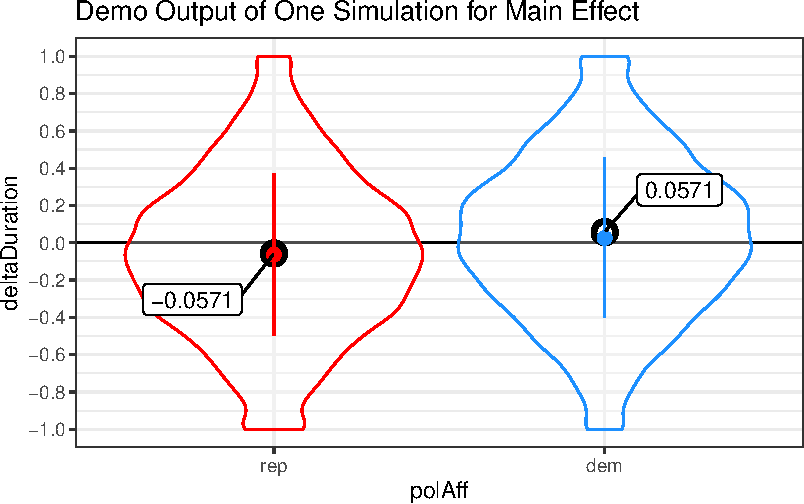
\includegraphics{powerSimulations_files/figure-pdf/fig-demoFUNSim-1.pdf}

}

\caption{\label{fig-demoFUNSim}Visual representation of results of one
simulation created using \texttt{FUN\_sim}. Violin plots display the
full distribution of the data. Points and surrounding lines indicate the
mean ± 1 SD. The black horizontal line displays the true sample mean and
the black open circles indicate the true means for each cell.}

\end{figure}%

\phantomsection\label{tbl-demoFUNSim}
\begin{longtable}[]{@{}lllrr@{}}

\caption{\label{tbl-demoFUNSim}Statistical results of one simulation
created using \texttt{FUN\_sim}. Data was fit using deltaDuration
\textasciitilde{} polAff + (1 \textbar{} subj) + (1 \textbar{} trial).}

\tabularnewline

\toprule\noalign{}
effect & group & term & estimate & p.value \\
\midrule\noalign{}
\endhead
\bottomrule\noalign{}
\endlastfoot
fixed & NA & (Intercept) & -0.0188 & 0.1105 \\
fixed & NA & polAff.dem-rep & 0.0896 & 0.0000 \\
ran\_pars & subj & sd\_\_(Intercept) & 0.2841 & NA \\
ran\_pars & trial & sd\_\_(Intercept) & 0.0363 & NA \\
ran\_pars & Residual & sd\_\_Observation & 0.3223 & NA \\

\end{longtable}

\subsection{Power Simulation}\label{power-simulation}

We now simulate multiple random samples drawn from the same synthetic
population with a known true effect of political affiliation. For each
random sample, we fit our statistical model to the data. The statistical
power to detect a true effect of political affiliation is calculated as
the proportion of significant effects out of the total number of
simulations. We aim for a statistical power of 95\%.

In the following code, the simulations are calculated. We do not
recommend executing this code junk as it takes several hours to run.

\begin{Shaded}
\begin{Highlighting}[]
\NormalTok{FUN\_sim\_pwr }\OtherTok{\textless{}{-}} \ControlFlowTok{function}\NormalTok{(sim, ...)\{}
\NormalTok{  out }\OtherTok{\textless{}{-}} \FunctionTok{FUN\_sim}\NormalTok{(...)}
\NormalTok{  modelResults }\OtherTok{\textless{}{-}}\NormalTok{ out}\SpecialCharTok{$}\NormalTok{modelResults }\SpecialCharTok{\%\textgreater{}\%} 
    \FunctionTok{mutate}\NormalTok{(}\AttributeTok{sim =}\NormalTok{ sim) }\SpecialCharTok{\%\textgreater{}\%} 
    \FunctionTok{relocate}\NormalTok{(sim)}
  \FunctionTok{return}\NormalTok{(modelResults)}
\NormalTok{\}}

\CommentTok{\# How many simulations should be run?}
\NormalTok{n\_sims }\OtherTok{\textless{}{-}} \DecValTok{1000}

\CommentTok{\# What are the breaks for number of subjects we would like to calculate power for?}
\NormalTok{breaks\_subj }\OtherTok{\textless{}{-}} \FunctionTok{seq}\NormalTok{(}\DecValTok{200}\NormalTok{, }\DecValTok{1000}\NormalTok{, }\DecValTok{200}\NormalTok{)}

\CommentTok{\# What are the breaks for SESOI?}
\NormalTok{breaks\_sesoi }\OtherTok{\textless{}{-}} \FunctionTok{c}\NormalTok{(}\FloatTok{0.4}\SpecialCharTok{/}\DecValTok{3}\NormalTok{, }\FloatTok{0.4}\SpecialCharTok{/}\FloatTok{3.5}\NormalTok{, }\FloatTok{0.4}\SpecialCharTok{/}\DecValTok{4}\NormalTok{)}

\CommentTok{\# What are the breaks for different errer SDs?}
\NormalTok{breaks\_sigma }\OtherTok{\textless{}{-}} \FunctionTok{c}\NormalTok{(}\DecValTok{1}\SpecialCharTok{:}\DecValTok{2}\NormalTok{)}\SpecialCharTok{*}\NormalTok{(.}\DecValTok{29}\FloatTok{+.04}\NormalTok{)}

\NormalTok{res\_mainEffect }\OtherTok{\textless{}{-}} \FunctionTok{tibble}\NormalTok{()}
\ControlFlowTok{for}\NormalTok{ (s }\ControlFlowTok{in} \FunctionTok{seq\_along}\NormalTok{(breaks\_sigma)) \{}
  
\NormalTok{  res\_sesoi }\OtherTok{\textless{}{-}} \FunctionTok{tibble}\NormalTok{()}
  \ControlFlowTok{for}\NormalTok{ (sesoi }\ControlFlowTok{in} \FunctionTok{seq\_along}\NormalTok{(breaks\_sesoi)) \{}
    
\NormalTok{    res\_nSubj }\OtherTok{\textless{}{-}} \FunctionTok{tibble}\NormalTok{()}
    \ControlFlowTok{for}\NormalTok{ (nSubj }\ControlFlowTok{in} \FunctionTok{seq\_along}\NormalTok{(breaks\_subj)) \{}
      
      \CommentTok{\# Give feedback regarding which model is simulated}
      \FunctionTok{cat}\NormalTok{(}\FunctionTok{paste0}\NormalTok{(}
        \StringTok{"Simulation:}\SpecialCharTok{\textbackslash{}n}\StringTok{"}\NormalTok{,}
        \StringTok{"  sigma = "}\NormalTok{, }\FunctionTok{round}\NormalTok{(breaks\_sigma[s], }\DecValTok{4}\NormalTok{), }\StringTok{"}\SpecialCharTok{\textbackslash{}n}\StringTok{"}\NormalTok{,}
        \StringTok{"  sesoi = "}\NormalTok{, }\FunctionTok{round}\NormalTok{(breaks\_sesoi[sesoi], }\DecValTok{4}\NormalTok{), }\StringTok{"}\SpecialCharTok{\textbackslash{}n}\StringTok{"}\NormalTok{,}
        \StringTok{"  nSubject = "}\NormalTok{, breaks\_subj[nSubj], }\StringTok{"}\SpecialCharTok{\textbackslash{}n}\StringTok{"}
\NormalTok{      ))}
      
      \CommentTok{\# Start timer}
      \FunctionTok{cat}\NormalTok{(}\FunctionTok{paste0}\NormalTok{(}\StringTok{"Start date time: "}\NormalTok{, lubridate}\SpecialCharTok{::}\FunctionTok{now}\NormalTok{(), }\StringTok{"}\SpecialCharTok{\textbackslash{}n}\StringTok{"}\NormalTok{))}
      \FunctionTok{tic}\NormalTok{()}
      
      \CommentTok{\# Loop over simulations}
\NormalTok{      pwr }\OtherTok{\textless{}{-}} \FunctionTok{map\_df}\NormalTok{(}
        \DecValTok{1}\SpecialCharTok{:}\NormalTok{n\_sims, }
\NormalTok{        FUN\_sim\_pwr,}
        \AttributeTok{n\_subj =}\NormalTok{ breaks\_subj[nSubj],}
        \AttributeTok{beta\_p =}\NormalTok{ breaks\_sesoi[sesoi],}
        \AttributeTok{sigma =}\NormalTok{ breaks\_sigma[s]}
\NormalTok{      )}
      
      \CommentTok{\# Stop timer and calculate elapsed time}
\NormalTok{      elapsed\_time }\OtherTok{\textless{}{-}} \FunctionTok{toc}\NormalTok{(}\AttributeTok{quiet =} \ConstantTok{TRUE}\NormalTok{)}
\NormalTok{      elapsed\_seconds }\OtherTok{\textless{}{-}}\NormalTok{ elapsed\_time}\SpecialCharTok{$}\NormalTok{toc }\SpecialCharTok{{-}}\NormalTok{ elapsed\_time}\SpecialCharTok{$}\NormalTok{tic}
\NormalTok{      elapsed\_minutes }\OtherTok{\textless{}{-}}\NormalTok{ elapsed\_seconds }\SpecialCharTok{/} \DecValTok{60}
      \FunctionTok{cat}\NormalTok{(}\FunctionTok{paste0}\NormalTok{(}\StringTok{"End date time: "}\NormalTok{, lubridate}\SpecialCharTok{::}\FunctionTok{now}\NormalTok{(), }\StringTok{"}\SpecialCharTok{\textbackslash{}n}\StringTok{"}\NormalTok{))}
      \FunctionTok{cat}\NormalTok{(}\StringTok{"Elapsed time: "}\NormalTok{, elapsed\_minutes, }\StringTok{" minutes}\SpecialCharTok{\textbackslash{}n\textbackslash{}n}\StringTok{"}\NormalTok{)}
      
      \CommentTok{\# Add number of subjects to pwr}
\NormalTok{      pwr }\OtherTok{\textless{}{-}}\NormalTok{ pwr }\SpecialCharTok{\%\textgreater{}\%} 
        \FunctionTok{mutate}\NormalTok{(}
          \AttributeTok{nSubjects =}\NormalTok{ breaks\_subj[nSubj],}
          \AttributeTok{sesoi =}\NormalTok{ breaks\_sesoi[sesoi],}
          \AttributeTok{sigma =}\NormalTok{ breaks\_sigma[s]}
\NormalTok{        )}
      
      \CommentTok{\# Add results to the results table}
\NormalTok{      res\_nSubj }\OtherTok{\textless{}{-}}\NormalTok{ res\_nSubj }\SpecialCharTok{\%\textgreater{}\%}
        \FunctionTok{rbind}\NormalTok{(pwr)}
\NormalTok{    \}}
    
    \CommentTok{\# Add results to the results table}
\NormalTok{    res\_sesoi }\OtherTok{\textless{}{-}}\NormalTok{ res\_sesoi }\SpecialCharTok{\%\textgreater{}\%} 
      \FunctionTok{rbind}\NormalTok{(res\_nSubj)}
\NormalTok{  \}}
  
  \CommentTok{\# Add results to the results table}
\NormalTok{  res\_mainEffect }\OtherTok{\textless{}{-}}\NormalTok{ res\_mainEffect }\SpecialCharTok{\%\textgreater{}\%} 
    \FunctionTok{rbind}\NormalTok{(res\_sesoi)}
  
\NormalTok{\}}

\NormalTok{res\_mainEffect.summary }\OtherTok{\textless{}{-}}\NormalTok{ res\_mainEffect }\SpecialCharTok{\%\textgreater{}\%} 
  \FunctionTok{filter}\NormalTok{(term }\SpecialCharTok{==} \StringTok{"polAff.dem{-}rep"}\NormalTok{) }\SpecialCharTok{\%\textgreater{}\%} 
  \FunctionTok{group\_by}\NormalTok{(sigma, sesoi, nSubjects) }\SpecialCharTok{\%\textgreater{}\%} 
  \FunctionTok{summarise}\NormalTok{(}
    \AttributeTok{power =} \FunctionTok{mean}\NormalTok{(p.value }\SpecialCharTok{\textless{}} \FloatTok{0.05}\NormalTok{),}
    \AttributeTok{ci.lower =} \FunctionTok{binom.confint}\NormalTok{(power}\SpecialCharTok{*}\NormalTok{n\_sims, n\_sims, }\AttributeTok{methods =} \StringTok{"exact"}\NormalTok{)}\SpecialCharTok{$}\NormalTok{lower,}
    \AttributeTok{ci.upper =} \FunctionTok{binom.confint}\NormalTok{(power}\SpecialCharTok{*}\NormalTok{n\_sims, n\_sims, }\AttributeTok{methods =} \StringTok{"exact"}\NormalTok{)}\SpecialCharTok{$}\NormalTok{upper,}
    \AttributeTok{.groups =} \StringTok{\textquotesingle{}drop\textquotesingle{}}
\NormalTok{  ) }\SpecialCharTok{\%\textgreater{}\%} 
  \FunctionTok{mutate}\NormalTok{(}
    \AttributeTok{sigma\_fact =} \FunctionTok{factor}\NormalTok{(}\FunctionTok{format}\NormalTok{(}\FunctionTok{round}\NormalTok{(sigma, }\DecValTok{4}\NormalTok{), }\AttributeTok{nsmall =} \DecValTok{4}\NormalTok{)),}
    \AttributeTok{sigma\_level =} \FunctionTok{match}\NormalTok{(sigma\_fact, }\FunctionTok{levels}\NormalTok{(sigma\_fact)),}
    \AttributeTok{sesoi\_fact =} \FunctionTok{factor}\NormalTok{(}\FunctionTok{format}\NormalTok{(}\FunctionTok{round}\NormalTok{(sesoi, }\DecValTok{4}\NormalTok{), }\AttributeTok{nsmall =} \DecValTok{4}\NormalTok{)),}
    \AttributeTok{sesoi\_level =} \FunctionTok{match}\NormalTok{(sesoi\_fact, }\FunctionTok{levels}\NormalTok{(sesoi\_fact))}
\NormalTok{  )}

\CommentTok{\# Save results in a list object}
\NormalTok{time }\OtherTok{\textless{}{-}} \FunctionTok{format}\NormalTok{(}\FunctionTok{Sys.time}\NormalTok{(), }\StringTok{"\%Y\%m\%d\_\%H\%M"}\NormalTok{)}
\NormalTok{fileName }\OtherTok{\textless{}{-}} \FunctionTok{paste0}\NormalTok{(}\StringTok{"res\_mainEffect"}\NormalTok{, }\StringTok{"\_"}\NormalTok{, time, }\StringTok{".RDS"}\NormalTok{)}
\FunctionTok{saveRDS}\NormalTok{(}
  \FunctionTok{list}\NormalTok{(}
    \AttributeTok{res\_mainEffect =}\NormalTok{ res\_mainEffect,}
    \AttributeTok{res\_mainEffect.summary =}\NormalTok{ res\_mainEffect.summary}
\NormalTok{  ),}
  \AttributeTok{file =} \FunctionTok{file.path}\NormalTok{(}\StringTok{"../powerSimulationsOutput"}\NormalTok{, fileName)}
\NormalTok{)}
\end{Highlighting}
\end{Shaded}

We retrieve pre-run results:

\begin{Shaded}
\begin{Highlighting}[]
\CommentTok{\# Load power simulation data}
\NormalTok{resList\_mainEffect }\OtherTok{\textless{}{-}} \FunctionTok{readRDS}\NormalTok{(}\FunctionTok{file.path}\NormalTok{(}\StringTok{"../powerSimulationsOutput"}\NormalTok{, }\StringTok{"res\_mainEffect\_20240813\_2141.RDS"}\NormalTok{))}
\NormalTok{resList\_mainEffect.summary }\OtherTok{\textless{}{-}}\NormalTok{ resList\_mainEffect}\SpecialCharTok{$}\NormalTok{res\_mainEffect.summary}

\CommentTok{\# Extract power values for some specific effect sizes at N = 1000}
\NormalTok{chosenN }\OtherTok{\textless{}{-}} \DecValTok{600}
\NormalTok{chosenSigma }\OtherTok{\textless{}{-}} \FunctionTok{c}\NormalTok{(}\StringTok{"0.3300"}\NormalTok{, }\StringTok{"0.6600"}\NormalTok{)}
\NormalTok{chosenSESOI }\OtherTok{\textless{}{-}} \FunctionTok{c}\NormalTok{(}\StringTok{"0.1000"}\NormalTok{, }\StringTok{"0.1143"}\NormalTok{)}
\NormalTok{powerValues }\OtherTok{\textless{}{-}}\NormalTok{ resList\_mainEffect.summary }\SpecialCharTok{\%\textgreater{}\%} 
  \FunctionTok{filter}\NormalTok{(sigma\_fact }\SpecialCharTok{\%in\%}\NormalTok{ chosenSigma) }\SpecialCharTok{\%\textgreater{}\%} 
  \FunctionTok{filter}\NormalTok{(sesoi\_fact }\SpecialCharTok{\%in\%}\NormalTok{ chosenSESOI) }\SpecialCharTok{\%\textgreater{}\%} 
  \FunctionTok{filter}\NormalTok{(nSubjects }\SpecialCharTok{\%in\%}\NormalTok{ chosenN) }\SpecialCharTok{\%\textgreater{}\%} 
  \FunctionTok{mutate}\NormalTok{(}\AttributeTok{power\_str =} \FunctionTok{paste0}\NormalTok{(}\FunctionTok{round}\NormalTok{(ci.lower}\SpecialCharTok{*}\DecValTok{100}\NormalTok{, }\DecValTok{2}\NormalTok{), }\StringTok{"\%"}\NormalTok{)) }\SpecialCharTok{\%\textgreater{}\%} 
  \FunctionTok{pull}\NormalTok{(power\_str)}

\CommentTok{\# Extract number of simulations}
\NormalTok{label\_nSimulations }\OtherTok{\textless{}{-}}\NormalTok{ resList\_mainEffect}\SpecialCharTok{$}\NormalTok{res\_mainEffect}\SpecialCharTok{$}\NormalTok{sim }\SpecialCharTok{\%\textgreater{}\%} \FunctionTok{n\_distinct}\NormalTok{()}
\end{Highlighting}
\end{Shaded}

Figure~\ref{fig-checkSims-mainEffect} displays the distribution of
estimated fixed effects across all simulations. The figure shows that
the estimated fixed effects are close to the true ones provided as input
in the data simulation function, validating that simulations worked as
expected.

\begin{figure}

\centering{

\centering{

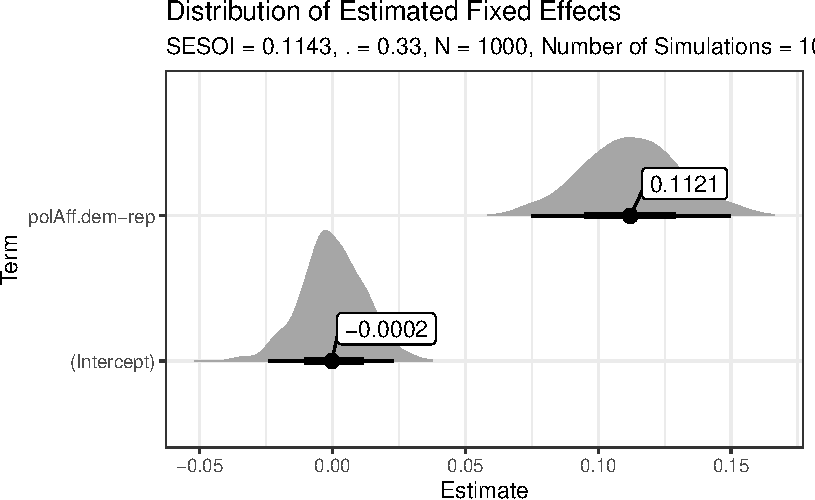
\includegraphics{powerSimulations_files/figure-pdf/fig-checkSims-mainEffect-1.pdf}

}

\subcaption{\label{fig-checkSims-mainEffect}}

}

\caption{\label{fig-checkSims-mainEffect}Distribution of estimated fixed
effects resulting from 1000 simulations for the model deltaDuration
\textasciitilde{} polAff + (1 \textbar{} subj) + (1 \textbar{} trial).
Shaded area represent densities, annotated points indicate medians, and
thick and thin lines represent 66\% and 95\% quantiles.}

\end{figure}%

Figure~\ref{fig-powC-mainEffect} shows results of our sample-size
determination analyses. We find that a sample size of 600 provides a
statistical power of 95.4\% (lower bound of 95\%-CI) even under the most
conservative assumptions (SESOI = 0.1000, Error SD = 0.6600).

We optimize the study design to detect a true SESOI for political
affiliation. However, we are also interested in two-way and three-way
interaction effects, which are known to require greater sample sizes to
achieve the same statistical power as for main effects. Moreover,
greater sample sizes are more likely to accurately represent target
populations with respect to variables like exposure to extreme weather
events and subjective attribution of extreme weather events to climate
change. Therefore, we opt for a sample size of N = 1000 for further
effect-size sensitivity analyses regarding interaction effects.

\begin{figure}

\centering{

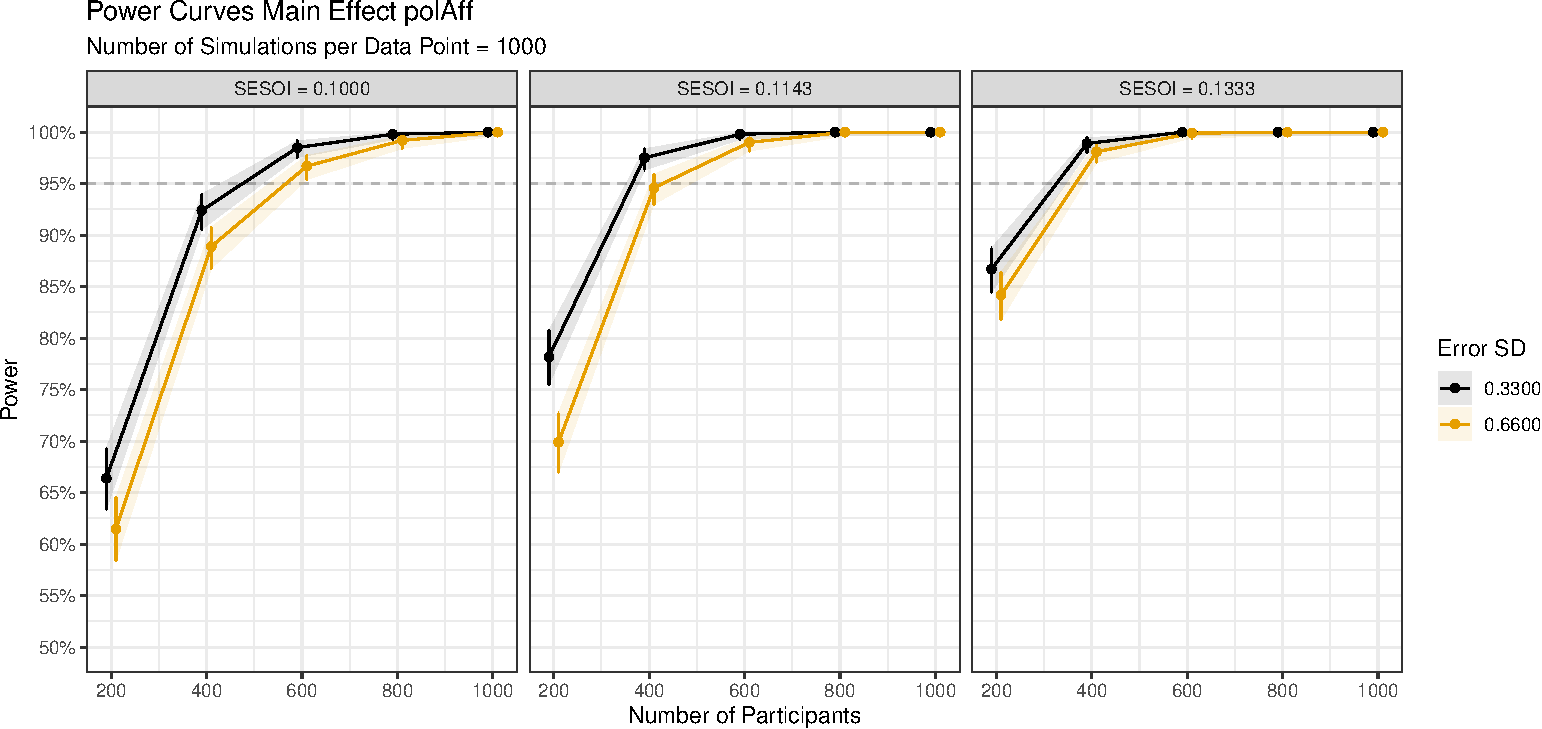
\includegraphics{powerSimulations_files/figure-pdf/fig-powC-mainEffect-1.pdf}

}

\caption{\label{fig-powC-mainEffect}Power curves for the main effect of
polAff. Points represent statistical power surrounded by a 95\%-CI based
on 1000 simulations with α = 0.05.}

\end{figure}%

\section{Two-Way Interaction Effect}\label{two-way-interaction-effect}

As argued in the Registered Report, we hypothesize:

\textbf{(H\textsubscript{2})}: \emph{The effect of political affiliation
on ΔDuration is greater among individuals with prior exposure to extreme
weather events compared to individuals without such exposure. That is,
extreme weather exposure positively interacts with political affiliation
in predicting ΔDuration.}

\begin{Shaded}
\begin{Highlighting}[]
\CommentTok{\# Create a data frame with predicted true effects}

\CommentTok{\# Smallest Effect Size Of Interest (SESOI)}
\NormalTok{SESOI }\OtherTok{\textless{}{-}} \FloatTok{0.4}\SpecialCharTok{/}\FloatTok{3.5}

\CommentTok{\# Betas}
\NormalTok{beta\_p }\OtherTok{\textless{}{-}}\NormalTok{ SESOI}
\NormalTok{beta\_e }\OtherTok{\textless{}{-}} \DecValTok{0}
\NormalTok{beta\_p\_e\_inx }\OtherTok{\textless{}{-}}\NormalTok{ SESOI}

\CommentTok{\# Predicted "true" effects}
\NormalTok{polAff\_ewe\_trueEffects }\OtherTok{\textless{}{-}} \FunctionTok{expand\_grid}\NormalTok{(}
  \AttributeTok{polAff =} \FunctionTok{factor}\NormalTok{(}\FunctionTok{c}\NormalTok{(}\StringTok{"rep"}\NormalTok{, }\StringTok{"dem"}\NormalTok{), }\AttributeTok{levels =} \FunctionTok{c}\NormalTok{(}\StringTok{"rep"}\NormalTok{, }\StringTok{"dem"}\NormalTok{)),}
  \AttributeTok{ewe =} \FunctionTok{factor}\NormalTok{(}\FunctionTok{c}\NormalTok{(}\ConstantTok{FALSE}\NormalTok{, }\ConstantTok{TRUE}\NormalTok{), }\AttributeTok{levels =} \FunctionTok{c}\NormalTok{(}\ConstantTok{FALSE}\NormalTok{, }\ConstantTok{TRUE}\NormalTok{))}
\NormalTok{) }\SpecialCharTok{\%\textgreater{}\%} 
  \FunctionTok{add\_contrast}\NormalTok{(}\StringTok{"polAff"}\NormalTok{, }\AttributeTok{contrast =} \StringTok{"anova"}\NormalTok{, }\AttributeTok{colnames =} \StringTok{"X\_p"}\NormalTok{) }\SpecialCharTok{\%\textgreater{}\%} 
  \FunctionTok{add\_contrast}\NormalTok{(}\StringTok{"ewe"}\NormalTok{, }\AttributeTok{contrast =} \StringTok{"anova"}\NormalTok{, }\AttributeTok{colnames =} \StringTok{"X\_e"}\NormalTok{) }\SpecialCharTok{\%\textgreater{}\%} 
  \FunctionTok{mutate}\NormalTok{(}
    \AttributeTok{trueDeltaDuration =}
      \DecValTok{0} \SpecialCharTok{+}                        \CommentTok{\# intercept}
\NormalTok{      X\_p }\SpecialCharTok{*}\NormalTok{ beta\_p }\SpecialCharTok{+}             \CommentTok{\# main effect polAff}
\NormalTok{      X\_e }\SpecialCharTok{*}\NormalTok{ beta\_e }\SpecialCharTok{+}             \CommentTok{\# main effect ewe}
\NormalTok{      X\_p }\SpecialCharTok{*}\NormalTok{ X\_e }\SpecialCharTok{*}\NormalTok{ beta\_p\_e\_inx   }\CommentTok{\# interaction effect polAff*ewe}
\NormalTok{  )}
\end{Highlighting}
\end{Shaded}

\subsection{SESOI for Two-Way Interaction}\label{sec-SESOI_2wayInt}

For deriving a SESOI for the two-way interaction of interest, similar
considerations apply as in the case of the SESOI for the main effect of
interest. In this section, we make these considerations explicit. We
start by noticing that the complete fixed two-way interaction polAff ×
ewe is modeled as:

\[
\Delta Duration = \beta_{0} + \beta_{1} \cdot polAff + \beta_{2} \cdot ewe  + \beta_{3} \cdot (polAff \times ewe)
\]

By rearranging terms, one can show that the effect of polAff is given
by:

\[
Effect_{polAff} = \beta_{1} + \beta_{3} \cdot ewe
\]

Now, let's calculate this effect for two individuals who differ in their
levels of ewe. As ewe is a binary variable, we have two types of
individuals: individuals with (ewe = 1) and without (ewe = 0) extreme
weather exposure. For an individual without extreme weather exposure,
the effect of polAff will be:

\[
Effect_{noEWE} = \beta_{1} + \beta_{3} \cdot 0 = \beta_{1}
\]

For an individual with extreme weather exposure, the effect of polAff
will be:

\[
Effect_{EWE} = \beta_{1} + \beta_{3} \cdot 1 = \beta_{1} + \beta_{3}
\]

The difference in the effect of polAff between these two individuals is
given by:

\[
\begin{split}
Effect_{EWE} - Effect_{noEWE} = (\beta_{1} + \beta_{3}) - \beta_{1} = \beta_{3}
\end{split}
\]

We consider this difference as theoretically relevant if it is at least
of the same size as the SESOI for the effect of polAff:

\[
SESOI_{polAff \times ewe} = Effect_{EWE} - Effect_{noEWE} = SESOI_{polAff} = 0.1143
\]

\subsection{Data Simulation Function}\label{data-simulation-function-1}

We next define a function that simulates data for the two-way
interaction effect of political affiliation with extreme weather
exposure on ΔDuration: \texttt{FUN\_sim\_2wayInt}. The function will
simulate data according to the following model, expressed in lme4-lingo:

\texttt{deltaDuration\ \textasciitilde{}\ polAff\ *\ ewe\ +\ (1\textbar{}subj)\ +\ (1\textbar{}trial)}

The function \texttt{FUN\_sim\_2wayInt} takes, among others, the
following important arguments (in addition to the arguments discussed
for \texttt{FUN\_sim}):

\begin{itemize}
\item
  \texttt{beta\_p}: \textbf{Fixed main effect of political affiliation}.
  Compatible with H\textsubscript{1}, we keep this value at the SESOI of
  0.1143. That is, we model that the average effect of political
  affiliation across all participants, irrespective of their extreme
  weather exposure, is 0.1143.
\item
  \texttt{beta\_e}: \textbf{Fixed main effect of extreme weather
  exposure}. As we are interested in the moderating role of extreme
  weather exposure, we set this main effect to zero. That is, we assume
  that the effect of extreme weather exposure is highly dependent on
  participants' political affiliation.
\item
  \texttt{beta\_p\_e\_inx}: \textbf{Fixed two-way interaction effect of
  political affiliation and extreme weather exposure}. We set this
  initial value to the SESOI derived above, but we investigate how
  changing this effect size impacts statistical power, as we are
  conducting effect-size sensitivity analyses for interaction effects.
\end{itemize}

The function \texttt{FUN\_sim\_2wayInt} is defined below:

\begin{Shaded}
\begin{Highlighting}[]
\CommentTok{\# define data simulation function}
\NormalTok{FUN\_sim\_2wayInt }\OtherTok{\textless{}{-}} \ControlFlowTok{function}\NormalTok{(}
  \AttributeTok{n\_subj         =}        \DecValTok{1000}\NormalTok{, }\CommentTok{\# number of subjects}
  \AttributeTok{n\_subj\_prop\_p  =}   \FunctionTok{c}\NormalTok{(.}\DecValTok{5}\NormalTok{, .}\DecValTok{5}\NormalTok{), }\CommentTok{\# proportion of republican and democrat subjects}
  \AttributeTok{n\_subj\_prop\_e  =}   \FunctionTok{c}\NormalTok{(.}\DecValTok{5}\NormalTok{, .}\DecValTok{5}\NormalTok{), }\CommentTok{\# proportion of subjects without and with extreme weather exposure}
  \AttributeTok{n\_trial        =}          \DecValTok{25}\NormalTok{, }\CommentTok{\# number of trials}
  \AttributeTok{beta\_0         =}           \DecValTok{0}\NormalTok{, }\CommentTok{\# intercept (grand mean) for deltaDuration}
  \AttributeTok{beta\_p         =}     \FloatTok{0.4}\SpecialCharTok{/}\FloatTok{3.5}\NormalTok{, }\CommentTok{\# main effect of political affiliation (polAff)}
  \AttributeTok{beta\_e         =}           \DecValTok{0}\NormalTok{, }\CommentTok{\# main effect of extreme weather exposure (ewe)}
  \AttributeTok{beta\_p\_e\_inx   =}     \FloatTok{0.4}\SpecialCharTok{/}\FloatTok{3.5}\NormalTok{, }\CommentTok{\# two{-}way interaction effect of polAff and ewe}
  \AttributeTok{subj\_0         =}\NormalTok{         .}\DecValTok{29}\NormalTok{, }\CommentTok{\# by{-}subject random intercept sd for dt carbon}
  \AttributeTok{trial\_0        =}\NormalTok{         .}\DecValTok{04}\NormalTok{, }\CommentTok{\# by{-}trial random intercept sd}
  \AttributeTok{sigma          =} \DecValTok{1}\SpecialCharTok{*}\NormalTok{(.}\DecValTok{29}\FloatTok{+.04}\NormalTok{), }\CommentTok{\# residual (error) sd}
  
  \AttributeTok{truncNums      =}        \ConstantTok{TRUE}\NormalTok{, }\CommentTok{\# should impossible numbers be truncuated?}
  \AttributeTok{setSeed        =}        \ConstantTok{NULL}  \CommentTok{\# seed number to achieve reproducible results. Set to NULL for simulations!}
\NormalTok{) \{}
  
  \CommentTok{\# set seed to achieve reproducible results for demonstration purposes}
  \FunctionTok{set.seed}\NormalTok{(setSeed)}
  
  \CommentTok{\# simulate data for dwell time on carbon information}
\NormalTok{  dataSim }\OtherTok{\textless{}{-}} 
    \CommentTok{\# add random factor subject}
    \FunctionTok{add\_random}\NormalTok{(}\AttributeTok{subj =}\NormalTok{ n\_subj) }\SpecialCharTok{\%\textgreater{}\%} 
    \CommentTok{\# add random factor trial}
    \FunctionTok{add\_random}\NormalTok{(}\AttributeTok{trial =}\NormalTok{ n\_trial) }\SpecialCharTok{\%\textgreater{}\%} 
    \CommentTok{\# add between{-}subject factor political affiliation (with anova contrast)}
    \FunctionTok{add\_between}\NormalTok{(}\StringTok{"subj"}\NormalTok{, }\AttributeTok{polAff =} \FunctionTok{c}\NormalTok{(}\StringTok{"rep"}\NormalTok{, }\StringTok{"dem"}\NormalTok{), }\AttributeTok{.prob =}\NormalTok{ n\_subj\_prop\_p}\SpecialCharTok{*}\NormalTok{n\_subj, }\AttributeTok{.shuffle =} \ConstantTok{TRUE}\NormalTok{) }\SpecialCharTok{\%\textgreater{}\%} 
    \FunctionTok{add\_contrast}\NormalTok{(}\StringTok{"polAff"}\NormalTok{, }\AttributeTok{colnames =} \StringTok{"X\_p"}\NormalTok{, }\AttributeTok{contrast =} \StringTok{"anova"}\NormalTok{) }\SpecialCharTok{\%\textgreater{}\%} 
    \CommentTok{\# add between{-}subject factor extreme weather exposure (with anova contrast)}
    \FunctionTok{add\_between}\NormalTok{(}\StringTok{"subj"}\NormalTok{, }\AttributeTok{ewe =} \FunctionTok{c}\NormalTok{(}\ConstantTok{FALSE}\NormalTok{, }\ConstantTok{TRUE}\NormalTok{), }\AttributeTok{.prob =}\NormalTok{ n\_subj\_prop\_e}\SpecialCharTok{*}\NormalTok{n\_subj, }\AttributeTok{.shuffle =} \ConstantTok{TRUE}\NormalTok{) }\SpecialCharTok{\%\textgreater{}\%} 
    \FunctionTok{add\_contrast}\NormalTok{(}\StringTok{"ewe"}\NormalTok{, }\AttributeTok{colnames =} \StringTok{"X\_e"}\NormalTok{, }\AttributeTok{contrast =} \StringTok{"anova"}\NormalTok{) }\SpecialCharTok{\%\textgreater{}\%} 
    \CommentTok{\# add by{-}subject random intercept}
    \FunctionTok{add\_ranef}\NormalTok{(}\StringTok{"subj"}\NormalTok{, }\AttributeTok{S\_0 =}\NormalTok{ subj\_0) }\SpecialCharTok{\%\textgreater{}\%} 
    \CommentTok{\# add by{-}trial random intercept}
    \FunctionTok{add\_ranef}\NormalTok{(}\StringTok{"trial"}\NormalTok{, }\AttributeTok{T\_0 =}\NormalTok{ trial\_0) }\SpecialCharTok{\%\textgreater{}\%} 
    \CommentTok{\# add error term}
    \FunctionTok{add\_ranef}\NormalTok{(}\AttributeTok{e\_st =}\NormalTok{ sigma) }\SpecialCharTok{\%\textgreater{}\%} 
    \CommentTok{\# add response values}
    \FunctionTok{mutate}\NormalTok{(}
      \CommentTok{\# add together fixed and random effects for each effect}
      \AttributeTok{B\_0 =}\NormalTok{ beta\_0 }\SpecialCharTok{+}\NormalTok{ S\_0 }\SpecialCharTok{+}\NormalTok{ T\_0,}
      \AttributeTok{B\_p =}\NormalTok{ beta\_p,}
      \AttributeTok{B\_e =}\NormalTok{ beta\_e,}
      \AttributeTok{B\_p\_e\_inx =}\NormalTok{ beta\_p\_e\_inx,}
      \CommentTok{\# calculate dv by adding each effect term multiplied by the relevant}
      \CommentTok{\# effect{-}coded factors and adding the error term}
      \AttributeTok{deltaDuration =} 
\NormalTok{        B\_0 }\SpecialCharTok{+}\NormalTok{ e\_st }\SpecialCharTok{+}
\NormalTok{        (X\_p }\SpecialCharTok{*}\NormalTok{ B\_p) }\SpecialCharTok{+}
\NormalTok{        (X\_e }\SpecialCharTok{*}\NormalTok{ B\_e) }\SpecialCharTok{+}
\NormalTok{        (X\_p }\SpecialCharTok{*}\NormalTok{ X\_e }\SpecialCharTok{*}\NormalTok{ B\_p\_e\_inx)}
\NormalTok{    )}
  
  \CommentTok{\# truncuate impossible deltaDurations}
  \ControlFlowTok{if}\NormalTok{(truncNums) \{}
\NormalTok{    dataSim }\OtherTok{\textless{}{-}}\NormalTok{ dataSim }\SpecialCharTok{\%\textgreater{}\%} 
      \FunctionTok{mutate}\NormalTok{(}\AttributeTok{deltaDuration =} \FunctionTok{if\_else}\NormalTok{(deltaDuration }\SpecialCharTok{\textless{}} \SpecialCharTok{{-}}\DecValTok{1}\NormalTok{, }\SpecialCharTok{{-}}\DecValTok{1}\NormalTok{,}
        \FunctionTok{if\_else}\NormalTok{(deltaDuration }\SpecialCharTok{\textgreater{}} \DecValTok{1}\NormalTok{, }\DecValTok{1}\NormalTok{, deltaDuration)))}
\NormalTok{  \}}
  
  \CommentTok{\# run a linear mixed effects model and check summary}
\NormalTok{  mod }\OtherTok{\textless{}{-}} \FunctionTok{lmer}\NormalTok{(}
\NormalTok{    deltaDuration }\SpecialCharTok{\textasciitilde{}}\NormalTok{ polAff}\SpecialCharTok{*}\NormalTok{ewe }\SpecialCharTok{+}\NormalTok{ (}\DecValTok{1} \SpecialCharTok{|}\NormalTok{ subj) }\SpecialCharTok{+}\NormalTok{ (}\DecValTok{1} \SpecialCharTok{|}\NormalTok{ trial),}
    \AttributeTok{data =}\NormalTok{ dataSim}
\NormalTok{  )}
\NormalTok{  mod.sum }\OtherTok{\textless{}{-}} \FunctionTok{summary}\NormalTok{(mod)}
  
  \CommentTok{\# get results in tidy format}
\NormalTok{  mod.broom }\OtherTok{\textless{}{-}}\NormalTok{ broom.mixed}\SpecialCharTok{::}\FunctionTok{tidy}\NormalTok{(mod)}
  
  \FunctionTok{return}\NormalTok{(}\FunctionTok{list}\NormalTok{(}
    \AttributeTok{dataSim =}\NormalTok{ dataSim,}
    \AttributeTok{modelLmer =}\NormalTok{ mod,}
    \AttributeTok{modelResults =}\NormalTok{ mod.broom}
\NormalTok{  ))}
  
\NormalTok{\}}
\end{Highlighting}
\end{Shaded}

We call the function once and extract the results of this single
simulation:

\begin{Shaded}
\begin{Highlighting}[]
\NormalTok{out }\OtherTok{\textless{}{-}} \FunctionTok{FUN\_sim\_2wayInt}\NormalTok{(}
  \AttributeTok{n\_subj         =}        \DecValTok{1000}\NormalTok{, }\CommentTok{\# number of subjects}
  \AttributeTok{n\_subj\_prop\_p  =}   \FunctionTok{c}\NormalTok{(.}\DecValTok{5}\NormalTok{, .}\DecValTok{5}\NormalTok{), }\CommentTok{\# proportion of republican and democrat subjects}
  \AttributeTok{n\_subj\_prop\_e  =}   \FunctionTok{c}\NormalTok{(.}\DecValTok{5}\NormalTok{, .}\DecValTok{5}\NormalTok{), }\CommentTok{\# proportion of subjects without and with extreme weather exposure}
  \AttributeTok{n\_trial        =}          \DecValTok{25}\NormalTok{, }\CommentTok{\# number of trials}
  \AttributeTok{beta\_0         =}           \DecValTok{0}\NormalTok{, }\CommentTok{\# intercept (grand mean) for deltaDuration}
  \AttributeTok{beta\_p         =}     \FloatTok{0.4}\SpecialCharTok{/}\FloatTok{3.5}\NormalTok{, }\CommentTok{\# main effect of political affiliation (polAff)}
  \AttributeTok{beta\_e         =}           \DecValTok{0}\NormalTok{, }\CommentTok{\# main effect of extreme weather exposure (ewe)}
  \AttributeTok{beta\_p\_e\_inx   =}     \FloatTok{0.4}\SpecialCharTok{/}\FloatTok{3.5}\NormalTok{, }\CommentTok{\# two{-}way interaction effect of polAff and ewe}
  \AttributeTok{subj\_0         =}\NormalTok{         .}\DecValTok{29}\NormalTok{, }\CommentTok{\# by{-}subject random intercept sd for dt carbon}
  \AttributeTok{trial\_0        =}\NormalTok{         .}\DecValTok{04}\NormalTok{, }\CommentTok{\# by{-}trial random intercept sd}
  \AttributeTok{sigma          =} \DecValTok{1}\SpecialCharTok{*}\NormalTok{(.}\DecValTok{29}\FloatTok{+.04}\NormalTok{), }\CommentTok{\# residual (error) sd}
  
  \AttributeTok{truncNums      =}        \ConstantTok{TRUE}\NormalTok{, }\CommentTok{\# should impossible numbers be truncuated?}
  \AttributeTok{setSeed        =}        \DecValTok{1234}  \CommentTok{\# seed number to achieve reproducible results. Set to NULL for simulations!}
\NormalTok{)}

\CommentTok{\# Get results table}
\NormalTok{resultsTable }\OtherTok{\textless{}{-}}\NormalTok{ out}\SpecialCharTok{$}\NormalTok{modelResults }\SpecialCharTok{\%\textgreater{}\%} 
  \FunctionTok{select}\NormalTok{(}\SpecialCharTok{{-}}\FunctionTok{c}\NormalTok{(std.error, statistic, df)) }\SpecialCharTok{\%\textgreater{}\%} 
  \FunctionTok{mutate}\NormalTok{(}\FunctionTok{across}\NormalTok{(}\FunctionTok{where}\NormalTok{(is\_double), }\SpecialCharTok{\textasciitilde{}} \FunctionTok{round}\NormalTok{(.x, }\DecValTok{4}\NormalTok{))) }\SpecialCharTok{\%\textgreater{}\%} 
\NormalTok{  knitr}\SpecialCharTok{::}\FunctionTok{kable}\NormalTok{()}
\NormalTok{formulaUsedForFit }\OtherTok{\textless{}{-}} \FunctionTok{paste}\NormalTok{(}\FunctionTok{as.character}\NormalTok{(}\FunctionTok{formula}\NormalTok{(out}\SpecialCharTok{$}\NormalTok{modelLmer))[}\FunctionTok{c}\NormalTok{(}\DecValTok{2}\NormalTok{,}\DecValTok{1}\NormalTok{,}\DecValTok{3}\NormalTok{)], }\AttributeTok{collapse =} \StringTok{" "}\NormalTok{)}

\CommentTok{\# Create plot}
\NormalTok{p.demo}\FloatTok{.2}\NormalTok{wayInt }\OtherTok{\textless{}{-}}\NormalTok{  out}\SpecialCharTok{$}\NormalTok{dataSim }\SpecialCharTok{\%\textgreater{}\%} 
  \FunctionTok{ggplot}\NormalTok{(}\FunctionTok{aes}\NormalTok{(}\AttributeTok{x =}\NormalTok{ ewe, }\AttributeTok{y =}\NormalTok{ deltaDuration, }\AttributeTok{color =}\NormalTok{ polAff)) }\SpecialCharTok{+}
  \FunctionTok{geom\_hline}\NormalTok{(}\AttributeTok{yintercept =} \DecValTok{0}\NormalTok{) }\SpecialCharTok{+}
  \FunctionTok{geom\_violin}\NormalTok{(}\AttributeTok{alpha =} \FloatTok{0.3}\NormalTok{) }\SpecialCharTok{+}
  \FunctionTok{geom\_point}\NormalTok{(}
    \AttributeTok{data =}\NormalTok{ polAff\_ewe\_trueEffects,}
    \AttributeTok{mapping =} \FunctionTok{aes}\NormalTok{(}\AttributeTok{x =}\NormalTok{ ewe, }\AttributeTok{y =}\NormalTok{ trueDeltaDuration, }\AttributeTok{fill =}\NormalTok{ polAff),}
    \AttributeTok{shape =} \StringTok{"circle open"}\NormalTok{,}
    \AttributeTok{size =} \FloatTok{3.5}\NormalTok{,}
    \AttributeTok{stroke =} \DecValTok{2}\NormalTok{,}
    \AttributeTok{color =} \StringTok{"black"}\NormalTok{,}
    \AttributeTok{position =} \FunctionTok{position\_dodge}\NormalTok{(}\AttributeTok{width =}\NormalTok{ .}\DecValTok{9}\NormalTok{),}
    \AttributeTok{show.legend =} \ConstantTok{FALSE}
\NormalTok{  ) }\SpecialCharTok{+}
  \FunctionTok{stat\_summary}\NormalTok{(}
    \AttributeTok{fun =}\NormalTok{ mean,}
    \AttributeTok{fun.min =}\NormalTok{ \textbackslash{}(x)\{}\FunctionTok{mean}\NormalTok{(x) }\SpecialCharTok{{-}} \FunctionTok{sd}\NormalTok{(x)\},}
    \AttributeTok{fun.max =}\NormalTok{ \textbackslash{}(x)\{}\FunctionTok{mean}\NormalTok{(x) }\SpecialCharTok{+} \FunctionTok{sd}\NormalTok{(x)\},}
    \AttributeTok{position =} \FunctionTok{position\_dodge}\NormalTok{(}\AttributeTok{width =}\NormalTok{ .}\DecValTok{9}\NormalTok{)}
\NormalTok{  ) }\SpecialCharTok{+}
\NormalTok{  ggrepel}\SpecialCharTok{::}\FunctionTok{geom\_label\_repel}\NormalTok{(}
    \AttributeTok{data =}\NormalTok{ polAff\_ewe\_trueEffects,}
    \AttributeTok{mapping =} \FunctionTok{aes}\NormalTok{(}\AttributeTok{x =}\NormalTok{ ewe, }\AttributeTok{y =}\NormalTok{ trueDeltaDuration, }\AttributeTok{fill =}\NormalTok{ polAff, }\AttributeTok{label =} \FunctionTok{round}\NormalTok{(trueDeltaDuration, }\DecValTok{4}\NormalTok{)),}
    \AttributeTok{color =} \StringTok{"black"}\NormalTok{,}
    \AttributeTok{box.padding =} \DecValTok{1}\NormalTok{,}
    \AttributeTok{position =} \FunctionTok{position\_dodge}\NormalTok{(}\AttributeTok{width =}\NormalTok{ .}\DecValTok{9}\NormalTok{),}
    \AttributeTok{show.legend =} \ConstantTok{FALSE}
\NormalTok{  ) }\SpecialCharTok{+}
  \FunctionTok{scale\_color\_manual}\NormalTok{(}\AttributeTok{values =} \FunctionTok{c}\NormalTok{(}\StringTok{"red"}\NormalTok{, }\StringTok{"dodgerblue"}\NormalTok{)) }\SpecialCharTok{+}
  \FunctionTok{scale\_fill\_manual}\NormalTok{(}\AttributeTok{values =} \FunctionTok{c}\NormalTok{(}\StringTok{"white"}\NormalTok{, }\StringTok{"white"}\NormalTok{)) }\SpecialCharTok{+}
  \FunctionTok{scale\_y\_continuous}\NormalTok{(}\AttributeTok{breaks =} \FunctionTok{seq}\NormalTok{(}\SpecialCharTok{{-}}\DecValTok{1}\NormalTok{, }\DecValTok{1}\NormalTok{, .}\DecValTok{2}\NormalTok{)) }\SpecialCharTok{+}
  \FunctionTok{labs}\NormalTok{(}\AttributeTok{title =} \StringTok{"Demo Output of One Simulation for Two{-}Way Interaction"}\NormalTok{) }\SpecialCharTok{+}
  \FunctionTok{theme\_bw}\NormalTok{()}
\end{Highlighting}
\end{Shaded}

Figure~\ref{fig-demoFUNSim_2wayInt} visualizes the results of this
single simulation and Table~\ref{tbl-demoFUNSim_2wayInt} summarizes the
statistical results of fitting the actual model used in data generation
to the simulated data.

\begin{figure}

\centering{

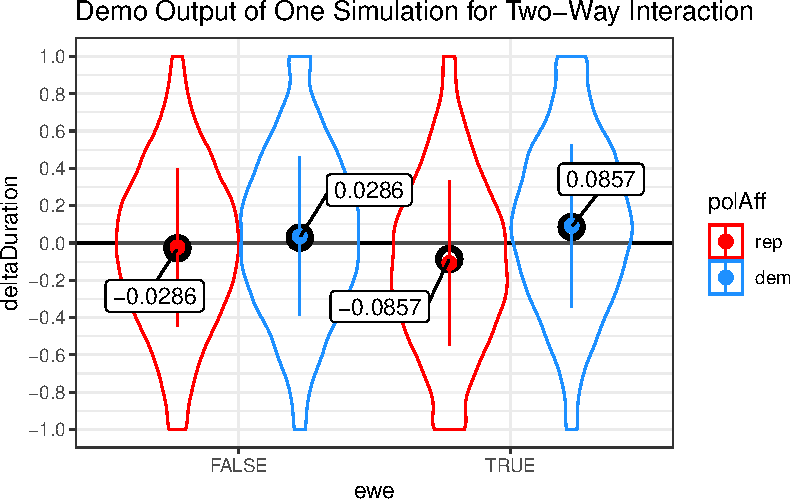
\includegraphics{powerSimulations_files/figure-pdf/fig-demoFUNSim_2wayInt-1.pdf}

}

\caption{\label{fig-demoFUNSim_2wayInt}Visual representation of results
of one simulation created using \texttt{FUN\_sim\_2wayInt}. Violin plots
display the full distribution of the data. Points and surrounding lines
indicate the mean ± 1 SD. The black horizontal line displays the true
sample mean and the black open circles indicate the true means for each
cell.}

\end{figure}%

\phantomsection\label{tbl-demoFUNSim_2wayInt}
\begin{longtable}[]{@{}lllrr@{}}

\caption{\label{tbl-demoFUNSim_2wayInt}Statistical results of one
simulation created using \texttt{FUN\_sim\_2wayInt}. Data was fit using
deltaDuration \textasciitilde{} polAff * ewe + (1 \textbar{} subj) + (1
\textbar{} trial).}

\tabularnewline

\toprule\noalign{}
effect & group & term & estimate & p.value \\
\midrule\noalign{}
\endhead
\bottomrule\noalign{}
\endlastfoot
fixed & NA & (Intercept) & -0.0006 & 0.9625 \\
fixed & NA & polAff.dem-rep & 0.1290 & 0.0000 \\
fixed & NA & ewe.TRUE-FALSE & -0.0139 & 0.4516 \\
fixed & NA & polAff.dem-rep:ewe.TRUE-FALSE & 0.1398 & 0.0002 \\
ran\_pars & subj & sd\_\_(Intercept) & 0.2855 & NA \\
ran\_pars & trial & sd\_\_(Intercept) & 0.0382 & NA \\
ran\_pars & Residual & sd\_\_Observation & 0.3232 & NA \\

\end{longtable}

\subsection{Power Simulation}\label{power-simulation-1}

In the following code, the simulations are calculated. We do not
recommend executing this code junk as it takes several hours to run.

\begin{Shaded}
\begin{Highlighting}[]
\NormalTok{FUN\_sim\_2wayInt\_pwr }\OtherTok{\textless{}{-}} \ControlFlowTok{function}\NormalTok{(sim, ...)\{}
\NormalTok{  out }\OtherTok{\textless{}{-}} \FunctionTok{FUN\_sim\_2wayInt}\NormalTok{(...)}
\NormalTok{  modelResults }\OtherTok{\textless{}{-}}\NormalTok{ out}\SpecialCharTok{$}\NormalTok{modelResults }\SpecialCharTok{\%\textgreater{}\%} 
    \FunctionTok{mutate}\NormalTok{(}\AttributeTok{sim =}\NormalTok{ sim) }\SpecialCharTok{\%\textgreater{}\%} 
    \FunctionTok{relocate}\NormalTok{(sim)}
  \FunctionTok{return}\NormalTok{(modelResults)}
\NormalTok{\}}

\CommentTok{\# How many simulations should be run?}
\NormalTok{n\_sims }\OtherTok{\textless{}{-}} \DecValTok{1000}

\CommentTok{\# What are the breaks for number of subjects we would like to calculate power for?}
\NormalTok{breaks\_subj }\OtherTok{\textless{}{-}} \FunctionTok{c}\NormalTok{(}\DecValTok{900}\NormalTok{, }\DecValTok{950}\NormalTok{, }\DecValTok{1000}\NormalTok{)}

\CommentTok{\# What are the breaks for SESOI?}
\NormalTok{breaks\_sesoi }\OtherTok{\textless{}{-}}\NormalTok{ (}\FloatTok{0.4}\SpecialCharTok{/}\FloatTok{3.5}\NormalTok{)}\SpecialCharTok{*}\FunctionTok{seq}\NormalTok{(}\DecValTok{1}\NormalTok{, }\DecValTok{2}\NormalTok{, .}\DecValTok{25}\NormalTok{)}

\CommentTok{\# What are the breaks for different error SDs?}
\NormalTok{breaks\_sigma }\OtherTok{\textless{}{-}} \FunctionTok{c}\NormalTok{((.}\DecValTok{29}\FloatTok{+.04}\NormalTok{), }\DecValTok{2}\SpecialCharTok{*}\NormalTok{(.}\DecValTok{29}\FloatTok{+.04}\NormalTok{))}

\NormalTok{res\_2wayInt }\OtherTok{\textless{}{-}} \FunctionTok{tibble}\NormalTok{()}
\ControlFlowTok{for}\NormalTok{ (s }\ControlFlowTok{in} \FunctionTok{seq\_along}\NormalTok{(breaks\_sigma)) \{}
  
\NormalTok{  res\_sesoi }\OtherTok{\textless{}{-}} \FunctionTok{tibble}\NormalTok{()}
  \ControlFlowTok{for}\NormalTok{ (sesoi }\ControlFlowTok{in} \FunctionTok{seq\_along}\NormalTok{(breaks\_sesoi)) \{}
    
\NormalTok{    res\_nSubj }\OtherTok{\textless{}{-}} \FunctionTok{tibble}\NormalTok{()}
    \ControlFlowTok{for}\NormalTok{ (nSubj }\ControlFlowTok{in} \FunctionTok{seq\_along}\NormalTok{(breaks\_subj)) \{}
      
      \CommentTok{\# Give feedback regarding which model is simulated}
      \FunctionTok{cat}\NormalTok{(}\FunctionTok{paste0}\NormalTok{(}
        \StringTok{"Simulation:}\SpecialCharTok{\textbackslash{}n}\StringTok{"}\NormalTok{,}
        \StringTok{"  sigma = "}\NormalTok{, }\FunctionTok{round}\NormalTok{(breaks\_sigma[s], }\DecValTok{4}\NormalTok{), }\StringTok{"}\SpecialCharTok{\textbackslash{}n}\StringTok{"}\NormalTok{,}
        \StringTok{"  sesoi = "}\NormalTok{, }\FunctionTok{round}\NormalTok{(breaks\_sesoi[sesoi], }\DecValTok{4}\NormalTok{), }\StringTok{"}\SpecialCharTok{\textbackslash{}n}\StringTok{"}\NormalTok{,}
        \StringTok{"  nSubject = "}\NormalTok{, breaks\_subj[nSubj], }\StringTok{"}\SpecialCharTok{\textbackslash{}n}\StringTok{"}
\NormalTok{      ))}
      
      \CommentTok{\# Start timer}
      \FunctionTok{cat}\NormalTok{(}\FunctionTok{paste0}\NormalTok{(}\StringTok{"Start date time: "}\NormalTok{, lubridate}\SpecialCharTok{::}\FunctionTok{now}\NormalTok{(), }\StringTok{"}\SpecialCharTok{\textbackslash{}n}\StringTok{"}\NormalTok{))}
      \FunctionTok{tic}\NormalTok{()}
      
      \CommentTok{\# Loop over simulations}
\NormalTok{      pwr }\OtherTok{\textless{}{-}} \FunctionTok{map\_df}\NormalTok{(}
        \DecValTok{1}\SpecialCharTok{:}\NormalTok{n\_sims, }
\NormalTok{        FUN\_sim\_2wayInt\_pwr,}
        \AttributeTok{n\_subj =}\NormalTok{ breaks\_subj[nSubj],}
        \AttributeTok{beta\_p\_e\_inx =}\NormalTok{ breaks\_sesoi[sesoi],}
        \AttributeTok{sigma =}\NormalTok{ breaks\_sigma[s]}
\NormalTok{      )}
      
      \CommentTok{\# Stop timer and calculate elapsed time}
\NormalTok{      elapsed\_time }\OtherTok{\textless{}{-}} \FunctionTok{toc}\NormalTok{(}\AttributeTok{quiet =} \ConstantTok{TRUE}\NormalTok{)}
\NormalTok{      elapsed\_seconds }\OtherTok{\textless{}{-}}\NormalTok{ elapsed\_time}\SpecialCharTok{$}\NormalTok{toc }\SpecialCharTok{{-}}\NormalTok{ elapsed\_time}\SpecialCharTok{$}\NormalTok{tic}
\NormalTok{      elapsed\_minutes }\OtherTok{\textless{}{-}}\NormalTok{ elapsed\_seconds }\SpecialCharTok{/} \DecValTok{60}
      \FunctionTok{cat}\NormalTok{(}\FunctionTok{paste0}\NormalTok{(}\StringTok{"End date time: "}\NormalTok{, lubridate}\SpecialCharTok{::}\FunctionTok{now}\NormalTok{(), }\StringTok{"}\SpecialCharTok{\textbackslash{}n}\StringTok{"}\NormalTok{))}
      \FunctionTok{cat}\NormalTok{(}\StringTok{"Elapsed time: "}\NormalTok{, elapsed\_minutes, }\StringTok{" minutes}\SpecialCharTok{\textbackslash{}n\textbackslash{}n}\StringTok{"}\NormalTok{)}
      
      \CommentTok{\# Add number of subjects to pwr}
\NormalTok{      pwr }\OtherTok{\textless{}{-}}\NormalTok{ pwr }\SpecialCharTok{\%\textgreater{}\%} 
        \FunctionTok{mutate}\NormalTok{(}
          \AttributeTok{nSubjects =}\NormalTok{ breaks\_subj[nSubj],}
          \AttributeTok{sesoi =}\NormalTok{ breaks\_sesoi[sesoi],}
          \AttributeTok{sigma =}\NormalTok{ breaks\_sigma[s]}
\NormalTok{        )}
      
      \CommentTok{\# Add results to the results table}
\NormalTok{      res\_nSubj }\OtherTok{\textless{}{-}}\NormalTok{ res\_nSubj }\SpecialCharTok{\%\textgreater{}\%}
        \FunctionTok{rbind}\NormalTok{(pwr)}
\NormalTok{    \}}
    
    \CommentTok{\# Add results to the results table}
\NormalTok{    res\_sesoi }\OtherTok{\textless{}{-}}\NormalTok{ res\_sesoi }\SpecialCharTok{\%\textgreater{}\%} 
      \FunctionTok{rbind}\NormalTok{(res\_nSubj)}
\NormalTok{  \}}
  
  \CommentTok{\# Add results to the results table}
\NormalTok{  res\_2wayInt }\OtherTok{\textless{}{-}}\NormalTok{ res\_2wayInt }\SpecialCharTok{\%\textgreater{}\%} 
    \FunctionTok{rbind}\NormalTok{(res\_sesoi)}
  
\NormalTok{\}}

\NormalTok{res\_2wayInt.summary }\OtherTok{\textless{}{-}}\NormalTok{ res\_2wayInt }\SpecialCharTok{\%\textgreater{}\%} 
  \FunctionTok{filter}\NormalTok{(term }\SpecialCharTok{==} \StringTok{"polAff.dem{-}rep:ewe.TRUE{-}FALSE"}\NormalTok{) }\SpecialCharTok{\%\textgreater{}\%} 
  \FunctionTok{group\_by}\NormalTok{(sigma, sesoi, nSubjects) }\SpecialCharTok{\%\textgreater{}\%} 
  \FunctionTok{summarise}\NormalTok{(}
    \AttributeTok{power =} \FunctionTok{mean}\NormalTok{(p.value }\SpecialCharTok{\textless{}} \FloatTok{0.05}\NormalTok{),}
    \AttributeTok{ci.lower =} \FunctionTok{binom.confint}\NormalTok{(power}\SpecialCharTok{*}\NormalTok{n\_sims, n\_sims, }\AttributeTok{methods =} \StringTok{"exact"}\NormalTok{)}\SpecialCharTok{$}\NormalTok{lower,}
    \AttributeTok{ci.upper =} \FunctionTok{binom.confint}\NormalTok{(power}\SpecialCharTok{*}\NormalTok{n\_sims, n\_sims, }\AttributeTok{methods =} \StringTok{"exact"}\NormalTok{)}\SpecialCharTok{$}\NormalTok{upper,}
    \AttributeTok{.groups =} \StringTok{\textquotesingle{}drop\textquotesingle{}}
\NormalTok{  ) }\SpecialCharTok{\%\textgreater{}\%} 
  \FunctionTok{mutate}\NormalTok{(}
    \AttributeTok{sigma\_fact =} \FunctionTok{factor}\NormalTok{(}\FunctionTok{format}\NormalTok{(}\FunctionTok{round}\NormalTok{(sigma, }\DecValTok{4}\NormalTok{), }\AttributeTok{nsmall =} \DecValTok{4}\NormalTok{)),}
    \AttributeTok{sigma\_level =} \FunctionTok{match}\NormalTok{(sigma\_fact, }\FunctionTok{levels}\NormalTok{(sigma\_fact)),}
    \AttributeTok{sesoi\_fact =} \FunctionTok{factor}\NormalTok{(}\FunctionTok{format}\NormalTok{(}\FunctionTok{round}\NormalTok{(sesoi, }\DecValTok{4}\NormalTok{), }\AttributeTok{nsmall =} \DecValTok{4}\NormalTok{)),}
    \AttributeTok{sesoi\_level =} \FunctionTok{match}\NormalTok{(sesoi\_fact, }\FunctionTok{levels}\NormalTok{(sesoi\_fact))}
\NormalTok{  )}

\CommentTok{\# Save results in a list object}
\NormalTok{time }\OtherTok{\textless{}{-}} \FunctionTok{format}\NormalTok{(}\FunctionTok{Sys.time}\NormalTok{(), }\StringTok{"\%Y\%m\%d\_\%H\%M"}\NormalTok{)}
\NormalTok{fileName }\OtherTok{\textless{}{-}} \FunctionTok{paste0}\NormalTok{(}\StringTok{"res\_2wayInt"}\NormalTok{, }\StringTok{"\_"}\NormalTok{, time, }\StringTok{".RDS"}\NormalTok{)}
\FunctionTok{saveRDS}\NormalTok{(}
  \FunctionTok{list}\NormalTok{(}
    \AttributeTok{res\_2wayInt =}\NormalTok{ res\_2wayInt,}
    \AttributeTok{res\_2wayInt.summary =}\NormalTok{ res\_2wayInt.summary}
\NormalTok{  ),}
  \AttributeTok{file =} \FunctionTok{file.path}\NormalTok{(}\StringTok{"../powerSimulationsOutput"}\NormalTok{, fileName)}
\NormalTok{)}
\end{Highlighting}
\end{Shaded}

We retrieve pre-run results:

\begin{Shaded}
\begin{Highlighting}[]
\CommentTok{\# Load power simulation data}
\NormalTok{resList\_2wayInt }\OtherTok{\textless{}{-}} \FunctionTok{readRDS}\NormalTok{(}\FunctionTok{file.path}\NormalTok{(}\StringTok{"../powerSimulationsOutput"}\NormalTok{, }\StringTok{"res\_2wayInt\_20240814\_1052.RDS"}\NormalTok{))}
\NormalTok{resList\_2wayInt.summary }\OtherTok{\textless{}{-}}\NormalTok{ resList\_2wayInt}\SpecialCharTok{$}\NormalTok{res\_2wayInt.summary}

\CommentTok{\# Extract power values for some specific assumptions}
\NormalTok{chosenN }\OtherTok{\textless{}{-}} \DecValTok{950}
\NormalTok{chosenSigma }\OtherTok{\textless{}{-}} \FunctionTok{c}\NormalTok{(}\StringTok{"0.3300"}\NormalTok{, }\StringTok{"0.6600"}\NormalTok{)}
\NormalTok{chosenSESOI }\OtherTok{\textless{}{-}} \FunctionTok{c}\NormalTok{(}\StringTok{"0.1429"}\NormalTok{, }\StringTok{"0.1714"}\NormalTok{)}
\NormalTok{powerValues }\OtherTok{\textless{}{-}}\NormalTok{ resList\_2wayInt.summary }\SpecialCharTok{\%\textgreater{}\%} 
  \FunctionTok{filter}\NormalTok{(sigma\_fact }\SpecialCharTok{\%in\%}\NormalTok{ chosenSigma) }\SpecialCharTok{\%\textgreater{}\%} 
  \FunctionTok{filter}\NormalTok{(sesoi\_fact }\SpecialCharTok{\%in\%}\NormalTok{ chosenSESOI) }\SpecialCharTok{\%\textgreater{}\%} 
  \FunctionTok{filter}\NormalTok{(nSubjects }\SpecialCharTok{\%in\%}\NormalTok{ chosenN) }\SpecialCharTok{\%\textgreater{}\%} 
  \FunctionTok{mutate}\NormalTok{(}\AttributeTok{power\_str =} \FunctionTok{paste0}\NormalTok{(}\FunctionTok{round}\NormalTok{(power}\SpecialCharTok{*}\DecValTok{100}\NormalTok{, }\DecValTok{2}\NormalTok{), }\StringTok{"\%"}\NormalTok{)) }\SpecialCharTok{\%\textgreater{}\%} 
  \FunctionTok{pull}\NormalTok{(power\_str)}

\CommentTok{\# Extract number of simulations}
\NormalTok{label\_nSimulations }\OtherTok{\textless{}{-}}\NormalTok{ resList\_2wayInt}\SpecialCharTok{$}\NormalTok{res\_2wayInt}\SpecialCharTok{$}\NormalTok{sim }\SpecialCharTok{\%\textgreater{}\%} \FunctionTok{n\_distinct}\NormalTok{()}

\CommentTok{\# Repeat breaks\_sesoi}
\NormalTok{breaks\_sesoi }\OtherTok{\textless{}{-}}\NormalTok{ (}\FloatTok{0.4}\SpecialCharTok{/}\FloatTok{3.5}\NormalTok{)}\SpecialCharTok{*}\FunctionTok{seq}\NormalTok{(}\DecValTok{1}\NormalTok{, }\DecValTok{2}\NormalTok{, .}\DecValTok{25}\NormalTok{)}
\end{Highlighting}
\end{Shaded}

Figure~\ref{fig-checkSims-twoWayInt} displays the distribution of
estimated fixed effects across all simulations. The figure shows that
the estimated fixed effects are close to the true ones provided as input
in the data simulation function, validating that simulations worked as
expected.

\begin{figure}[H]

\centering{

\begin{Shaded}
\begin{Highlighting}[]
\CommentTok{\# Define some filters }
\NormalTok{filter\_nSubjects }\OtherTok{\textless{}{-}} \DecValTok{1000}
\NormalTok{filter\_sesoi }\OtherTok{\textless{}{-}} \FunctionTok{unique}\NormalTok{(resList\_2wayInt}\SpecialCharTok{$}\NormalTok{res\_2wayInt}\SpecialCharTok{$}\NormalTok{sesoi)[}\DecValTok{1}\NormalTok{]}
\NormalTok{filter\_sigma }\OtherTok{\textless{}{-}} \FunctionTok{unique}\NormalTok{(resList\_2wayInt}\SpecialCharTok{$}\NormalTok{res\_2wayInt}\SpecialCharTok{$}\NormalTok{sigma)[}\DecValTok{1}\NormalTok{]}

\CommentTok{\# Prepare data for plot}
\NormalTok{fixedEstimates }\OtherTok{\textless{}{-}}\NormalTok{ resList\_2wayInt}\SpecialCharTok{$}\NormalTok{res\_2wayInt }\SpecialCharTok{\%\textgreater{}\%} 
  \FunctionTok{mutate}\NormalTok{(}
    \AttributeTok{group =} \FunctionTok{ifelse}\NormalTok{(}\FunctionTok{is.na}\NormalTok{(group), }\StringTok{""}\NormalTok{, group),}
    \AttributeTok{group\_term =} \FunctionTok{str\_remove}\NormalTok{(}\FunctionTok{str\_c}\NormalTok{(group, term, }\AttributeTok{sep =} \StringTok{"\_"}\NormalTok{), }\StringTok{"\^{}\_"}\NormalTok{)}
\NormalTok{  ) }\SpecialCharTok{\%\textgreater{}\%} 
  \FunctionTok{filter}\NormalTok{(effect }\SpecialCharTok{==} \StringTok{"fixed"}\NormalTok{) }\SpecialCharTok{\%\textgreater{}\%} 
  \FunctionTok{filter}\NormalTok{(nSubjects }\SpecialCharTok{==}\NormalTok{ filter\_nSubjects) }\SpecialCharTok{\%\textgreater{}\%} 
  \FunctionTok{filter}\NormalTok{(sesoi }\SpecialCharTok{==}\NormalTok{ filter\_sesoi) }\SpecialCharTok{\%\textgreater{}\%} 
  \FunctionTok{filter}\NormalTok{(sigma }\SpecialCharTok{==}\NormalTok{ filter\_sigma)}
\NormalTok{fixedEstimates\_medians }\OtherTok{\textless{}{-}}\NormalTok{ fixedEstimates }\SpecialCharTok{\%\textgreater{}\%} 
  \FunctionTok{group\_by}\NormalTok{(group\_term) }\SpecialCharTok{\%\textgreater{}\%} 
  \FunctionTok{summarise}\NormalTok{(}
    \AttributeTok{median =} \FunctionTok{median}\NormalTok{(estimate, }\AttributeTok{na.rm =} \ConstantTok{TRUE}\NormalTok{),}
    \AttributeTok{median\_rounded =} \FunctionTok{format}\NormalTok{(}\FunctionTok{round}\NormalTok{(median, }\DecValTok{4}\NormalTok{), }\AttributeTok{nsmall =} \DecValTok{4}\NormalTok{, }\AttributeTok{scientific =} \ConstantTok{FALSE}\NormalTok{),}
    \AttributeTok{.groups =} \StringTok{\textquotesingle{}drop\textquotesingle{}}
\NormalTok{  )}

\CommentTok{\# Create plot}
\NormalTok{p.checkSims}\FloatTok{.2}\NormalTok{wayInt }\OtherTok{\textless{}{-}}\NormalTok{fixedEstimates }\SpecialCharTok{\%\textgreater{}\%} 
  \FunctionTok{ggplot}\NormalTok{(}\FunctionTok{aes}\NormalTok{(}\AttributeTok{x =}\NormalTok{ estimate, }\AttributeTok{y =}\NormalTok{ group\_term)) }\SpecialCharTok{+}
\NormalTok{  ggdist}\SpecialCharTok{::}\FunctionTok{stat\_halfeye}\NormalTok{() }\SpecialCharTok{+}
\NormalTok{  ggrepel}\SpecialCharTok{::}\FunctionTok{geom\_label\_repel}\NormalTok{(}
    \AttributeTok{data =}\NormalTok{ fixedEstimates\_medians,}
    \AttributeTok{mapping =} \FunctionTok{aes}\NormalTok{(}\AttributeTok{x =}\NormalTok{ median, }\AttributeTok{y =}\NormalTok{ group\_term, }\AttributeTok{label =}\NormalTok{ median\_rounded),}
    \AttributeTok{box.padding =}\NormalTok{ .}\DecValTok{5}
\NormalTok{  ) }\SpecialCharTok{+}
  \FunctionTok{labs}\NormalTok{(}
    \AttributeTok{title =} \StringTok{"Distribution of Estimated Fixed Effects"}\NormalTok{,}
    \AttributeTok{subtitle =} \FunctionTok{paste0}\NormalTok{(}
      \StringTok{"SESOI = "}\NormalTok{, }\FunctionTok{round}\NormalTok{(filter\_sesoi, }\DecValTok{4}\NormalTok{), }\StringTok{", "}\NormalTok{,}
      \StringTok{"σ = "}\NormalTok{, }\FunctionTok{round}\NormalTok{(filter\_sigma, }\DecValTok{4}\NormalTok{), }\StringTok{", "}\NormalTok{,}
      \StringTok{"N = "}\NormalTok{, filter\_nSubjects, }\StringTok{", "}\NormalTok{,}
      \StringTok{"Number of Simulations = "}\NormalTok{, label\_nSimulations}
\NormalTok{    ),}
    \AttributeTok{x =} \StringTok{"Estimate"}\NormalTok{,}
    \AttributeTok{y =} \StringTok{"Term"}
\NormalTok{  ) }\SpecialCharTok{+}
  \FunctionTok{theme\_bw}\NormalTok{()}

\FunctionTok{print}\NormalTok{(p.checkSims}\FloatTok{.2}\NormalTok{wayInt)}
\end{Highlighting}
\end{Shaded}

\centering{

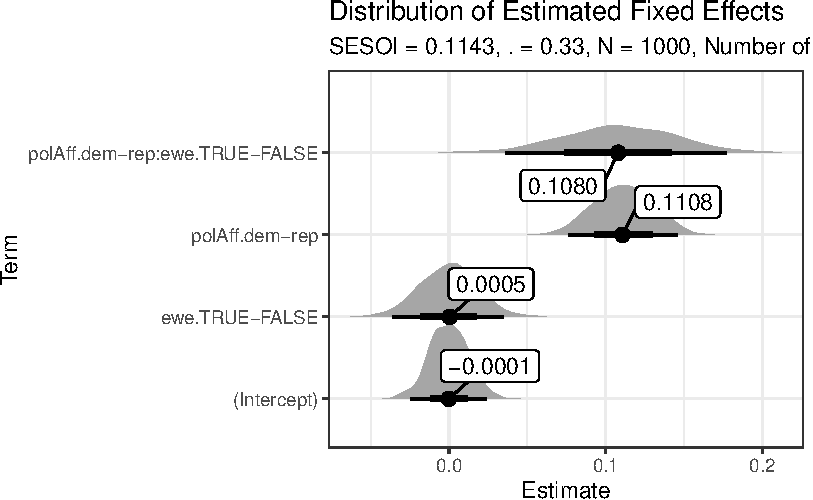
\includegraphics{powerSimulations_files/figure-pdf/fig-checkSims-twoWayInt-1.pdf}

}

\subcaption{\label{fig-checkSims-twoWayInt}}

}

\caption{\label{fig-checkSims-twoWayInt}Distribution of estimated fixed
effects resulting from 1000 simulations for the model deltaDuration
\textasciitilde{} polAff * ewe + (1 \textbar{} subj) + (1 \textbar{}
trial). Shaded area represent densities, annotated points indicate
medians, and thick and thin lines represent 66\% and 95\% quantiles.}

\end{figure}%

Figure~\ref{fig-powC-twoWayInt} shows results of our effect-size
sensitivity analyses. We plot statistical power (y-axis) for different
effect sizes (x-axis), taking into account different assumptions for the
error SD (color) and sample size (panel). Regarding the latter, we
report results not only for the full sample size we aim for (N = 1000),
but also for sample sizes taking into account different participant
exclusion-rates due to exclusion criteria defined in the Registered
Report.

\begin{figure}

\centering{

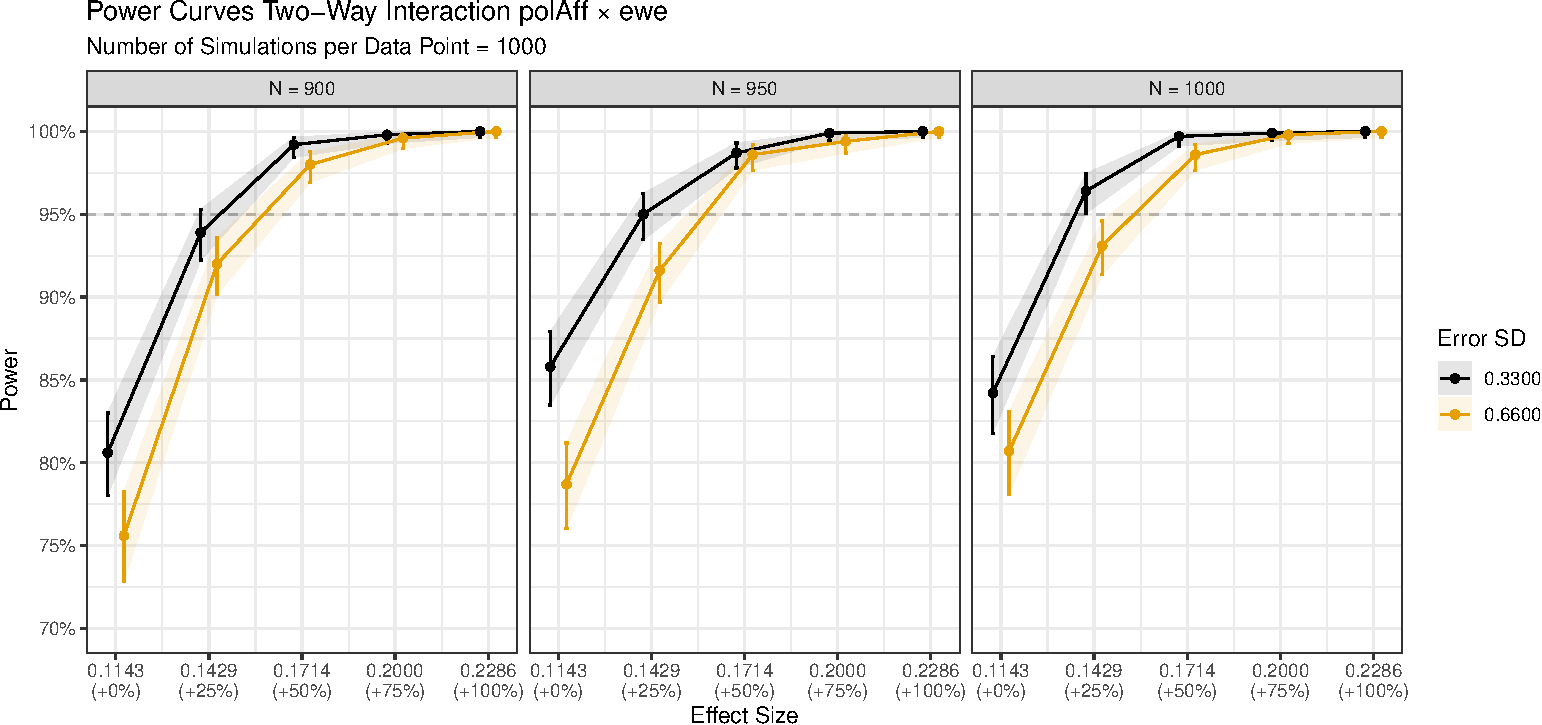
\includegraphics{powerSimulations_files/figure-pdf/fig-powC-twoWayInt-1.pdf}

}

\caption{\label{fig-powC-twoWayInt}Power curves for the two-way
interaction polAff × ewe. Points represent simulated power surrounded by
a 95\%-CI based on 1000 simulations with α = 0.05. Note that, in
contrast to Figure~\ref{fig-powC-mainEffect}, the x-axsis represents
different effect sizes, starting from the defined SESOI, while the
panels represent different sample sizes, taking into account participant
exclusion-rates of 10\% (N = 900), 5\% (N = 950), and 0\% (N = 1000).
Note that estimates are displayed with a slight shift along the x-axis
to reduce overlap.}

\end{figure}%

\begin{Shaded}
\begin{Highlighting}[]
\CommentTok{\# Get power values of interest}
\NormalTok{chosenN }\OtherTok{\textless{}{-}} \DecValTok{950}
\NormalTok{chosenSigma }\OtherTok{\textless{}{-}} \FunctionTok{c}\NormalTok{(}\StringTok{"0.3300"}\NormalTok{, }\StringTok{"0.6600"}\NormalTok{)}
\NormalTok{chosenSESOI }\OtherTok{\textless{}{-}} \FunctionTok{c}\NormalTok{(}\StringTok{"0.1429"}\NormalTok{, }\StringTok{"0.1714"}\NormalTok{)}
\NormalTok{powerValues }\OtherTok{\textless{}{-}}\NormalTok{ resList\_2wayInt.summary }\SpecialCharTok{\%\textgreater{}\%} 
  \FunctionTok{filter}\NormalTok{(sigma\_fact }\SpecialCharTok{\%in\%}\NormalTok{ chosenSigma) }\SpecialCharTok{\%\textgreater{}\%} 
  \FunctionTok{filter}\NormalTok{(sesoi\_fact }\SpecialCharTok{\%in\%}\NormalTok{ chosenSESOI) }\SpecialCharTok{\%\textgreater{}\%} 
  \FunctionTok{filter}\NormalTok{(nSubjects }\SpecialCharTok{\%in\%}\NormalTok{ chosenN)}

\CommentTok{\# Get lower CI for power values for more liberal and more conservative sigma assumptions}
\NormalTok{powerValues\_sigmaLib }\OtherTok{\textless{}{-}}\NormalTok{ powerValues }\SpecialCharTok{\%\textgreater{}\%} 
  \FunctionTok{filter}\NormalTok{(sigma\_fact }\SpecialCharTok{==} \StringTok{"0.3300"}\NormalTok{)}
\NormalTok{powerValues\_sigmaCons }\OtherTok{\textless{}{-}}\NormalTok{ powerValues }\SpecialCharTok{\%\textgreater{}\%} 
  \FunctionTok{filter}\NormalTok{(sigma\_fact }\SpecialCharTok{==} \StringTok{"0.6600"}\NormalTok{)}

\CommentTok{\# Interpolate the effect sizes at which we achieve 95\% power}
\NormalTok{eff\_sigmaLib }\OtherTok{\textless{}{-}} \FunctionTok{approx}\NormalTok{(powerValues\_sigmaLib}\SpecialCharTok{$}\NormalTok{ci.lower, powerValues\_sigmaLib}\SpecialCharTok{$}\NormalTok{sesoi, }\AttributeTok{xout =} \FloatTok{0.95}\NormalTok{)}\SpecialCharTok{$}\NormalTok{y}
\NormalTok{eff\_sigmaCons }\OtherTok{\textless{}{-}} \FunctionTok{approx}\NormalTok{(powerValues\_sigmaCons}\SpecialCharTok{$}\NormalTok{ci.lower, powerValues\_sigmaCons}\SpecialCharTok{$}\NormalTok{sesoi, }\AttributeTok{xout =} \FloatTok{0.95}\NormalTok{)}\SpecialCharTok{$}\NormalTok{y}
\CommentTok{\# Round results for display in text}
\NormalTok{eff\_sigmaLib\_txt }\OtherTok{\textless{}{-}} \FunctionTok{format}\NormalTok{(}\FunctionTok{round}\NormalTok{(eff\_sigmaLib, }\DecValTok{4}\NormalTok{), }\AttributeTok{nsmall =} \DecValTok{4}\NormalTok{)}
\NormalTok{eff\_sigmaCons\_txt }\OtherTok{\textless{}{-}} \FunctionTok{format}\NormalTok{(}\FunctionTok{round}\NormalTok{(eff\_sigmaCons, }\DecValTok{4}\NormalTok{), }\AttributeTok{nsmall =} \DecValTok{4}\NormalTok{)}
\end{Highlighting}
\end{Shaded}

To assess the smallest effect size that can be detected with 95\%
statistical power, we inspect the lower bounds of the 95\%-CI power
estimates in Figure~\ref{fig-powC-twoWayInt}. Specifically, we focus on
the power simulation results for N = 950, which takes into account a
participant exclusion-rate of 5\%. There, we interpolate between the two
point estimates that lie just below and above the 95\% power line, i.e.,
between the power estimates for effect sizes 0.1429 and 0.1714. Assuming
an error SD of 0.3300, we achieve 95\% statistical power to detect a
two-way interaction effect of at least 0.1530. For a more conservative
error SD of 0.6600, this smallest detectable effect size is only
marginally higher (0.1619).

\section{Three-Way Interaction
Effect}\label{three-way-interaction-effect}

As argued in the Registered Report, we hypothesize:

\textbf{(H\textsubscript{3})}: \emph{The moderating role of extreme
weather exposure is greater among individuals who more strongly
attribute extreme weather events to climate change. In other words,
there is a positive three-way interaction between political affiliation,
exposure to extreme weather events, and their attribution to climate
change.}

\begin{Shaded}
\begin{Highlighting}[]
\CommentTok{\# Smallest Effect Size Of Interest (SESOI)}
\NormalTok{SESOI }\OtherTok{\textless{}{-}} \FloatTok{0.4}\SpecialCharTok{/}\FloatTok{3.5}

\CommentTok{\# Betas}
\NormalTok{beta\_p }\OtherTok{\textless{}{-}}\NormalTok{ SESOI}
\NormalTok{beta\_e }\OtherTok{\textless{}{-}} \DecValTok{0}
\NormalTok{beta\_s }\OtherTok{\textless{}{-}} \DecValTok{0}
\NormalTok{beta\_p\_e\_inx }\OtherTok{\textless{}{-}}\NormalTok{ SESOI}
\NormalTok{beta\_p\_s\_inx }\OtherTok{\textless{}{-}} \DecValTok{0}
\NormalTok{beta\_e\_s\_inx }\OtherTok{\textless{}{-}} \DecValTok{0}
\NormalTok{beta\_p\_e\_s\_inx }\OtherTok{\textless{}{-}}\NormalTok{ SESOI}

\CommentTok{\# Predicted "true" effects}
\NormalTok{polAff\_ewe\_subjAttr\_trueEffects }\OtherTok{\textless{}{-}} \FunctionTok{expand\_grid}\NormalTok{(}
  \AttributeTok{polAff =} \FunctionTok{factor}\NormalTok{(}\FunctionTok{c}\NormalTok{(}\StringTok{"rep"}\NormalTok{, }\StringTok{"dem"}\NormalTok{), }\AttributeTok{levels =} \FunctionTok{c}\NormalTok{(}\StringTok{"rep"}\NormalTok{, }\StringTok{"dem"}\NormalTok{)),}
  \AttributeTok{ewe =} \FunctionTok{factor}\NormalTok{(}\FunctionTok{c}\NormalTok{(}\ConstantTok{FALSE}\NormalTok{, }\ConstantTok{TRUE}\NormalTok{), }\AttributeTok{levels =} \FunctionTok{c}\NormalTok{(}\ConstantTok{FALSE}\NormalTok{, }\ConstantTok{TRUE}\NormalTok{)),}
  \AttributeTok{subjAttr =} \FunctionTok{factor}\NormalTok{(}\FunctionTok{c}\NormalTok{(}\StringTok{"{-}SD"}\NormalTok{, }\StringTok{"M"}\NormalTok{, }\StringTok{"+SD"}\NormalTok{), }\AttributeTok{levels =} \FunctionTok{c}\NormalTok{(}\StringTok{"{-}SD"}\NormalTok{, }\StringTok{"M"}\NormalTok{, }\StringTok{"+SD"}\NormalTok{))}
\NormalTok{) }\SpecialCharTok{\%\textgreater{}\%} 
  \FunctionTok{add\_contrast}\NormalTok{(}\StringTok{"polAff"}\NormalTok{, }\AttributeTok{contrast =} \StringTok{"anova"}\NormalTok{, }\AttributeTok{colnames =} \StringTok{"X\_p"}\NormalTok{) }\SpecialCharTok{\%\textgreater{}\%} 
  \FunctionTok{add\_contrast}\NormalTok{(}\StringTok{"ewe"}\NormalTok{, }\AttributeTok{contrast =} \StringTok{"anova"}\NormalTok{, }\AttributeTok{colnames =} \StringTok{"X\_e"}\NormalTok{) }\SpecialCharTok{\%\textgreater{}\%} 
  \FunctionTok{add\_contrast}\NormalTok{(}\StringTok{"subjAttr"}\NormalTok{, }\AttributeTok{contrast =} \StringTok{"anova"}\NormalTok{, }\AttributeTok{colnames =} \FunctionTok{c}\NormalTok{(}\StringTok{"X\_s\_1"}\NormalTok{, }\StringTok{"X\_s\_2"}\NormalTok{)) }\SpecialCharTok{\%\textgreater{}\%} 
  \FunctionTok{mutate}\NormalTok{(}
    \AttributeTok{trueDeltaDuration =}
      \DecValTok{0} \SpecialCharTok{+}                                      \CommentTok{\# intercept}
\NormalTok{      X\_p }\SpecialCharTok{*}\NormalTok{ beta\_p }\SpecialCharTok{+}                           \CommentTok{\# main effect polAff}
\NormalTok{      X\_e }\SpecialCharTok{*}\NormalTok{ beta\_e }\SpecialCharTok{+}                           \CommentTok{\# main effect ewe}
\NormalTok{      X\_s\_1 }\SpecialCharTok{*}\NormalTok{ beta\_s }\SpecialCharTok{+}                         \CommentTok{\# main effect subjAttr, dummy variable for M vs. {-}SD}
\NormalTok{      X\_s\_2 }\SpecialCharTok{*}\NormalTok{ (}\DecValTok{2} \SpecialCharTok{*}\NormalTok{ beta\_s) }\SpecialCharTok{+}                   \CommentTok{\# main effect subjAttr, dummy variable for +SD vs. {-}SD}
\NormalTok{      X\_p }\SpecialCharTok{*}\NormalTok{ X\_e }\SpecialCharTok{*}\NormalTok{ beta\_p\_e\_inx }\SpecialCharTok{+}               \CommentTok{\# 2{-}way interaction polAff * ewe}
\NormalTok{      X\_p }\SpecialCharTok{*}\NormalTok{ X\_s\_1 }\SpecialCharTok{*}\NormalTok{ beta\_p\_s\_inx }\SpecialCharTok{+}             \CommentTok{\# 2{-}way interaction polAff * subjAttr, dummy variable for M vs. {-}SD}
\NormalTok{      X\_p }\SpecialCharTok{*}\NormalTok{ X\_s\_2 }\SpecialCharTok{*}\NormalTok{ (}\DecValTok{2} \SpecialCharTok{*}\NormalTok{ beta\_p\_s\_inx) }\SpecialCharTok{+}       \CommentTok{\# 2{-}way interaction polAff * subjAttr, dummy variable for +SD vs. {-}SD}
\NormalTok{      X\_e }\SpecialCharTok{*}\NormalTok{ X\_s\_1 }\SpecialCharTok{*}\NormalTok{ beta\_e\_s\_inx }\SpecialCharTok{+}             \CommentTok{\# 2{-}way interaction ewe * subjAttr, dummy variable for M vs. {-}SD}
\NormalTok{      X\_e }\SpecialCharTok{*}\NormalTok{ X\_s\_2 }\SpecialCharTok{*}\NormalTok{ (}\DecValTok{2} \SpecialCharTok{*}\NormalTok{ beta\_e\_s\_inx) }\SpecialCharTok{+}       \CommentTok{\# 2{-}way interaction ewe * subjAttr, dummy variable for +SD vs. {-}SD}
\NormalTok{      X\_p }\SpecialCharTok{*}\NormalTok{ X\_e }\SpecialCharTok{*}\NormalTok{ X\_s\_1 }\SpecialCharTok{*}\NormalTok{ beta\_p\_e\_s\_inx }\SpecialCharTok{+}     \CommentTok{\# 3{-}way interaction polAff*ewe*subjAttr, dummy variable for M vs {-}SD}
\NormalTok{      X\_p }\SpecialCharTok{*}\NormalTok{ X\_e }\SpecialCharTok{*}\NormalTok{ X\_s\_2 }\SpecialCharTok{*}\NormalTok{ (}\DecValTok{2} \SpecialCharTok{*}\NormalTok{ beta\_p\_e\_s\_inx) }\CommentTok{\# 3{-}way interaction polAff*ewe*subjAttr, dummy variable for +SD vs. {-}SD}
\NormalTok{  )}
\end{Highlighting}
\end{Shaded}

\subsection{SESOI for Three-way
Interaction}\label{sesoi-for-three-way-interaction}

In the sections above, we derived the SESOI used for the main effect
sample-size determination analysis and for the two-way interaction
effect-size sensitivity analysis for the binary variables
\texttt{polAff} (dem vs.~rep) and \texttt{ewe} (TRUE vs.~FALSE).
\texttt{subjAttr}, however, is a continuous variable that ranges from 1
to 5. Fortunately, in finding a theoretically sound SESOI for the
three-way interaction, the same considerations apply as for the main
effect and two-way interaction before. We just need to translate these
considerations into the continuous metric of subjAttr.

We start by noticing that the complete fixed three-way interaction
polAff × ewe × subjAttr is modeled as:

\[
\begin{split}
\Delta Duration = \beta_{0} + \\
\beta_{1} \cdot polAff + \beta_{2} \cdot ewe + \beta_{3} \cdot subjAttr + \\
\beta_{4} \cdot (polAff \times ewe) + \beta_{5} \cdot (polAff \times subjAttr) + \beta_{6} \cdot (ewe \times subjAttr) + \\
\beta_{7} \cdot (polAff \times ewe \times subjAttr)
\end{split}
\]

By rearranging terms, one can show that the two-way interaction polAff ×
ewe is given by:

\[
Two{-}way\ Interaction_{polAff \times ewe} = \beta_{4} + \beta_{7} \cdot subjAttr
\]

Now, let's calculate this two-way interaction for two individuals who
differ in their level of subjective attribution of extreme weather
events to climate change. First, an individual who has an average score
on subjAttr will show the following two-way interaction effect, with
\(\mu_{subjAttr}\) being the sample average of the variable subjAttr:

\[
Effect_{Avg} = \beta_{4} + \beta_{7} \cdot \mu_{subjAttr}
\]

Second, we define an individual with a low score on subjAttr as one that
shows a subjective attribution of one SD bellow the average. This
individual will show the following two-way interaction effect, with
\(\sigma_{subjAttr}\) being the SD of subjAttr:

\[
Effect_{Low} = \beta_{4} + \beta_{7} \cdot (\mu_{subjAttr} - \sigma_{subjAttr})
\]

The difference in the two-way interaction effect polAff × ewe between
these two individuals is given by:

\[
\begin{split}
Effect_{Avg} - Effect_{Low} = \\
\beta_{4} + \beta_{7} \cdot \mu_{subjAttr} - (\beta_{4} + \beta_{7} \cdot (\mu_{subjAttr} - \sigma_{subjAttr})) = \\
\beta_{7} \cdot [\mu_{subjAttr} - (\mu_{subjAttr} - \sigma_{subjAttr})] = \\
\beta_{7} \cdot \sigma_{subjAttr}
\end{split}
\]

As outlined above in Section Section~\ref{sec-SESOI_2wayInt}, we assume
that the SESOI for the two-way interaction polAff × ewe is 0.1143 for an
average individual (with respect to subjAttr). If the same two-way
interaction polAff × ewe shrinks to zero for an individual low in
subjAttr, we would consider this interaction effect difference as
theoretically relevant (see Figure~\ref{fig-trueEffects_3wayInt}). These
assumptions translate to:

\[
Effect_{Avg} - Effect_{Low} = 0.1143 = \beta_{7} \cdot \sigma_{subjAttr}
\]

Division by \(\sigma_{subjAttr}\) gives us the SESOI for the three-way
interaction in the suitable metric of subjAttr:

\[
SESOI_{polAff \times ewe \times subjAttr} = \frac{0.1143}{\sigma_{subjAttr}}
\]

We will assess subjective attribution of extreme weather events to
climate change using the same questions, response options, and
aggregation as Ogunbode et al. (2019). These authors reported
\(\mu_{subjAttr}\) = 3.67 and \(\sigma_{subjAttr}\) = 0.85, resulting
in:

\[
SESOI_{polAff \times ewe \times subjAttr} = \frac{0.1143}{0.85} = 0.1345
\]

\begin{figure}

\centering{

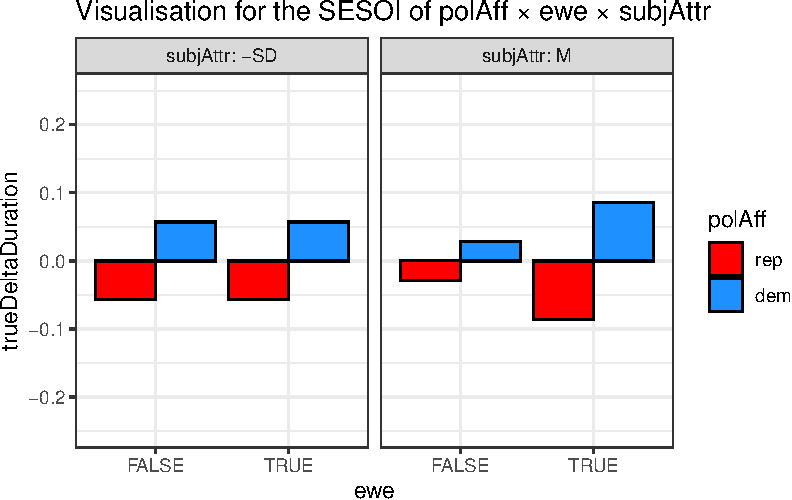
\includegraphics{powerSimulations_files/figure-pdf/fig-trueEffects_3wayInt-1.pdf}

}

\caption{\label{fig-trueEffects_3wayInt}Assumed ΔDuration values for
individuals scoring low (-SD) and average (M) on subjAttr. While
individuals scoring average on subjAttr show a two-way interaction
effect of polAff × ewe of 0.1143, this effect shrinks to zero for
individuals scoring low on subjAttr. These individuals only show the
predicted main effect of polAff (whis is 0.1143).}

\end{figure}%

\subsection{Data Simulation Function}\label{data-simulation-function-2}

We finally define a function that simulates data for the three-way
interaction effect of political affiliation with extreme weather
exposure and attribution of extreme weather events to climate change on
ΔDuration: \texttt{FUN\_sim\_3wayInt}. The function will simulate data
according to the following model, expressed in lme4-lingo:

\texttt{deltaDuration\ \textasciitilde{}\ polAff\ *\ ewe\ *\ subjAttr\ +\ (1\textbar{}subj)\ +\ (1\textbar{}trial)}

The function \texttt{FUN\_sim\_3wayInt} takes, among others, the
following important arguments (in addition to the arguments discussed
for \texttt{FUN\_sim\_2wayInt}):

\begin{itemize}
\item
  \texttt{s\_mean}: \textbf{Sample mean of subjective attribution}.
  Based on results reported by Ogunbode et al. (2019), we set this value
  to 3.67.
\item
  \texttt{s\_sd}: \textbf{Sample SD of subjective attribution}. Based on
  results reported by Ogunbode et al. (2019), we set this value to 0.85.
\item
  \texttt{beta\_s}: \textbf{Fixed main effect of subjective
  attribution}. As we are interested in the moderating role of
  subjective attribution of extreme weather events to climate change, we
  set this main effect to zero.
\item
  \texttt{beta\_p\_s\_inx} \textbf{Fixed two-way interaction effect of
  political affiliation and subjective attribution}. In order to
  accurately model a three-way interaction, one needs to include all
  two-way interactions in statistical models. Therefore, we include this
  two-way interaction, but we assume it to be zero.
\item
  \texttt{beta\_e\_s\_inx} \textbf{Fixed two-way interaction effect of
  extreme weather exposure and subjective attribution}. As before, we
  include this interaction for accurately modelling the three-way
  interaction of interest, but we assume this two-way interaction to be
  zero.
\item
  \texttt{beta\_p\_e\_s\_inx} \textbf{Fixed three-way interaction effect
  of political affiliation, extreme weather exposure, and subjective
  attribution}. We set this initial value to the SESOI derived above,
  i.e.~0.1345. We investigate how changing this effect size impacts
  statistical power, as we are conducting effect-size sensitivity
  analyses for interaction effects.
\end{itemize}

The function is defined below:

\begin{Shaded}
\begin{Highlighting}[]
\CommentTok{\# define data simulation function}
\NormalTok{FUN\_sim\_3wayInt }\OtherTok{\textless{}{-}} \ControlFlowTok{function}\NormalTok{(}
  \AttributeTok{n\_subj         =}                \DecValTok{1000}\NormalTok{, }\CommentTok{\# number of subjects}
  \AttributeTok{n\_subj\_prop\_p  =}           \FunctionTok{c}\NormalTok{(.}\DecValTok{5}\NormalTok{, .}\DecValTok{5}\NormalTok{), }\CommentTok{\# proportion of republican and democrat subjects}
  \AttributeTok{n\_subj\_prop\_e  =}           \FunctionTok{c}\NormalTok{(.}\DecValTok{5}\NormalTok{, .}\DecValTok{5}\NormalTok{), }\CommentTok{\# proportion of subjects without and with extreme weather exposure}
  \AttributeTok{n\_subj\_prop\_s  =}           \FunctionTok{c}\NormalTok{(.}\DecValTok{5}\NormalTok{, .}\DecValTok{5}\NormalTok{), }\CommentTok{\# proportion of subjects with low and high subjective attribution of EWE to CC}
  \AttributeTok{n\_trial        =}                  \DecValTok{25}\NormalTok{, }\CommentTok{\# number of trials}
  \AttributeTok{s\_mean         =}                \FloatTok{3.67}\NormalTok{, }\CommentTok{\# mean of subjAttr, see Ogunbode et al. (2019)}
  \AttributeTok{s\_sd           =}                \FloatTok{0.85}\NormalTok{, }\CommentTok{\# sd of subjAttr, see Ogunbode et al. (2019)}
  \AttributeTok{beta\_0         =}                   \DecValTok{0}\NormalTok{, }\CommentTok{\# intercept (grand mean) for deltaDuration}
  \AttributeTok{beta\_p         =}             \FloatTok{0.4}\SpecialCharTok{/}\FloatTok{3.5}\NormalTok{, }\CommentTok{\# main effect of political affiliation (polAff)}
  \AttributeTok{beta\_e         =}                   \DecValTok{0}\NormalTok{, }\CommentTok{\# main effect of extreme weather exposure (ewe)}
  \AttributeTok{beta\_s         =}                   \DecValTok{0}\NormalTok{, }\CommentTok{\# main effect of subjective attribution of ewe to climate change (subjAttr)}
  \AttributeTok{beta\_p\_e\_inx   =}             \FloatTok{0.4}\SpecialCharTok{/}\FloatTok{3.5}\NormalTok{, }\CommentTok{\# two{-}way interaction effect of polAff and ewe}
  \AttributeTok{beta\_p\_s\_inx   =}                   \DecValTok{0}\NormalTok{, }\CommentTok{\# two{-}way interaction effect of polAff and subjAttr}
  \AttributeTok{beta\_e\_s\_inx   =}                   \DecValTok{0}\NormalTok{, }\CommentTok{\# two{-}way interaction effect of ewe and subjAttr}
  \AttributeTok{beta\_p\_e\_s\_inx =}\NormalTok{      (}\FloatTok{0.4}\SpecialCharTok{/}\FloatTok{3.5}\NormalTok{)}\SpecialCharTok{/}\FloatTok{0.85}\NormalTok{, }\CommentTok{\# three{-}way interaction effect of polAff, ewe, and subjAttr}
  \AttributeTok{subj\_0         =}\NormalTok{                 .}\DecValTok{29}\NormalTok{, }\CommentTok{\# by{-}subject random intercept sd for dt carbon}
  \AttributeTok{trial\_0        =}\NormalTok{                 .}\DecValTok{04}\NormalTok{, }\CommentTok{\# by{-}trial random intercept sd}
  \AttributeTok{sigma          =}         \DecValTok{1}\SpecialCharTok{*}\NormalTok{(.}\DecValTok{29}\FloatTok{+.04}\NormalTok{), }\CommentTok{\# residual (error) sd}
  
  \AttributeTok{truncNums      =}                \ConstantTok{TRUE}\NormalTok{, }\CommentTok{\# should impossible numbers be truncuated?}
  \AttributeTok{setSeed        =}                \ConstantTok{NULL}  \CommentTok{\# seed number to achieve reproducible results. Set to NULL for simulations!}
\NormalTok{) \{}
  
  \CommentTok{\# set seed to achieve reproducible results for demonstration purposes}
  \FunctionTok{set.seed}\NormalTok{(setSeed)}
  
  \CommentTok{\# simulate data for dwell time on carbon information}
\NormalTok{  dataSim }\OtherTok{\textless{}{-}} 
    \CommentTok{\# add random factor subject}
    \FunctionTok{add\_random}\NormalTok{(}\AttributeTok{subj =}\NormalTok{ n\_subj) }\SpecialCharTok{\%\textgreater{}\%} 
    \CommentTok{\# add random factor trial}
    \FunctionTok{add\_random}\NormalTok{(}\AttributeTok{trial =}\NormalTok{ n\_trial) }\SpecialCharTok{\%\textgreater{}\%} 
    \CommentTok{\# add between{-}subject factor political affiliation (with anova contrast)}
    \FunctionTok{add\_between}\NormalTok{(}\StringTok{"subj"}\NormalTok{, }\AttributeTok{polAff =} \FunctionTok{c}\NormalTok{(}\StringTok{"rep"}\NormalTok{, }\StringTok{"dem"}\NormalTok{), }\AttributeTok{.prob =}\NormalTok{ n\_subj\_prop\_p}\SpecialCharTok{*}\NormalTok{n\_subj, }\AttributeTok{.shuffle =} \ConstantTok{TRUE}\NormalTok{) }\SpecialCharTok{\%\textgreater{}\%} 
    \FunctionTok{add\_contrast}\NormalTok{(}\StringTok{"polAff"}\NormalTok{, }\AttributeTok{colnames =} \StringTok{"X\_p"}\NormalTok{, }\AttributeTok{contrast =} \StringTok{"anova"}\NormalTok{) }\SpecialCharTok{\%\textgreater{}\%} 
    \CommentTok{\# add between{-}subject factor extreme weather exposure (with anova contrast)}
    \FunctionTok{add\_between}\NormalTok{(}\StringTok{"subj"}\NormalTok{, }\AttributeTok{ewe =} \FunctionTok{c}\NormalTok{(}\ConstantTok{FALSE}\NormalTok{, }\ConstantTok{TRUE}\NormalTok{), }\AttributeTok{.prob =}\NormalTok{ n\_subj\_prop\_e}\SpecialCharTok{*}\NormalTok{n\_subj, }\AttributeTok{.shuffle =} \ConstantTok{TRUE}\NormalTok{) }\SpecialCharTok{\%\textgreater{}\%} 
    \FunctionTok{add\_contrast}\NormalTok{(}\StringTok{"ewe"}\NormalTok{, }\AttributeTok{colnames =} \StringTok{"X\_e"}\NormalTok{, }\AttributeTok{contrast =} \StringTok{"anova"}\NormalTok{) }\SpecialCharTok{\%\textgreater{}\%} 
    \CommentTok{\# add between{-}subject variable subjective attribution of EWE to climate change}
    \FunctionTok{mutate}\NormalTok{(}
      \AttributeTok{subjAttr =} \FunctionTok{rep}\NormalTok{(}\FunctionTok{rnorm}\NormalTok{(}\AttributeTok{n =}\NormalTok{ n\_subj, }\AttributeTok{mean =}\NormalTok{ s\_mean, }\AttributeTok{sd =}\NormalTok{ s\_sd), }\AttributeTok{each =}\NormalTok{ n\_trial),}
      \AttributeTok{subjAttr\_c =} \FunctionTok{scale}\NormalTok{(subjAttr, }\AttributeTok{center =} \ConstantTok{TRUE}\NormalTok{, }\AttributeTok{scale =} \ConstantTok{FALSE}\NormalTok{)[,}\DecValTok{1}\NormalTok{]}
\NormalTok{    ) }\SpecialCharTok{\%\textgreater{}\%} 
    \CommentTok{\# add by{-}subject random intercept}
    \FunctionTok{add\_ranef}\NormalTok{(}\StringTok{"subj"}\NormalTok{, }\AttributeTok{S\_0 =}\NormalTok{ subj\_0) }\SpecialCharTok{\%\textgreater{}\%} 
    \CommentTok{\# add by{-}trial random intercept}
    \FunctionTok{add\_ranef}\NormalTok{(}\StringTok{"trial"}\NormalTok{, }\AttributeTok{T\_0 =}\NormalTok{ trial\_0) }\SpecialCharTok{\%\textgreater{}\%} 
    \CommentTok{\# add error term}
    \FunctionTok{add\_ranef}\NormalTok{(}\AttributeTok{e\_st =}\NormalTok{ sigma) }\SpecialCharTok{\%\textgreater{}\%} 
    \CommentTok{\# add response values}
    \FunctionTok{mutate}\NormalTok{(}
      \CommentTok{\# add together fixed and random effects for each effect}
      \AttributeTok{B\_0 =}\NormalTok{ beta\_0 }\SpecialCharTok{+}\NormalTok{ S\_0 }\SpecialCharTok{+}\NormalTok{ T\_0,}
      \AttributeTok{B\_p =}\NormalTok{ beta\_p,}
      \AttributeTok{B\_e =}\NormalTok{ beta\_e,}
      \AttributeTok{B\_s =}\NormalTok{ beta\_s,}
      \AttributeTok{B\_p\_e\_inx =}\NormalTok{ beta\_p\_e\_inx,}
      \AttributeTok{B\_p\_s\_inx =}\NormalTok{ beta\_p\_s\_inx,}
      \AttributeTok{B\_e\_s\_inx =}\NormalTok{ beta\_e\_s\_inx,}
      \AttributeTok{B\_p\_e\_s\_inx =}\NormalTok{ beta\_p\_e\_s\_inx,}
      \CommentTok{\# calculate dv by adding each effect term multiplied by the relevant}
      \CommentTok{\# effect{-}coded factors and adding the error term}
      \AttributeTok{deltaDuration =} 
\NormalTok{        B\_0 }\SpecialCharTok{+}\NormalTok{ e\_st }\SpecialCharTok{+}
\NormalTok{        (X\_p }\SpecialCharTok{*}\NormalTok{ B\_p) }\SpecialCharTok{+}
\NormalTok{        (X\_e }\SpecialCharTok{*}\NormalTok{ B\_e) }\SpecialCharTok{+}
\NormalTok{        (subjAttr\_c }\SpecialCharTok{*}\NormalTok{ B\_s) }\SpecialCharTok{+}
\NormalTok{        (X\_p }\SpecialCharTok{*}\NormalTok{ X\_e }\SpecialCharTok{*}\NormalTok{ B\_p\_e\_inx) }\SpecialCharTok{+}
\NormalTok{        (X\_p }\SpecialCharTok{*}\NormalTok{ subjAttr\_c }\SpecialCharTok{*}\NormalTok{ B\_p\_s\_inx) }\SpecialCharTok{+}
\NormalTok{        (X\_e }\SpecialCharTok{*}\NormalTok{ subjAttr\_c }\SpecialCharTok{*}\NormalTok{ B\_e\_s\_inx) }\SpecialCharTok{+}
\NormalTok{        (X\_p }\SpecialCharTok{*}\NormalTok{ X\_e }\SpecialCharTok{*}\NormalTok{ subjAttr\_c }\SpecialCharTok{*}\NormalTok{ B\_p\_e\_s\_inx)}
\NormalTok{    )}
  
  \CommentTok{\# unset seed}
  \FunctionTok{set.seed}\NormalTok{(}\ConstantTok{NULL}\NormalTok{)}
  
  \CommentTok{\# truncuate impossible deltaDurations}
  \ControlFlowTok{if}\NormalTok{(truncNums) \{}
\NormalTok{    dataSim }\OtherTok{\textless{}{-}}\NormalTok{ dataSim }\SpecialCharTok{\%\textgreater{}\%} 
      \FunctionTok{mutate}\NormalTok{(}\AttributeTok{deltaDuration =} \FunctionTok{if\_else}\NormalTok{(deltaDuration }\SpecialCharTok{\textless{}} \SpecialCharTok{{-}}\DecValTok{1}\NormalTok{, }\SpecialCharTok{{-}}\DecValTok{1}\NormalTok{,}
        \FunctionTok{if\_else}\NormalTok{(deltaDuration }\SpecialCharTok{\textgreater{}} \DecValTok{1}\NormalTok{, }\DecValTok{1}\NormalTok{, deltaDuration)))}
\NormalTok{  \}}
  
  \CommentTok{\# run a linear mixed effects model and check summary}
\NormalTok{  mod }\OtherTok{\textless{}{-}} \FunctionTok{lmer}\NormalTok{(}
\NormalTok{    deltaDuration }\SpecialCharTok{\textasciitilde{}}\NormalTok{ polAff}\SpecialCharTok{*}\NormalTok{ewe}\SpecialCharTok{*}\NormalTok{subjAttr\_c }\SpecialCharTok{+}\NormalTok{ (}\DecValTok{1} \SpecialCharTok{|}\NormalTok{ subj) }\SpecialCharTok{+}\NormalTok{ (}\DecValTok{1} \SpecialCharTok{|}\NormalTok{ trial),}
    \AttributeTok{data =}\NormalTok{ dataSim}
\NormalTok{  )}
\NormalTok{  mod.sum }\OtherTok{\textless{}{-}} \FunctionTok{summary}\NormalTok{(mod)}

  \CommentTok{\# get results in tidy format}
\NormalTok{  mod.broom }\OtherTok{\textless{}{-}}\NormalTok{ broom.mixed}\SpecialCharTok{::}\FunctionTok{tidy}\NormalTok{(mod)}

  \FunctionTok{return}\NormalTok{(}\FunctionTok{list}\NormalTok{(}
    \AttributeTok{dataSim =}\NormalTok{ dataSim,}
    \AttributeTok{modelLmer =}\NormalTok{ mod,}
    \AttributeTok{modelResults =}\NormalTok{ mod.broom}
\NormalTok{  ))}
  
\NormalTok{\}}
\end{Highlighting}
\end{Shaded}

We call the function once and extract the results of this single
simulation:

\begin{Shaded}
\begin{Highlighting}[]
\CommentTok{\# Note to myself: Consider setting beta\_p = 0.4/3.5, beta\_p\_e\_inx = 0.4/3.5,}
\CommentTok{\# and beta\_p\_e\_s\_inx to 2 * 0.4/3.5/(2*.85).}
\CommentTok{\# This way, the interaction effect polAff:ewe is 0.4/3.5 for individuals}
\CommentTok{\# with an average subjAttr (subjAttr\_c = 0). For individuals with}
\CommentTok{\# subjAttr = mean {-} SD, polAff:ewe is 0. For individuals with subjAttr = mean + SD,}
\CommentTok{\# polAff:ewe is  2 * 0.4/3.5.}

\NormalTok{out }\OtherTok{\textless{}{-}} \FunctionTok{FUN\_sim\_3wayInt}\NormalTok{(}
  \AttributeTok{n\_subj         =}                \DecValTok{1000}\NormalTok{, }\CommentTok{\# number of subjects}
  \AttributeTok{n\_subj\_prop\_p  =}           \FunctionTok{c}\NormalTok{(.}\DecValTok{5}\NormalTok{, .}\DecValTok{5}\NormalTok{), }\CommentTok{\# proportion of republican and democrat subjects}
  \AttributeTok{n\_subj\_prop\_e  =}           \FunctionTok{c}\NormalTok{(.}\DecValTok{5}\NormalTok{, .}\DecValTok{5}\NormalTok{), }\CommentTok{\# proportion of subjects without and with extreme weather exposure}
  \AttributeTok{n\_subj\_prop\_s  =}           \FunctionTok{c}\NormalTok{(.}\DecValTok{5}\NormalTok{, .}\DecValTok{5}\NormalTok{), }\CommentTok{\# proportion of subjects with low and high subjective attribution of EWE to CC}
  \AttributeTok{n\_trial        =}                  \DecValTok{25}\NormalTok{, }\CommentTok{\# number of trials}
  \AttributeTok{s\_mean         =}                \FloatTok{3.67}\NormalTok{, }\CommentTok{\# mean of subjAttr, see Ogunbode et al. (2019)}
  \AttributeTok{s\_sd           =}                \FloatTok{0.85}\NormalTok{, }\CommentTok{\# sd of subjAttr, see Ogunbode et al. (2019)}
  \AttributeTok{beta\_0         =}                   \DecValTok{0}\NormalTok{, }\CommentTok{\# intercept (grand mean) for deltaDuration}
  \AttributeTok{beta\_p         =}             \FloatTok{0.4}\SpecialCharTok{/}\FloatTok{3.5}\NormalTok{, }\CommentTok{\# main effect of political affiliation (polAff)}
  \AttributeTok{beta\_e         =}                   \DecValTok{0}\NormalTok{, }\CommentTok{\# main effect of extreme weather exposure (ewe)}
  \AttributeTok{beta\_s         =}                   \DecValTok{0}\NormalTok{, }\CommentTok{\# main effect of subjective attribution of ewe to climate change (subjAttr)}
  \AttributeTok{beta\_p\_e\_inx   =}             \FloatTok{0.4}\SpecialCharTok{/}\FloatTok{3.5}\NormalTok{, }\CommentTok{\# two{-}way interaction effect of polAff and ewe}
  \AttributeTok{beta\_p\_s\_inx   =}                   \DecValTok{0}\NormalTok{, }\CommentTok{\# two{-}way interaction effect of polAff and subjAttr}
  \AttributeTok{beta\_e\_s\_inx   =}                   \DecValTok{0}\NormalTok{, }\CommentTok{\# two{-}way interaction effect of ewe and subjAttr}
  \AttributeTok{beta\_p\_e\_s\_inx =}\NormalTok{      (}\FloatTok{0.4}\SpecialCharTok{/}\FloatTok{3.5}\NormalTok{)}\SpecialCharTok{/}\FloatTok{0.85}\NormalTok{, }\CommentTok{\# three{-}way interaction effect of polAff, ewe, and subjAttr}
  \AttributeTok{subj\_0         =}\NormalTok{                 .}\DecValTok{29}\NormalTok{, }\CommentTok{\# by{-}subject random intercept sd for dt carbon}
  \AttributeTok{trial\_0        =}\NormalTok{                 .}\DecValTok{04}\NormalTok{, }\CommentTok{\# by{-}trial random intercept sd}
  \AttributeTok{sigma          =}         \DecValTok{1}\SpecialCharTok{*}\NormalTok{(.}\DecValTok{29}\FloatTok{+.04}\NormalTok{), }\CommentTok{\# residual (error) sd}
  
  \AttributeTok{truncNums      =}                \ConstantTok{TRUE}\NormalTok{, }\CommentTok{\# should impossible numbers be truncuated?}
  \AttributeTok{setSeed        =}                 \DecValTok{123}  \CommentTok{\# seed number to achieve reproducible results. Set to NULL for simulations!}
\NormalTok{)}

\CommentTok{\# Get results table}
\NormalTok{resultsTable }\OtherTok{\textless{}{-}}\NormalTok{ out}\SpecialCharTok{$}\NormalTok{modelResults }\SpecialCharTok{\%\textgreater{}\%} 
  \FunctionTok{select}\NormalTok{(}\SpecialCharTok{{-}}\FunctionTok{c}\NormalTok{(std.error, statistic, df)) }\SpecialCharTok{\%\textgreater{}\%} 
  \FunctionTok{mutate}\NormalTok{(}\FunctionTok{across}\NormalTok{(}\FunctionTok{where}\NormalTok{(is\_double), }\SpecialCharTok{\textasciitilde{}} \FunctionTok{round}\NormalTok{(.x, }\DecValTok{4}\NormalTok{))) }\SpecialCharTok{\%\textgreater{}\%} 
\NormalTok{  knitr}\SpecialCharTok{::}\FunctionTok{kable}\NormalTok{()}
\NormalTok{formulaUsedForFit }\OtherTok{\textless{}{-}} \FunctionTok{paste}\NormalTok{(}\FunctionTok{as.character}\NormalTok{(}\FunctionTok{formula}\NormalTok{(out}\SpecialCharTok{$}\NormalTok{modelLmer))[}\FunctionTok{c}\NormalTok{(}\DecValTok{2}\NormalTok{,}\DecValTok{1}\NormalTok{,}\DecValTok{3}\NormalTok{)], }\AttributeTok{collapse =} \StringTok{" "}\NormalTok{)}

\CommentTok{\# Create predictions plot}

\CommentTok{\# refit model to dispaly subjAttr levels in original metric (not mean centered)}
\NormalTok{m }\OtherTok{\textless{}{-}} \FunctionTok{lmer}\NormalTok{(}
\NormalTok{  deltaDuration }\SpecialCharTok{\textasciitilde{}}\NormalTok{ polAff}\SpecialCharTok{*}\NormalTok{ewe}\SpecialCharTok{*}\NormalTok{subjAttr }\SpecialCharTok{+}\NormalTok{ (}\DecValTok{1} \SpecialCharTok{|}\NormalTok{ subj) }\SpecialCharTok{+}\NormalTok{ (}\DecValTok{1} \SpecialCharTok{|}\NormalTok{ trial),}
  \AttributeTok{data =}\NormalTok{ out}\SpecialCharTok{$}\NormalTok{dataSim}
\NormalTok{)}
\CommentTok{\# define spotlights for spotlight analysis}
\NormalTok{spotlights }\OtherTok{\textless{}{-}} \FunctionTok{c}\NormalTok{(}\FloatTok{3.67} \SpecialCharTok{{-}} \FloatTok{0.85}\NormalTok{, }\FloatTok{3.67}\NormalTok{, }\FloatTok{3.67} \SpecialCharTok{+} \FloatTok{0.85}\NormalTok{)}

\CommentTok{\# create plot showing predictions}
\NormalTok{p.demo}\FloatTok{.3}\NormalTok{wayInt.pred }\OtherTok{\textless{}{-}} \FunctionTok{predict\_response}\NormalTok{(m, }\AttributeTok{terms =} \FunctionTok{c}\NormalTok{(}\StringTok{"ewe"}\NormalTok{, }\StringTok{"polAff"}\NormalTok{, }\StringTok{"subjAttr[spotlights]"}\NormalTok{))}
\NormalTok{p.demo}\FloatTok{.3}\NormalTok{wayInt }\OtherTok{\textless{}{-}}\NormalTok{ p.demo}\FloatTok{.3}\NormalTok{wayInt.pred }\SpecialCharTok{\%\textgreater{}\%} 
  \FunctionTok{plot}\NormalTok{(}\AttributeTok{colors =} \FunctionTok{c}\NormalTok{(}\StringTok{"red"}\NormalTok{, }\StringTok{"dodgerblue"}\NormalTok{)) }\SpecialCharTok{+}
  \FunctionTok{coord\_cartesian}\NormalTok{(}\AttributeTok{ylim =} \FunctionTok{c}\NormalTok{(}\SpecialCharTok{{-}}\NormalTok{.}\DecValTok{25}\NormalTok{, .}\DecValTok{25}\NormalTok{)) }\SpecialCharTok{+}
  \FunctionTok{theme\_bw}\NormalTok{()}
\end{Highlighting}
\end{Shaded}

Figure~\ref{fig-demoFUNSim_3wayInt} visualizes predictions based on this
single simulation and Table~\ref{tbl-demoFUNSim_3wayInt} summarizes the
statistical results of fitting the actual model used in data generation
to the simulated data.

\begin{figure}

\centering{

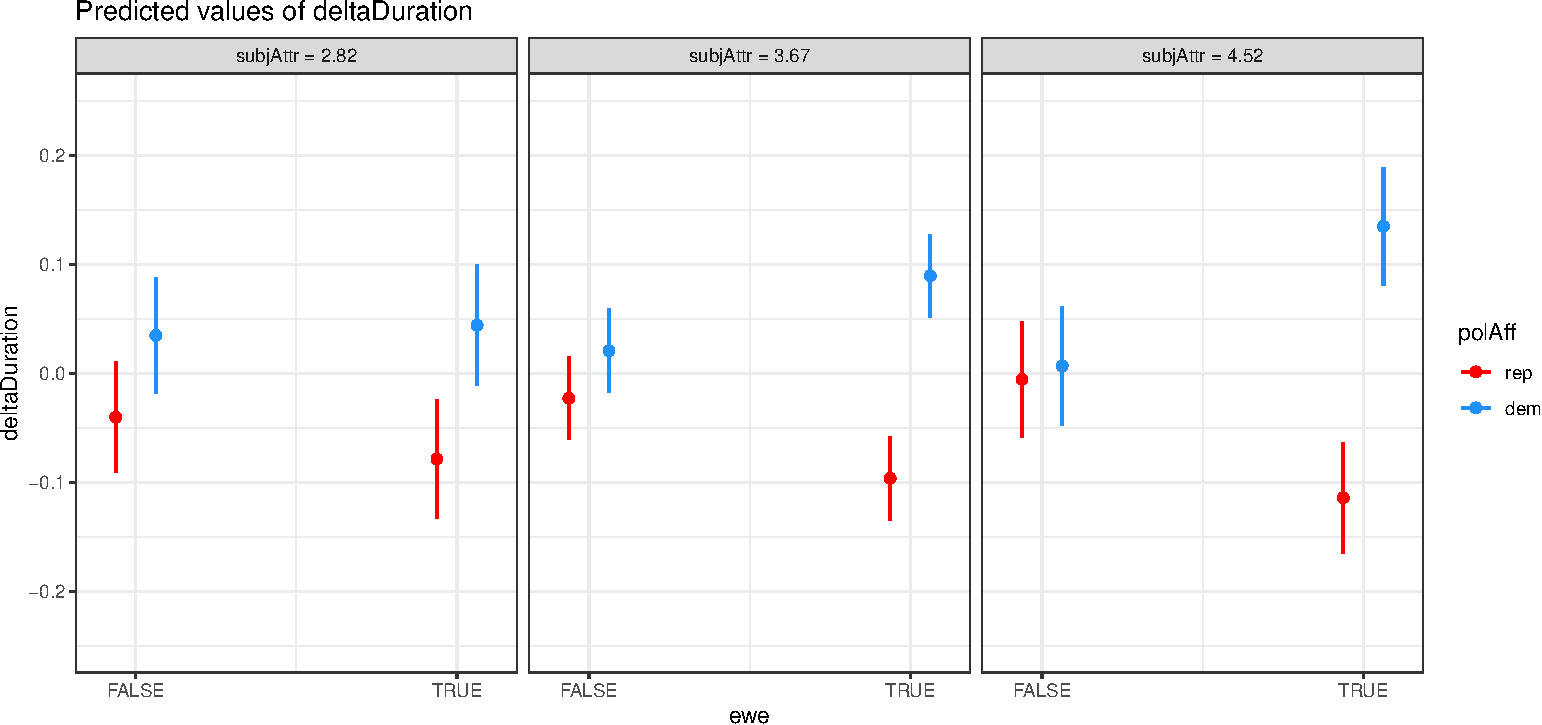
\includegraphics{powerSimulations_files/figure-pdf/fig-demoFUNSim_3wayInt-1.pdf}

}

\caption{\label{fig-demoFUNSim_3wayInt}Visual representation of results
of one simulation created using \texttt{FUN\_sim\_3wayInt}. Points
indicate the predicted means surrounded by 95\% Confidence Intervals.
Panels indicate predictions for different values of subjAttr (Mean - SD,
Mean, and Mean + SD).}

\end{figure}%

\phantomsection\label{tbl-demoFUNSim_3wayInt}
\begin{longtable}[]{@{}
  >{\raggedright\arraybackslash}p{(\columnwidth - 8\tabcolsep) * \real{0.1184}}
  >{\raggedright\arraybackslash}p{(\columnwidth - 8\tabcolsep) * \real{0.1184}}
  >{\raggedright\arraybackslash}p{(\columnwidth - 8\tabcolsep) * \real{0.5395}}
  >{\raggedleft\arraybackslash}p{(\columnwidth - 8\tabcolsep) * \real{0.1184}}
  >{\raggedleft\arraybackslash}p{(\columnwidth - 8\tabcolsep) * \real{0.1053}}@{}}

\caption{\label{tbl-demoFUNSim_3wayInt}Statistical results of one
simulation created using \texttt{FUN\_sim\_3wayInt}. Data was fit using
deltaDuration \textasciitilde{} polAff * ewe * subjAttr\_c + (1
\textbar{} subj) + (1 \textbar{} trial). Note that subjAttr is mean
centered to ease interpretation of lower-level interactions and main
effects.}

\tabularnewline

\toprule\noalign{}
\begin{minipage}[b]{\linewidth}\raggedright
effect
\end{minipage} & \begin{minipage}[b]{\linewidth}\raggedright
group
\end{minipage} & \begin{minipage}[b]{\linewidth}\raggedright
term
\end{minipage} & \begin{minipage}[b]{\linewidth}\raggedleft
estimate
\end{minipage} & \begin{minipage}[b]{\linewidth}\raggedleft
p.value
\end{minipage} \\
\midrule\noalign{}
\endhead
\bottomrule\noalign{}
\endlastfoot
fixed & NA & (Intercept) & -0.0022 & 0.8478 \\
fixed & NA & polAff.dem-rep & 0.1149 & 0.0000 \\
fixed & NA & ewe.TRUE-FALSE & -0.0023 & 0.9031 \\
fixed & NA & subjAttr\_c & 0.0091 & 0.4141 \\
fixed & NA & polAff.dem-rep:ewe.TRUE-FALSE & 0.1426 & 0.0001 \\
fixed & NA & polAff.dem-rep:subjAttr\_c & 0.0187 & 0.4025 \\
fixed & NA & ewe.TRUE-FALSE:subjAttr\_c & 0.0142 & 0.5239 \\
fixed & NA & polAff.dem-rep:ewe.TRUE-FALSE:subjAttr\_c & 0.1111 &
0.0130 \\
ran\_pars & subj & sd\_\_(Intercept) & 0.2849 & NA \\
ran\_pars & trial & sd\_\_(Intercept) & 0.0323 & NA \\
ran\_pars & Residual & sd\_\_Observation & 0.3240 & NA \\

\end{longtable}

\subsection{Power Simulation}\label{power-simulation-2}

In the following code, the simulations are calculated. We do not
recommend executing this code junk as it takes several hours to run.

\begin{Shaded}
\begin{Highlighting}[]
\NormalTok{FUN\_sim\_3wayInt\_pwr }\OtherTok{\textless{}{-}} \ControlFlowTok{function}\NormalTok{(sim, ...)\{}
\NormalTok{  out }\OtherTok{\textless{}{-}} \FunctionTok{FUN\_sim\_3wayInt}\NormalTok{(...)}
\NormalTok{  modelResults }\OtherTok{\textless{}{-}}\NormalTok{ out}\SpecialCharTok{$}\NormalTok{modelResults }\SpecialCharTok{\%\textgreater{}\%} 
    \FunctionTok{mutate}\NormalTok{(}\AttributeTok{sim =}\NormalTok{ sim) }\SpecialCharTok{\%\textgreater{}\%} 
    \FunctionTok{relocate}\NormalTok{(sim)}
  \FunctionTok{return}\NormalTok{(modelResults)}
\NormalTok{\}}

\CommentTok{\# How many simulations should be run?}
\NormalTok{n\_sims }\OtherTok{\textless{}{-}} \DecValTok{1000}

\CommentTok{\# What are the breaks for number of subjects we would like to calculate power for?}
\NormalTok{breaks\_subj }\OtherTok{\textless{}{-}} \FunctionTok{c}\NormalTok{(}\DecValTok{900}\NormalTok{, }\DecValTok{950}\NormalTok{, }\DecValTok{1000}\NormalTok{)}

\CommentTok{\# What are the breaks for SESOI?}
\NormalTok{breaks\_sesoi }\OtherTok{\textless{}{-}}\NormalTok{ (}\FloatTok{0.4}\SpecialCharTok{/}\FloatTok{3.5}\NormalTok{)}\SpecialCharTok{/}\FloatTok{0.85} \SpecialCharTok{*} \FunctionTok{seq}\NormalTok{(}\DecValTok{1}\NormalTok{, }\DecValTok{2}\NormalTok{, .}\DecValTok{25}\NormalTok{)}

\CommentTok{\# What are the breaks for different error SDs?}
\NormalTok{breaks\_sigma }\OtherTok{\textless{}{-}} \FunctionTok{c}\NormalTok{((.}\DecValTok{29}\FloatTok{+.04}\NormalTok{), }\DecValTok{2}\SpecialCharTok{*}\NormalTok{(.}\DecValTok{29}\FloatTok{+.04}\NormalTok{))}

\NormalTok{res\_3wayInt }\OtherTok{\textless{}{-}} \FunctionTok{tibble}\NormalTok{()}
\ControlFlowTok{for}\NormalTok{ (s }\ControlFlowTok{in} \FunctionTok{seq\_along}\NormalTok{(breaks\_sigma)) \{}
  
\NormalTok{  res\_sesoi }\OtherTok{\textless{}{-}} \FunctionTok{tibble}\NormalTok{()}
  \ControlFlowTok{for}\NormalTok{ (sesoi }\ControlFlowTok{in} \FunctionTok{seq\_along}\NormalTok{(breaks\_sesoi)) \{}
    
\NormalTok{    res\_nSubj }\OtherTok{\textless{}{-}} \FunctionTok{tibble}\NormalTok{()}
    \ControlFlowTok{for}\NormalTok{ (nSubj }\ControlFlowTok{in} \FunctionTok{seq\_along}\NormalTok{(breaks\_subj)) \{}
      
      \CommentTok{\# Give feedback regarding which model is simulated}
      \FunctionTok{cat}\NormalTok{(}\FunctionTok{paste0}\NormalTok{(}
        \StringTok{"Simulation:}\SpecialCharTok{\textbackslash{}n}\StringTok{"}\NormalTok{,}
        \StringTok{"  sigma = "}\NormalTok{, }\FunctionTok{round}\NormalTok{(breaks\_sigma[s], }\DecValTok{4}\NormalTok{), }\StringTok{"}\SpecialCharTok{\textbackslash{}n}\StringTok{"}\NormalTok{,}
        \StringTok{"  sesoi = "}\NormalTok{, }\FunctionTok{round}\NormalTok{(breaks\_sesoi[sesoi], }\DecValTok{4}\NormalTok{), }\StringTok{"}\SpecialCharTok{\textbackslash{}n}\StringTok{"}\NormalTok{,}
        \StringTok{"  nSubject = "}\NormalTok{, breaks\_subj[nSubj], }\StringTok{"}\SpecialCharTok{\textbackslash{}n}\StringTok{"}
\NormalTok{      ))}
      
      \CommentTok{\# Start timer}
      \FunctionTok{cat}\NormalTok{(}\FunctionTok{paste0}\NormalTok{(}\StringTok{"Start date time: "}\NormalTok{, lubridate}\SpecialCharTok{::}\FunctionTok{now}\NormalTok{(), }\StringTok{"}\SpecialCharTok{\textbackslash{}n}\StringTok{"}\NormalTok{))}
      \FunctionTok{tic}\NormalTok{()}
      
      \CommentTok{\# Loop over simulations}
\NormalTok{      pwr }\OtherTok{\textless{}{-}} \FunctionTok{map\_df}\NormalTok{(}
        \DecValTok{1}\SpecialCharTok{:}\NormalTok{n\_sims, }
\NormalTok{        FUN\_sim\_3wayInt\_pwr,}
        \AttributeTok{n\_subj =}\NormalTok{ breaks\_subj[nSubj],}
        \AttributeTok{beta\_p\_e\_s\_inx =}\NormalTok{ breaks\_sesoi[sesoi],}
        \AttributeTok{sigma =}\NormalTok{ breaks\_sigma[s]}
\NormalTok{      )}
      
      \CommentTok{\# Stop timer and calculate elapsed time}
\NormalTok{      elapsed\_time }\OtherTok{\textless{}{-}} \FunctionTok{toc}\NormalTok{(}\AttributeTok{quiet =} \ConstantTok{TRUE}\NormalTok{)}
\NormalTok{      elapsed\_seconds }\OtherTok{\textless{}{-}}\NormalTok{ elapsed\_time}\SpecialCharTok{$}\NormalTok{toc }\SpecialCharTok{{-}}\NormalTok{ elapsed\_time}\SpecialCharTok{$}\NormalTok{tic}
\NormalTok{      elapsed\_minutes }\OtherTok{\textless{}{-}}\NormalTok{ elapsed\_seconds }\SpecialCharTok{/} \DecValTok{60}
      \FunctionTok{cat}\NormalTok{(}\FunctionTok{paste0}\NormalTok{(}\StringTok{"End date time: "}\NormalTok{, lubridate}\SpecialCharTok{::}\FunctionTok{now}\NormalTok{(), }\StringTok{"}\SpecialCharTok{\textbackslash{}n}\StringTok{"}\NormalTok{))}
      \FunctionTok{cat}\NormalTok{(}\StringTok{"Elapsed time: "}\NormalTok{, elapsed\_minutes, }\StringTok{" minutes}\SpecialCharTok{\textbackslash{}n\textbackslash{}n}\StringTok{"}\NormalTok{)}
      
      \CommentTok{\# Add number of subjects to pwr}
\NormalTok{      pwr }\OtherTok{\textless{}{-}}\NormalTok{ pwr }\SpecialCharTok{\%\textgreater{}\%} 
        \FunctionTok{mutate}\NormalTok{(}
          \AttributeTok{nSubjects =}\NormalTok{ breaks\_subj[nSubj],}
          \AttributeTok{sesoi =}\NormalTok{ breaks\_sesoi[sesoi],}
          \AttributeTok{sigma =}\NormalTok{ breaks\_sigma[s]}
\NormalTok{        )}
      
      \CommentTok{\# Add results to the results table}
\NormalTok{      res\_nSubj }\OtherTok{\textless{}{-}}\NormalTok{ res\_nSubj }\SpecialCharTok{\%\textgreater{}\%}
        \FunctionTok{rbind}\NormalTok{(pwr)}
\NormalTok{    \}}
    
    \CommentTok{\# Add results to the results table}
\NormalTok{    res\_sesoi }\OtherTok{\textless{}{-}}\NormalTok{ res\_sesoi }\SpecialCharTok{\%\textgreater{}\%} 
      \FunctionTok{rbind}\NormalTok{(res\_nSubj)}
\NormalTok{  \}}
  
  \CommentTok{\# Add results to the results table}
\NormalTok{  res\_3wayInt }\OtherTok{\textless{}{-}}\NormalTok{ res\_3wayInt }\SpecialCharTok{\%\textgreater{}\%} 
    \FunctionTok{rbind}\NormalTok{(res\_sesoi)}
  
\NormalTok{\}}

\NormalTok{res\_3wayInt.summary }\OtherTok{\textless{}{-}}\NormalTok{ res\_3wayInt }\SpecialCharTok{\%\textgreater{}\%} 
  \FunctionTok{filter}\NormalTok{(term }\SpecialCharTok{==} \StringTok{"polAff.dem{-}rep:ewe.TRUE{-}FALSE:subjAttr\_c"}\NormalTok{) }\SpecialCharTok{\%\textgreater{}\%} 
  \FunctionTok{group\_by}\NormalTok{(sigma, sesoi, nSubjects) }\SpecialCharTok{\%\textgreater{}\%} 
  \FunctionTok{summarise}\NormalTok{(}
    \AttributeTok{power =} \FunctionTok{mean}\NormalTok{(p.value }\SpecialCharTok{\textless{}} \FloatTok{0.05}\NormalTok{),}
    \AttributeTok{ci.lower =} \FunctionTok{binom.confint}\NormalTok{(power}\SpecialCharTok{*}\NormalTok{n\_sims, n\_sims, }\AttributeTok{methods =} \StringTok{"exact"}\NormalTok{)}\SpecialCharTok{$}\NormalTok{lower,}
    \AttributeTok{ci.upper =} \FunctionTok{binom.confint}\NormalTok{(power}\SpecialCharTok{*}\NormalTok{n\_sims, n\_sims, }\AttributeTok{methods =} \StringTok{"exact"}\NormalTok{)}\SpecialCharTok{$}\NormalTok{upper,}
    \AttributeTok{.groups =} \StringTok{\textquotesingle{}drop\textquotesingle{}}
\NormalTok{  ) }\SpecialCharTok{\%\textgreater{}\%} 
  \FunctionTok{mutate}\NormalTok{(}
    \AttributeTok{sigma\_fact =} \FunctionTok{factor}\NormalTok{(}\FunctionTok{format}\NormalTok{(}\FunctionTok{round}\NormalTok{(sigma, }\DecValTok{4}\NormalTok{), }\AttributeTok{nsmall =} \DecValTok{4}\NormalTok{)),}
    \AttributeTok{sigma\_level =} \FunctionTok{match}\NormalTok{(sigma\_fact, }\FunctionTok{levels}\NormalTok{(sigma\_fact)),}
    \AttributeTok{sesoi\_fact =} \FunctionTok{factor}\NormalTok{(}\FunctionTok{format}\NormalTok{(}\FunctionTok{round}\NormalTok{(sesoi, }\DecValTok{4}\NormalTok{), }\AttributeTok{nsmall =} \DecValTok{4}\NormalTok{)),}
    \AttributeTok{sesoi\_level =} \FunctionTok{match}\NormalTok{(sesoi\_fact, }\FunctionTok{levels}\NormalTok{(sesoi\_fact))}
\NormalTok{  )}

\CommentTok{\# Save results in a list object}
\NormalTok{time }\OtherTok{\textless{}{-}} \FunctionTok{format}\NormalTok{(}\FunctionTok{Sys.time}\NormalTok{(), }\StringTok{"\%Y\%m\%d\_\%H\%M"}\NormalTok{)}
\NormalTok{fileName }\OtherTok{\textless{}{-}} \FunctionTok{paste0}\NormalTok{(}\StringTok{"res\_3wayInt"}\NormalTok{, }\StringTok{"\_"}\NormalTok{, time, }\StringTok{".RDS"}\NormalTok{)}
\FunctionTok{saveRDS}\NormalTok{(}
  \FunctionTok{list}\NormalTok{(}
    \AttributeTok{res\_3wayInt =}\NormalTok{ res\_3wayInt,}
    \AttributeTok{res\_3wayInt.summary =}\NormalTok{ res\_3wayInt.summary}
\NormalTok{  ),}
  \AttributeTok{file =} \FunctionTok{file.path}\NormalTok{(}\StringTok{"../powerSimulationsOutput"}\NormalTok{, fileName)}
\NormalTok{)}
\end{Highlighting}
\end{Shaded}

We retrieve pre-run results:

\begin{Shaded}
\begin{Highlighting}[]
\CommentTok{\# Load power simulation data}
\NormalTok{resList\_3wayInt }\OtherTok{\textless{}{-}} \FunctionTok{readRDS}\NormalTok{(}\FunctionTok{file.path}\NormalTok{(}\StringTok{"../powerSimulationsOutput"}\NormalTok{, }\StringTok{"res\_3wayInt\_20240814\_1612.RDS"}\NormalTok{)) }
\NormalTok{resList\_3wayInt.summary }\OtherTok{\textless{}{-}}\NormalTok{ resList\_3wayInt}\SpecialCharTok{$}\NormalTok{res\_3wayInt.summary}

\CommentTok{\# Extract power values for some specific effect sizes at N = 1000}
\NormalTok{powerValues }\OtherTok{\textless{}{-}}\NormalTok{ resList\_3wayInt.summary }\SpecialCharTok{\%\textgreater{}\%} 
  \FunctionTok{filter}\NormalTok{(sigma\_fact }\SpecialCharTok{==} \StringTok{"0.3300"}\NormalTok{) }\SpecialCharTok{\%\textgreater{}\%} 
  \FunctionTok{filter}\NormalTok{(sesoi\_fact }\SpecialCharTok{==} \StringTok{"0.1345"}\NormalTok{) }\SpecialCharTok{\%\textgreater{}\%} 
  \FunctionTok{filter}\NormalTok{(nSubjects }\SpecialCharTok{==} \DecValTok{950}\NormalTok{) }\SpecialCharTok{\%\textgreater{}\%} 
  \FunctionTok{mutate}\NormalTok{(}\AttributeTok{power\_str =} \FunctionTok{paste0}\NormalTok{(}\FunctionTok{round}\NormalTok{(power}\SpecialCharTok{*}\DecValTok{100}\NormalTok{, }\DecValTok{2}\NormalTok{), }\StringTok{"\%"}\NormalTok{)) }\SpecialCharTok{\%\textgreater{}\%} 
  \FunctionTok{pull}\NormalTok{(power\_str)}

\CommentTok{\# Extract number of simulations}
\NormalTok{label\_nSimulations }\OtherTok{\textless{}{-}}\NormalTok{ resList\_3wayInt}\SpecialCharTok{$}\NormalTok{res\_3wayInt}\SpecialCharTok{$}\NormalTok{sim }\SpecialCharTok{\%\textgreater{}\%} \FunctionTok{n\_distinct}\NormalTok{()}

\CommentTok{\# Repeat breaks\_sesoi}
\NormalTok{breaks\_sesoi }\OtherTok{\textless{}{-}}\NormalTok{ (}\FloatTok{0.4}\SpecialCharTok{/}\FloatTok{3.5}\NormalTok{)}\SpecialCharTok{/}\NormalTok{(}\FloatTok{0.85}\NormalTok{) }\SpecialCharTok{*} \FunctionTok{seq}\NormalTok{(}\DecValTok{1}\NormalTok{, }\DecValTok{2}\NormalTok{, .}\DecValTok{25}\NormalTok{)}
\end{Highlighting}
\end{Shaded}

Figure~\ref{fig-checkSims-threeWayInt} displays the distribution of
estimated fixed effects across all simulations. The figure shows that
the estimated fixed effects are close to the true ones provided as input
in the data simulation function, validating that simulations worked as
expected.

\begin{figure}

\centering{

\centering{

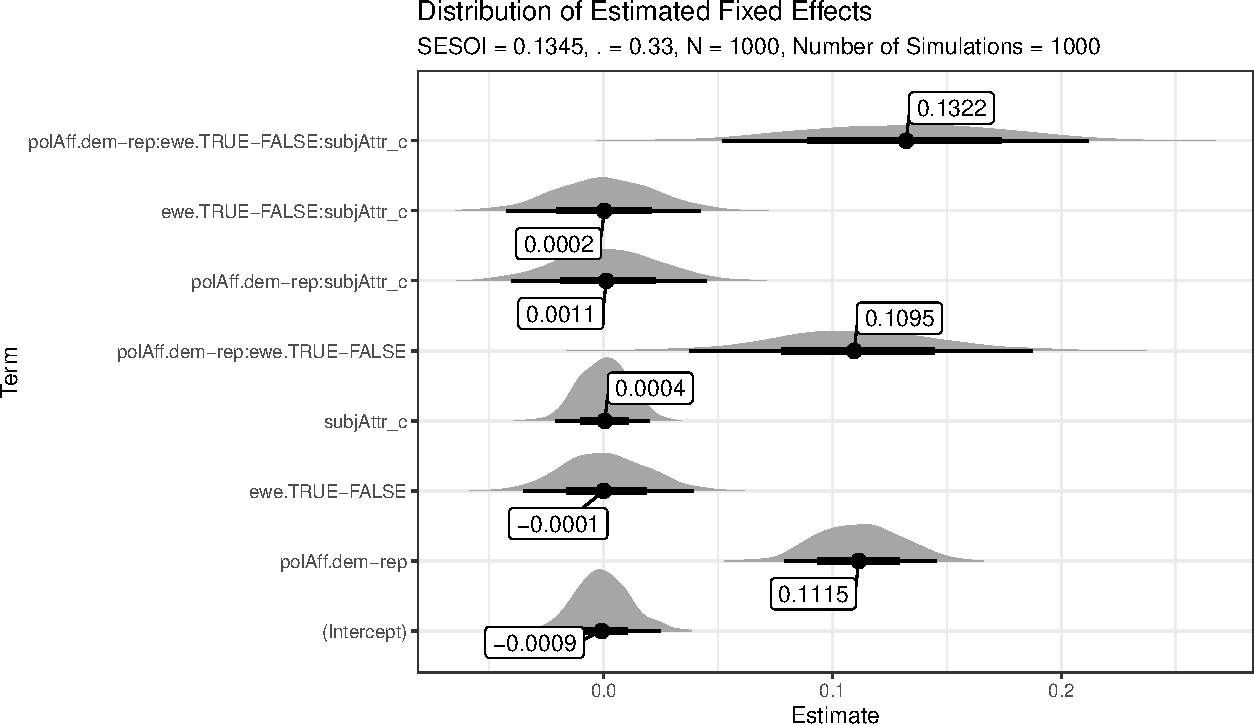
\includegraphics{powerSimulations_files/figure-pdf/fig-checkSims-threeWayInt-1.pdf}

}

\subcaption{\label{fig-checkSims-threeWayInt}}

}

\caption{\label{fig-checkSims-threeWayInt}Distribution of estimated
fixed effects resulting from 1000 simulations for the model
deltaDuration \textasciitilde{} polAff * ewe * subjAttr\_c + (1
\textbar{} subj) + (1 \textbar{} trial). Shaded area represent
densities, annotated points indicate medians, and thick and thin lines
represent 66\% and 95\% quantiles.}

\end{figure}%

Figure~\ref{fig-powC-threeWayInt} shows results of our effect-size
sensitivity analyses. We plot statistical power (y-axis) for different
effect sizes (x-axis), taking into account different assumptions for the
error SD (color) and sample size (panel). Regarding the latter, we
report results not only for the full sample size we aim for (N = 1000),
but also for sample sizes taking into account different participant
exclusion-rates due to exclusion criteria defined in the Registered
Report.

\begin{figure}

\centering{

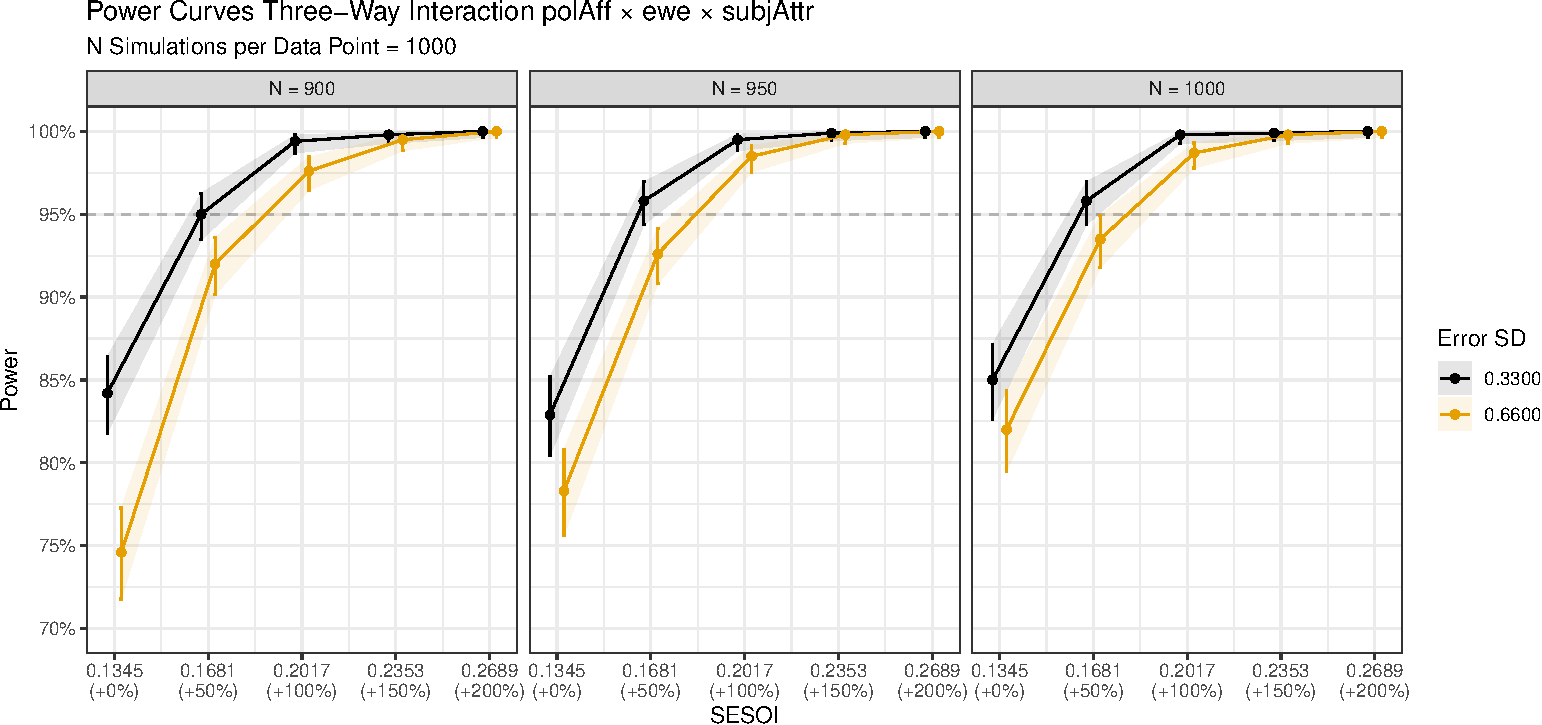
\includegraphics{powerSimulations_files/figure-pdf/fig-powC-threeWayInt-1.pdf}

}

\caption{\label{fig-powC-threeWayInt}Power curves for the three-way
interaction polAff × ewe × subjAttr. Points represent simulated power
surrounded by a 95\%-CI based on 1000 simulations with α = 0.05. Note
that, in contrast to Figure~\ref{fig-powC-mainEffect}, the x-axsis
represents different effect sizes, starting from the defined SESOI,
while the panels represent different sample sizes, taking into account
participant exclusion-rates of 10\% (N = 900), 5\% (N = 950), and 0\% (N
= 1000). Note that estimates are displayed with a slight shift along the
x-axis to reduce overlap.}

\end{figure}%

\begin{Shaded}
\begin{Highlighting}[]
\CommentTok{\# Get power values of interest}
\NormalTok{chosenN }\OtherTok{\textless{}{-}} \DecValTok{950}
\NormalTok{chosenSigma }\OtherTok{\textless{}{-}} \FunctionTok{c}\NormalTok{(}\StringTok{"0.3300"}\NormalTok{, }\StringTok{"0.6600"}\NormalTok{)}
\NormalTok{chosenSESOI }\OtherTok{\textless{}{-}} \FunctionTok{c}\NormalTok{(}\StringTok{"0.1681"}\NormalTok{, }\StringTok{"0.2017"}\NormalTok{)}
\NormalTok{powerValues }\OtherTok{\textless{}{-}}\NormalTok{ resList\_3wayInt.summary }\SpecialCharTok{\%\textgreater{}\%} 
  \FunctionTok{filter}\NormalTok{(sigma\_fact }\SpecialCharTok{\%in\%}\NormalTok{ chosenSigma) }\SpecialCharTok{\%\textgreater{}\%} 
  \FunctionTok{filter}\NormalTok{(sesoi\_fact }\SpecialCharTok{\%in\%}\NormalTok{ chosenSESOI) }\SpecialCharTok{\%\textgreater{}\%} 
  \FunctionTok{filter}\NormalTok{(nSubjects }\SpecialCharTok{\%in\%}\NormalTok{ chosenN)}

\CommentTok{\# Get lower CI for power values for more liberal and more conservative sigma assumptions}
\NormalTok{powerValues\_sigmaLib }\OtherTok{\textless{}{-}}\NormalTok{ powerValues }\SpecialCharTok{\%\textgreater{}\%} 
  \FunctionTok{filter}\NormalTok{(sigma\_fact }\SpecialCharTok{==} \StringTok{"0.3300"}\NormalTok{)}
\NormalTok{powerValues\_sigmaCons }\OtherTok{\textless{}{-}}\NormalTok{ powerValues }\SpecialCharTok{\%\textgreater{}\%} 
  \FunctionTok{filter}\NormalTok{(sigma\_fact }\SpecialCharTok{==} \StringTok{"0.6600"}\NormalTok{)}

\CommentTok{\# Interpolate the effect sizes at which we achieve 95\% power}
\NormalTok{eff\_sigmaLib }\OtherTok{\textless{}{-}} \FunctionTok{approx}\NormalTok{(powerValues\_sigmaLib}\SpecialCharTok{$}\NormalTok{ci.lower, powerValues\_sigmaLib}\SpecialCharTok{$}\NormalTok{sesoi, }\AttributeTok{xout =} \FloatTok{0.95}\NormalTok{)}\SpecialCharTok{$}\NormalTok{y}
\NormalTok{eff\_sigmaCons }\OtherTok{\textless{}{-}} \FunctionTok{approx}\NormalTok{(powerValues\_sigmaCons}\SpecialCharTok{$}\NormalTok{ci.lower, powerValues\_sigmaCons}\SpecialCharTok{$}\NormalTok{sesoi, }\AttributeTok{xout =} \FloatTok{0.95}\NormalTok{)}\SpecialCharTok{$}\NormalTok{y}
\CommentTok{\# Round results for display in text}
\NormalTok{eff\_sigmaLib\_txt\_3way }\OtherTok{\textless{}{-}} \FunctionTok{format}\NormalTok{(}\FunctionTok{round}\NormalTok{(eff\_sigmaLib, }\DecValTok{4}\NormalTok{), }\AttributeTok{nsmall =} \DecValTok{4}\NormalTok{)}
\NormalTok{eff\_sigmaCons\_txt\_3way }\OtherTok{\textless{}{-}} \FunctionTok{format}\NormalTok{(}\FunctionTok{round}\NormalTok{(eff\_sigmaCons, }\DecValTok{4}\NormalTok{), }\AttributeTok{nsmall =} \DecValTok{4}\NormalTok{)}
\end{Highlighting}
\end{Shaded}

To assess the smallest effect size that can be detected with 95\%
statistical power, we inspect the lower bounds of the 95\%-CI power
estimates in Figure~\ref{fig-powC-threeWayInt}. Specifically, we focus
on the power simulation results for N = 950, which takes into account a
participant exclusion rate of 5\%. There, we interpolate between the two
point estimates that lie just below and above the 95\% power line, i.e.,
between the power estimates for effect sizes 0.1681 and 0.2017. Assuming
an error SD of 0.3300, we achieve 95\% statistical power to detect a
three-way interaction effect of at least 0.1728. For a more conservative
error SD of 0.6600, this smallest detectable effect size is only
marginally higher (0.1890).

\section{Conclusion}\label{conclusion}

Using power simulations with mixed-effects models for sample-size
determination and effect-size sensitivity analyses, we show that with a
final sample size of N = 950:

\begin{enumerate}
\def\labelenumi{\arabic{enumi}.}
\item
  We will achieve \textgreater{} 95\% statistical power to detect a main
  effect of political affiliation.
\item
  We will be able to detect a two-way interaction effect of political
  affiliation with extreme weather exposure of at least 0.1619 with ≥
  95\% statistical power.
\item
  We will be able to detect a three-way interaction effect of political
  affiliation with extreme weather exposure and subjective attribution
  of extreme weather events to climate change of at least 0.1890 with ≥
  95\% statistical power.
\end{enumerate}

\begin{tcolorbox}[enhanced jigsaw, arc=.35mm, leftrule=.75mm, opacityback=0, colframe=quarto-callout-note-color-frame, breakable, rightrule=.15mm, toprule=.15mm, left=2mm, colback=white, bottomrule=.15mm]
\begin{minipage}[t]{5.5mm}
\textcolor{quarto-callout-note-color}{\faInfo}
\end{minipage}%
\begin{minipage}[t]{\textwidth - 5.5mm}

\vspace{-3mm}\textbf{Expand for Session Info}\vspace{3mm}

\begin{verbatim}
- Session info ---------------------------------------------------------------
 setting  value
 version  R version 4.4.0 (2024-04-24)
 os       macOS Sonoma 14.4.1
 system   aarch64, darwin20
 ui       X11
 language (EN)
 collate  en_US.UTF-8
 ctype    en_US.UTF-8
 tz       Europe/Zurich
 date     2024-08-16
 pandoc   3.1.11 @ /usr/local/bin/ (via rmarkdown)
 quarto   1.5.45 @ /usr/local/bin/quarto

- Packages -------------------------------------------------------------------
 package     * version  date (UTC) lib source
 binom       * 1.1-1.1  2022-05-02 [1] CRAN (R 4.4.0)
 dplyr       * 1.1.4    2023-11-17 [1] CRAN (R 4.4.0)
 faux        * 1.2.1    2023-04-20 [1] CRAN (R 4.4.0)
 forcats     * 1.0.0    2023-01-29 [1] CRAN (R 4.4.0)
 ggdist      * 3.3.2    2024-03-05 [1] CRAN (R 4.4.0)
 ggeffects   * 1.7.0    2024-06-20 [1] CRAN (R 4.4.0)
 ggplot2     * 3.5.1    2024-04-23 [1] CRAN (R 4.4.0)
 ggpubr      * 0.6.0    2023-02-10 [1] CRAN (R 4.4.0)
 ggrepel     * 0.9.5    2024-01-10 [1] CRAN (R 4.4.0)
 ggthemes    * 5.1.0    2024-02-10 [1] CRAN (R 4.4.0)
 lme4        * 1.1-35.5 2024-07-03 [1] CRAN (R 4.4.0)
 lmerTest    * 3.1-3    2020-10-23 [1] CRAN (R 4.4.0)
 lubridate   * 1.9.3    2023-09-27 [1] CRAN (R 4.4.0)
 Matrix      * 1.7-0    2024-03-22 [1] CRAN (R 4.4.0)
 purrr       * 1.0.2    2023-08-10 [1] CRAN (R 4.4.0)
 readr       * 2.1.5    2024-01-10 [1] CRAN (R 4.4.0)
 sessioninfo * 1.2.2    2021-12-06 [1] CRAN (R 4.4.0)
 stringr     * 1.5.1    2023-11-14 [1] CRAN (R 4.4.0)
 tibble      * 3.2.1    2023-03-20 [1] CRAN (R 4.4.0)
 tictoc      * 1.2.1    2024-03-18 [1] CRAN (R 4.4.0)
 tidyr       * 1.3.1    2024-01-24 [1] CRAN (R 4.4.0)
 tidyverse   * 2.0.0    2023-02-22 [1] CRAN (R 4.4.0)

 [1] /Library/Frameworks/R.framework/Versions/4.4-arm64/Resources/library

------------------------------------------------------------------------------
\end{verbatim}

\end{minipage}%
\end{tcolorbox}

\phantomsection\label{refs}
\begin{CSLReferences}{1}{0}
\bibitem[\citeproctext]{ref-Berger2021}
Berger, Sebastian, and Annika M Wyss. 2021. {``Measuring
Pro-Environmental Behavior Using the Carbon Emission Task.''}
\emph{Journal of Environmental Psychology} 75: 101613.
https://doi.org/\url{https://doi.org/10.1016/j.jenvp.2021.101613}.

\bibitem[\citeproctext]{ref-giner-sorolla2024}
Giner-Sorolla, Roger, Amanda K. Montoya, Alan Reifman, Tom Carpenter,
Neil A. Lewis, Christopher L. Aberson, Dries H. Bostyn, et al. 2024.
{``Power to Detect What? Considerations for Planning and Evaluating
Sample Size.''} \emph{Personality and Social Psychology Review},
February, 10888683241228328.
\url{https://doi.org/10.1177/10888683241228328}.

\bibitem[\citeproctext]{ref-ogunbode2019}
Ogunbode, Charles A., Christina Demski, Stuart B. Capstick, and Robert
G. Sposato. 2019. {``Attribution Matters: Revisiting the Link Between
Extreme Weather Experience and Climate Change Mitigation Responses.''}
\emph{Global Environmental Change} 54 (January): 31--39.
\url{https://doi.org/10.1016/j.gloenvcha.2018.11.005}.

\bibitem[\citeproctext]{ref-reeck2017}
Reeck, Crystal, Daniel Wall, and Eric J. Johnson. 2017. {``Search
Predicts and Changes Patience in Intertemporal Choice.''}
\emph{Proceedings of the National Academy of Sciences} 114 (45):
11890--95. \url{https://doi.org/10.1073/pnas.1707040114}.

\bibitem[\citeproctext]{ref-salthouse2000}
Salthouse, Timothy A. 2000. {``Aging and Measures of Processing
Speed.''} \emph{Biological Psychology} 54 (1): 35--54.
\url{https://doi.org/10.1016/S0301-0511(00)00052-1}.

\bibitem[\citeproctext]{ref-willemsen2019}
Willemsen, Martijn C., and Eric J. Johnson. 2019. {``(Re)visiting the
Decision Factory: Obswerving Cognition with MouselabWEB.''} In, edited
by Michael Schulte-Mecklenbeck, Anton Kuehberger, and Joseph G. Johnson,
2nd ed., 76--95. New York: Routledge.
\url{https://doi.org/10.4324/9781315160559}.

\end{CSLReferences}



\end{document}
